\resetfigpath{Chap3}

%%%{INTRODUCTION to this CHAPTER}%%%
When we are driving, unless no other traffic participants nearby, interactions between drivers happen much more frequent than we realize. Autonomous vehicles, or computer driven vehicles, nowadays are quite adept at driving between lines, make a turn or avoid an obstacles. They are also capable of reacting to humans' behavior, but more often than not, those reactions are not what we expected. This is owing to their incapability of interacting with human. Autonomous vehicles can't communicate with us if they can't understand our gesture or how we usually react to some specific situation. To solve this, we need to develop a model that is able to account for human driver behaviors. The unsignalized crossroads is chosen as the scenario that the model build around for the fact that it is the most communication-requiring traffic scenario, where the other participant's intention to pass or yield is required.

In the following sections, the concepts of time to collision and time for action will be introduced in Section ~\ref{sec:TTCandTFA}. Time to collision and time for action are both key elements for the proposed method, which define the mechanism drivers employed to avoid the potential collision from happening. In Section ~\ref{sec:TFADistribution}, time for action is transformed into a distribution to estimate the chance of braking, and based on this idea, a probabilistic evaluating model is proposed in Section ~\ref{sec:POY}. Finally, to verify and validate the proposed model, experiments at both simulated and real crossroad are conducted in Section ~\ref{sec:ValidatePOY}.


%%%%%%%%%%%%%%%%%%%%%%%%%%%%%%%%%%%%%%%%%%%%%%%%%%%%%%%%%%%%%%%%%%%%%%%%
%%%%%%%%%%               SECTION SECTION SECTION               %%%%%%%%%
%%%%%%%%%%%%%%%%%%%%%%%%%%%%%%%%%%%%%%%%%%%%%%%%%%%%%%%%%%%%%%%%%%%%%%%%

\section{Time to Collision and Time for Action}
\label{sec:TTCandTFA}
When crossing an unsignalized crossroad, the longitudinal speed is decided empirically by human. Drivers observe the oncoming vehicle in a short amount of time and estimate the next possible position, speed and direction it might be, mostly by experience. Then the speed is adjusted accordingly: accelerate to pass the vehicle if drivers \textbf{believe} that arrive at the crossroad before the other participant is possible; or decelerate to yield if a collision is anticipated. Since humans don't perceive the world numerically, researchers have suggested that instead of calculating the distance and the speed directly to define the time to hit an object, more cognitive and abstract methods are used \cite{cog}. In this section, we first introduce the crossroad model. Then, to make driver behavior predictable for computer driven vehicle, researches regarding such mechanism are studied and applied. Finally, a probabilistic model of driving behavior is then developed.

%%%%%%%%------------------------------%%%%%%%%%
%%%%%%%%-----------SUBSECTION---------%%%%%%%%%
%%%%%%%%------------------------------%%%%%%%%%
\subsection{Crossroad Modeling}
\label{sub:crossroad}
A crossroad model where the whole scenario based on is introduced before digging deeper into the driver decision mechanism at the crossroads. Fig.~\ref{fig:model_demo} illustrates a human driver (on the left, heading to the right) and an autonomous vehicle (on the bottom heading upward) crossing a perpendicular crossroad with no signal. Under this circumstance, to reduce the dimensionality of the state space, only on the longitudinal states of concerning vehicles are considered. Also, to prevent confusions, only the interactions between two vehicles are studied at the beginning. In this scenario, \textbf{\emph {the node}} represents the intersection of the extended lines of movement of two traffic agents and would be represented by the symbol like the node in figure Fig.~\ref{fig:model_demo}. 

\begin{figure}[t]
\begin{center}
%\setlength{\unitlength}{0.012500in}
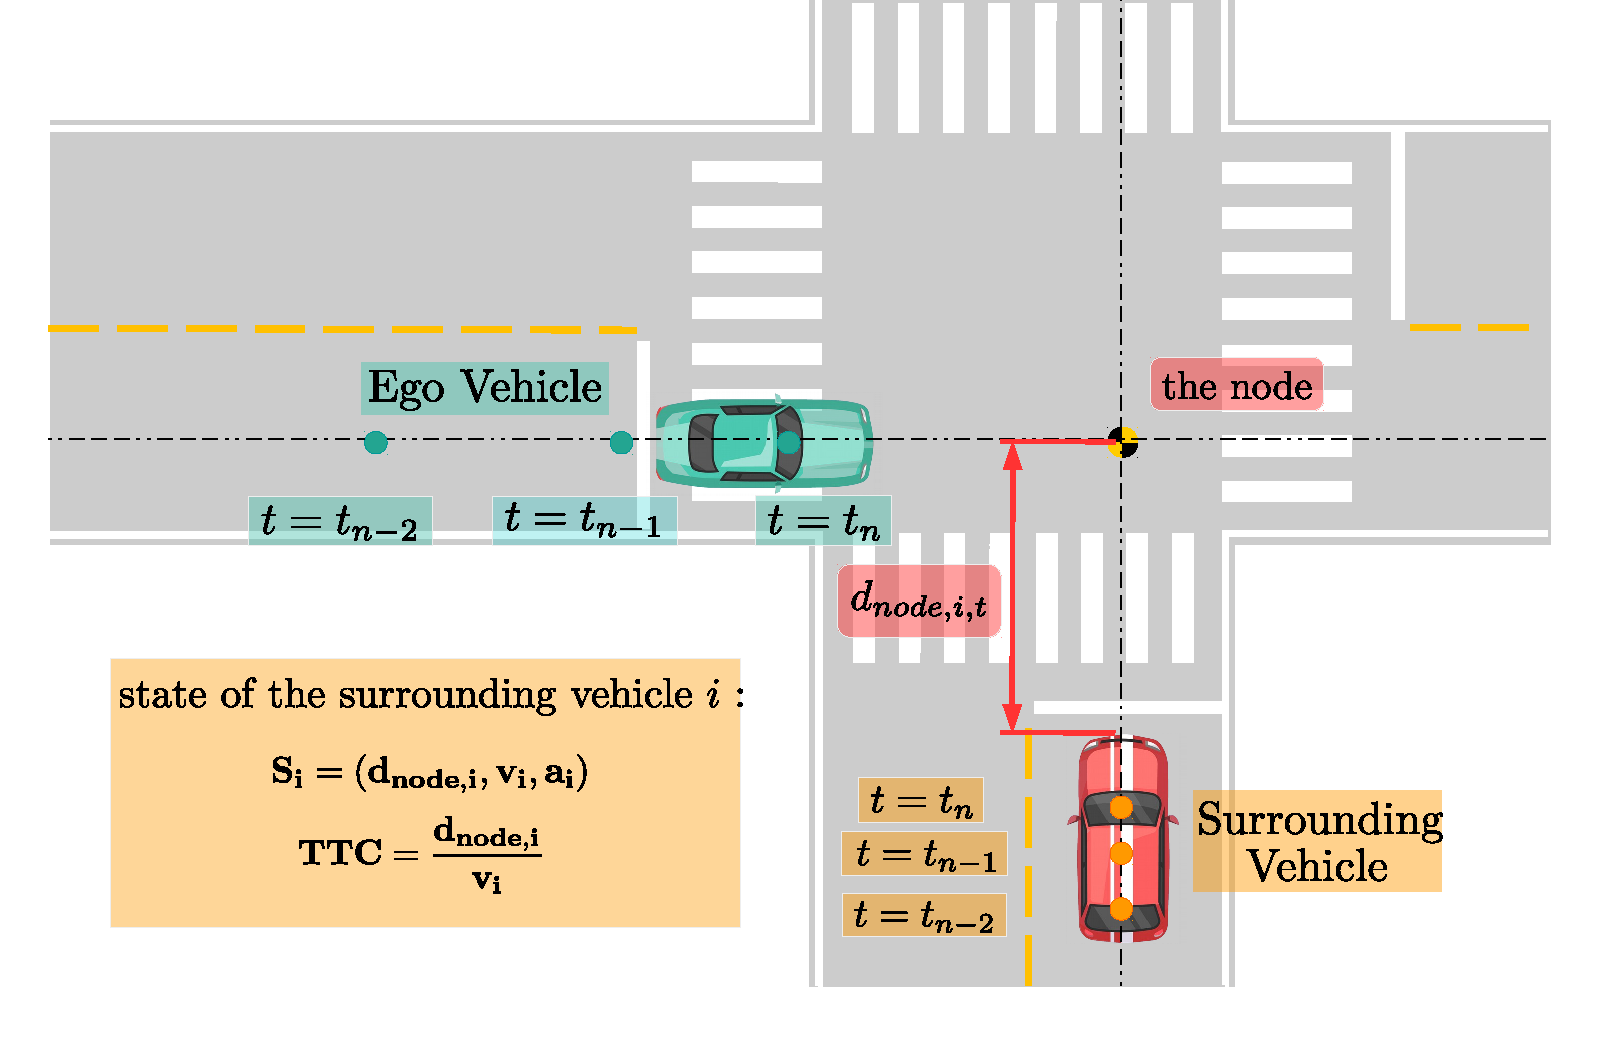
\includegraphics[scale=0.5]{intersection_concept.pdf}
\end{center}
\caption{Demonstration of the proposed scenario and relevant variables.}
\label{fig:model_demo} 
\end{figure}

the node is used as the origin of the coordinate system. The positive $x$ direction is same as the vector of velocity of the first approaching vehicle, and positive $y$ direction as the vector of velocity of the other vehicle. The state of the $i~\text{th}$ vehicle is defined as : 

\begin{equation}
\mathbf{S}_{i,t} = \left( \begin{array}{c} \mathbf{d_{node}}_{i,t} \\ \mathbf{v}_{i,t} \\ \mathbf{a}_{i,t} \end{array} \right), \mbox{ where }  i=\{0, 1, 2, ..., N\} 
\label{eq:state}
\end{equation}

\noindent where $d_{node, i, t}$ is the displacement from the position of the $i~\text{th}$ vehicle to that of the node, $v_{i, t}$ and $a_{i, t}$ are the speed and the acceleration of the $i~\text{th}$ vehicle at time $t$ respectively. Given that $\mathbf{S}_{0}$ is the state of the ego vehicle, $N$ is the number of its surrounding vehicles. Note that they are all one-dimensional. 


As mentioned previously, the main purpose is to find out how human drivers interact with the other moving vehicle as he or she proceeds towards the the node. To focus on this topic, the crossroad model is simplified : only one lane per direction, and one participant driving on each direction. As a consequent, the maneuvers of drivers are reduced to linear motion involving hitting the braking and the gas pedal.  In the following section, the resulting crossroad model is used to determine the mechanism behind the decisions making process of potential collision avoidance.



%%%%%%%%------------------------------%%%%%%%%%
%%%%%%%%-----------SUBSECTION---------%%%%%%%%%
%%%%%%%%------------------------------%%%%%%%%%
\subsection{Time to Collision}
\label{sub:TTC}

How human decide when is the moment to start braking to avoid collision with a stationary obstacle or another moving vehicle has been a popular topic since a couple decades ago \cite{Caird1994}. \ac{TTC}, or time to contact, is a crucial method for human to predict the time it will take to reach the obstacle and take necessary measure to prevent potential collisions from happening. Being an efficient safety measure in traffic safety assessment for decades, TTC was described as “the time required for two vehicles to collide if they continue at their present speed and on the same path.” by Hayward in \cite{Hayward1972}. This concept was usually applied to deal with car following problem, but in this research, it is used to handle vehicle interactions at the crossroad.

The original definition was specified by an optic variable $\tau_{optic}$ ,which is the inverse of the rate of dilation of the object relative to the observer as shown in Eqn.~(\ref{eq:TTC_tau}). 

\begin{equation}
TTC = \frac{\theta_1}{(\theta_2 - \theta_1)/(t_2 - t_1)}
\label{eq:TTC_tau}
\end{equation}

In the Eqn.~(\ref{eq:TTC_tau}), $\theta_1$ and $\theta_2$ are the angular distances of the obstacle's image on the retina at times $t_1$ and $t_2$ separately. Hence the $(\theta_2 - \theta_1)/(t_2 - t_1)$ would be the expansion rate of the obstacle as the observer approaches. However, there are intense disputations over whether $\tau_{optic}$ provides necessary TTC information, since both empirical results and analyses suggest that the hypothesis is false, as described in \cite{tau}. 

There also exist another potential way to describe TTC involving the information of the speed and the distance to the target object, as described in Eqn.~(\ref{eq:TTC_dv}).

\begin{equation}
TTC = \frac{\text{distance to obstacle}}{\text{speed}}
\label{eq:TTC_dv}
\end{equation}

Also known as cognitive or computational strategy, this method takes account of the distance from the obstacle (the target object) and the speed assessed by the driver. To verify this idea, Cavallo et al. \cite{TTC} conduct a series of experiments in real driving condition. Volunteers of different ages, genders and experience levels in driving were asked to estimate the time it would take to collide with the obstacle. The results suggested that both speed and distance information are taken into account in TTC estimation. 

Since the TTC definition in Eqn.~(\ref{eq:TTC_dv}) is more applicable and also verified in the literature, in this research the speed and the distance to the intersection are used as variables to describe the human driver behaviors in proposed model. 


%%%%%%%%------------------------------%%%%%%%%%
%%%%%%%%-----------SUBSECTION---------%%%%%%%%%
%%%%%%%%------------------------------%%%%%%%%%
\subsection{Time for Action}
\label{sub:TFA}

TTC provides a way to imitate the method used by human drivers when facing a potential collision event. However, the goal is to predict the other participant's decision, that is, to pass or to yield, and the mechanism of this decision is still unclear. To explain the decision making process, we will introduce the new term "\ac{TFA}".

To fully understand the role of TFA in braking decision, first the definition of TTC is used to explain how the braking decision is made : under a given speed, the driver decides to brake to avoid collisions when a certain distance is left between the car and the obstacle. As shown in Fig.~\ref{fig:TTC_history}, a car is approaching from the left while a red obstacle is on its path. At point $P_A$, the car is cruising with constant speed $V_0$. The driver should have already observed the obstacle but he or she feels no pressure to brake at this point. As the car keeps moving forward, the driver realizes that if he or she does not brake here, the vehicle might collide with the red obstacle. After the brake being applied at $P_B$, the car begins to slow down and finally comes to a stop with the speed equals to $0$ at point $P_C$. 

In this scenario, TTC decreases as the distance to the obstacle is getting shorter. Finally at point $P_B$, the driver decides to brake to keep a safe margin from the vehicle to the obstacle when the car is fully stopped. The distance from point $P_B$ to the obstacle is the "distance left before action", which is the minimum distance required to stop in front of the obstacle and keep the safe margin in between. Now we divide this distance by the speed at point $P_B$, we get this TTC where the driver take the action to avoid the collision. We call this TTC "Time for Action (TFA)". 

The time-history of TTC and the dependent variables depicted in Fig.~\ref{fig:example_TTC_TFA} are put together and presented in Fig.~\ref{fig:TTC_history}. The figure used here is similar to the time-history of braking presented in the work of Winsum et al. \cite{time_history}. The motion of the vehicle cruising from point $P_A$ to $P_B$ in Fig.~\ref{fig:example_TTC_TFA} results in the TTC drops from $t=0$ to $t=t_0$ in Fig.~\ref{fig:TTC_history}. This is due to the decrease of the distance to the obstacle while the speed of the vehicle is constant. Then the driver brakes at point $P_B$ in Fig.~\ref{fig:example_TTC_TFA} as the driver brakes at time $t_0$ in Fig.~\ref{fig:TTC_history}. 

\begin{figure}[htbp!]
\begin{center}
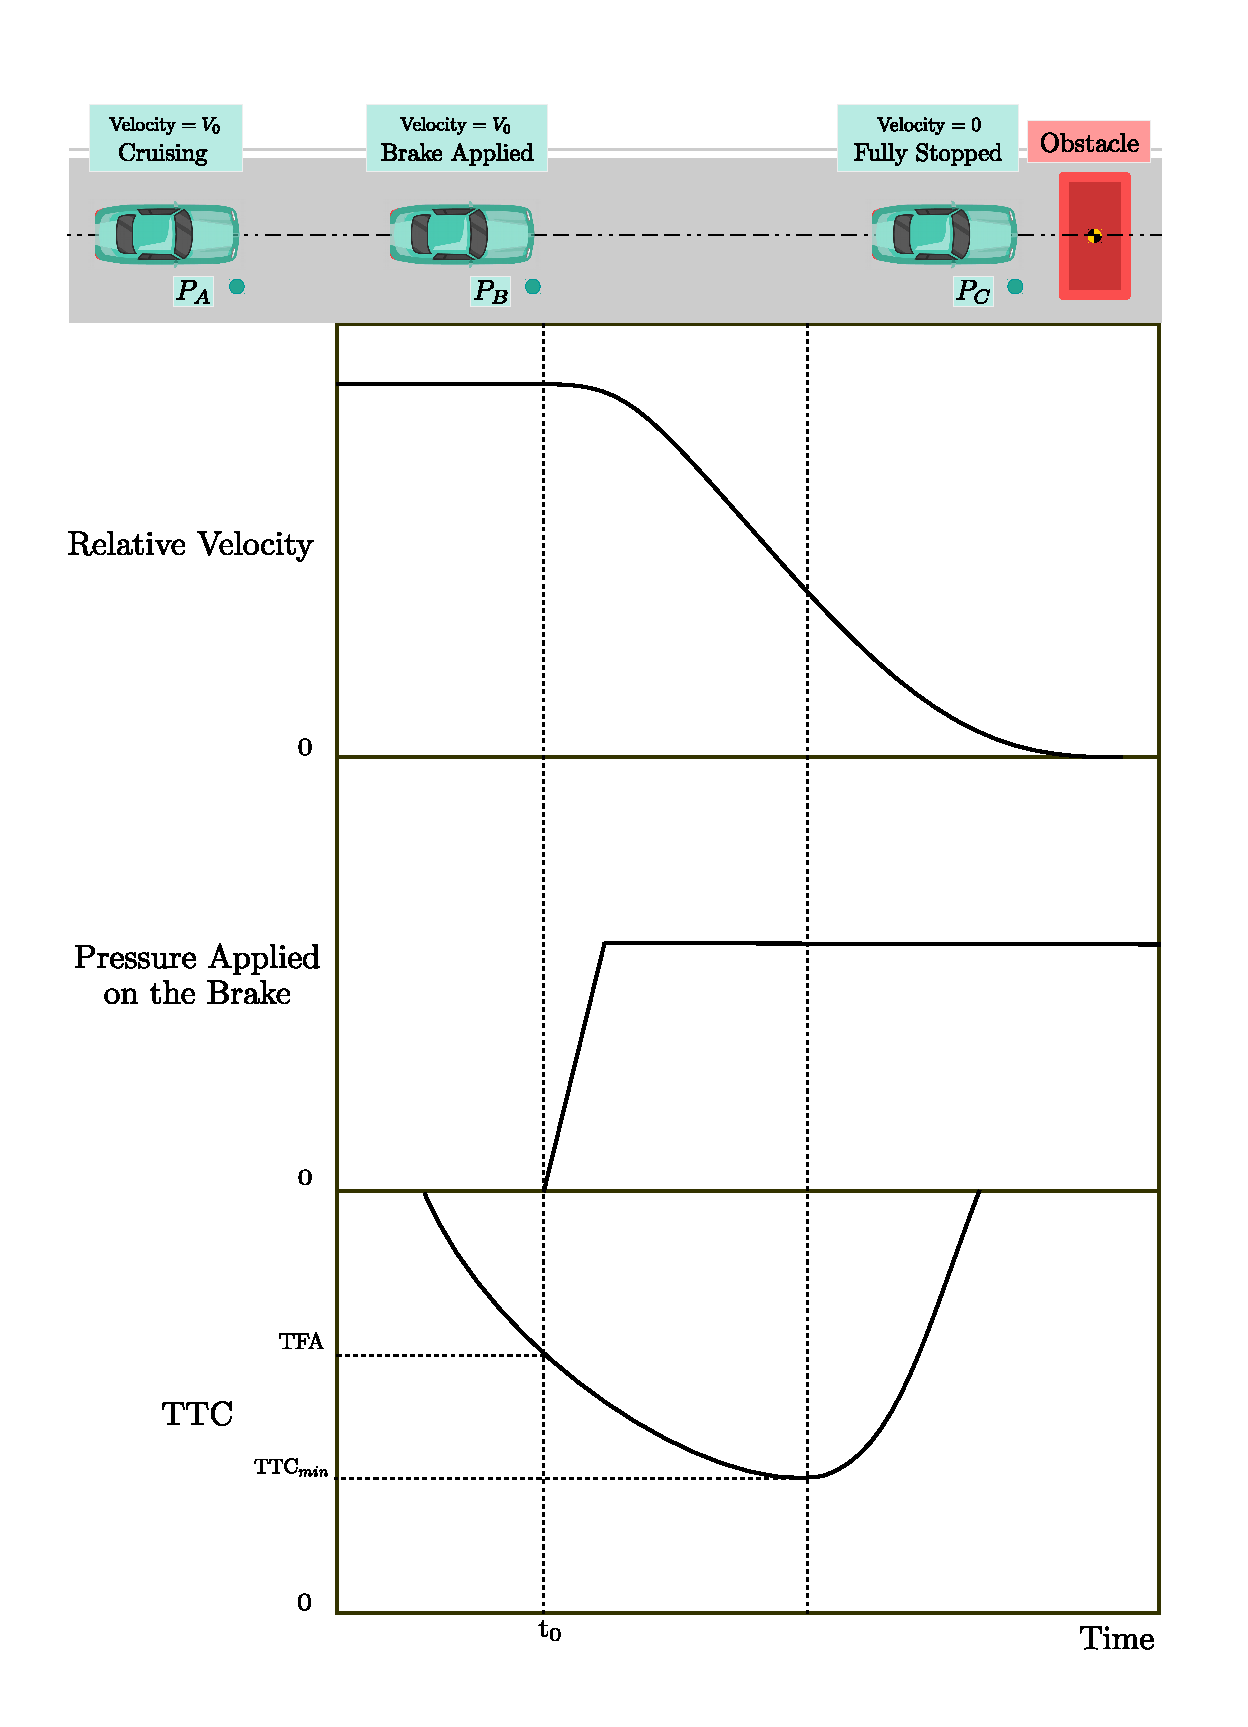
\includegraphics[scale=0.63]{TTC_change_when_braking.pdf}
\end{center}
\caption{History of time to collision when brake is applied.}
\label{fig:TTC_history} 
\end{figure}

The TTC value at this instance should equal to TFA of the driver under this speed by definition since this is the TTC he or she believes that a collision would happen if the brake is applied any later. During the braking, TTC drops to its lowest point labeled as $TTC_{min}$ and then rises. The rise is due to the the speed decreasing rate (i.e. acceleration) being higher than the rate of the distance decrease (i.e. the speed). Note the TFA is the minimum TTC that drivers start to hit the brake to avoid collision, not the minimum TTC during the whole process (which is the $TTC_{min}$ in Fig.~\ref{fig:TTC_history}).

From the above paragraph we know that not solely speed or distance is utilized in the decision of braking, it is the TTC which formulated using the combined information of both variables that driver perceived take parts in the mechanism. In the crossroad scenario, when a vehicle is about to arrive at the crossroad at the same time as the host vehicle, the host vehicle driver subconsciously imagines the future position of the oncoming vehicle, which turns out to be a real obstacle exist at the point of intersection due to the fact that the only location of the potential collision is at the intersection of two perpendicular paths (as shown in Fig.~\ref{fig:imagine_obstacle}). Despite there is not really an obstacle lying right in the middle of the crossroad, we tend to prevent the worst case from happening by estimating the next possible position of the oncoming vehicle with the tangential path. We can adjust our speed accordingly to avoid the potential collision.  

\begin{figure}[htbp!]
\begin{center}
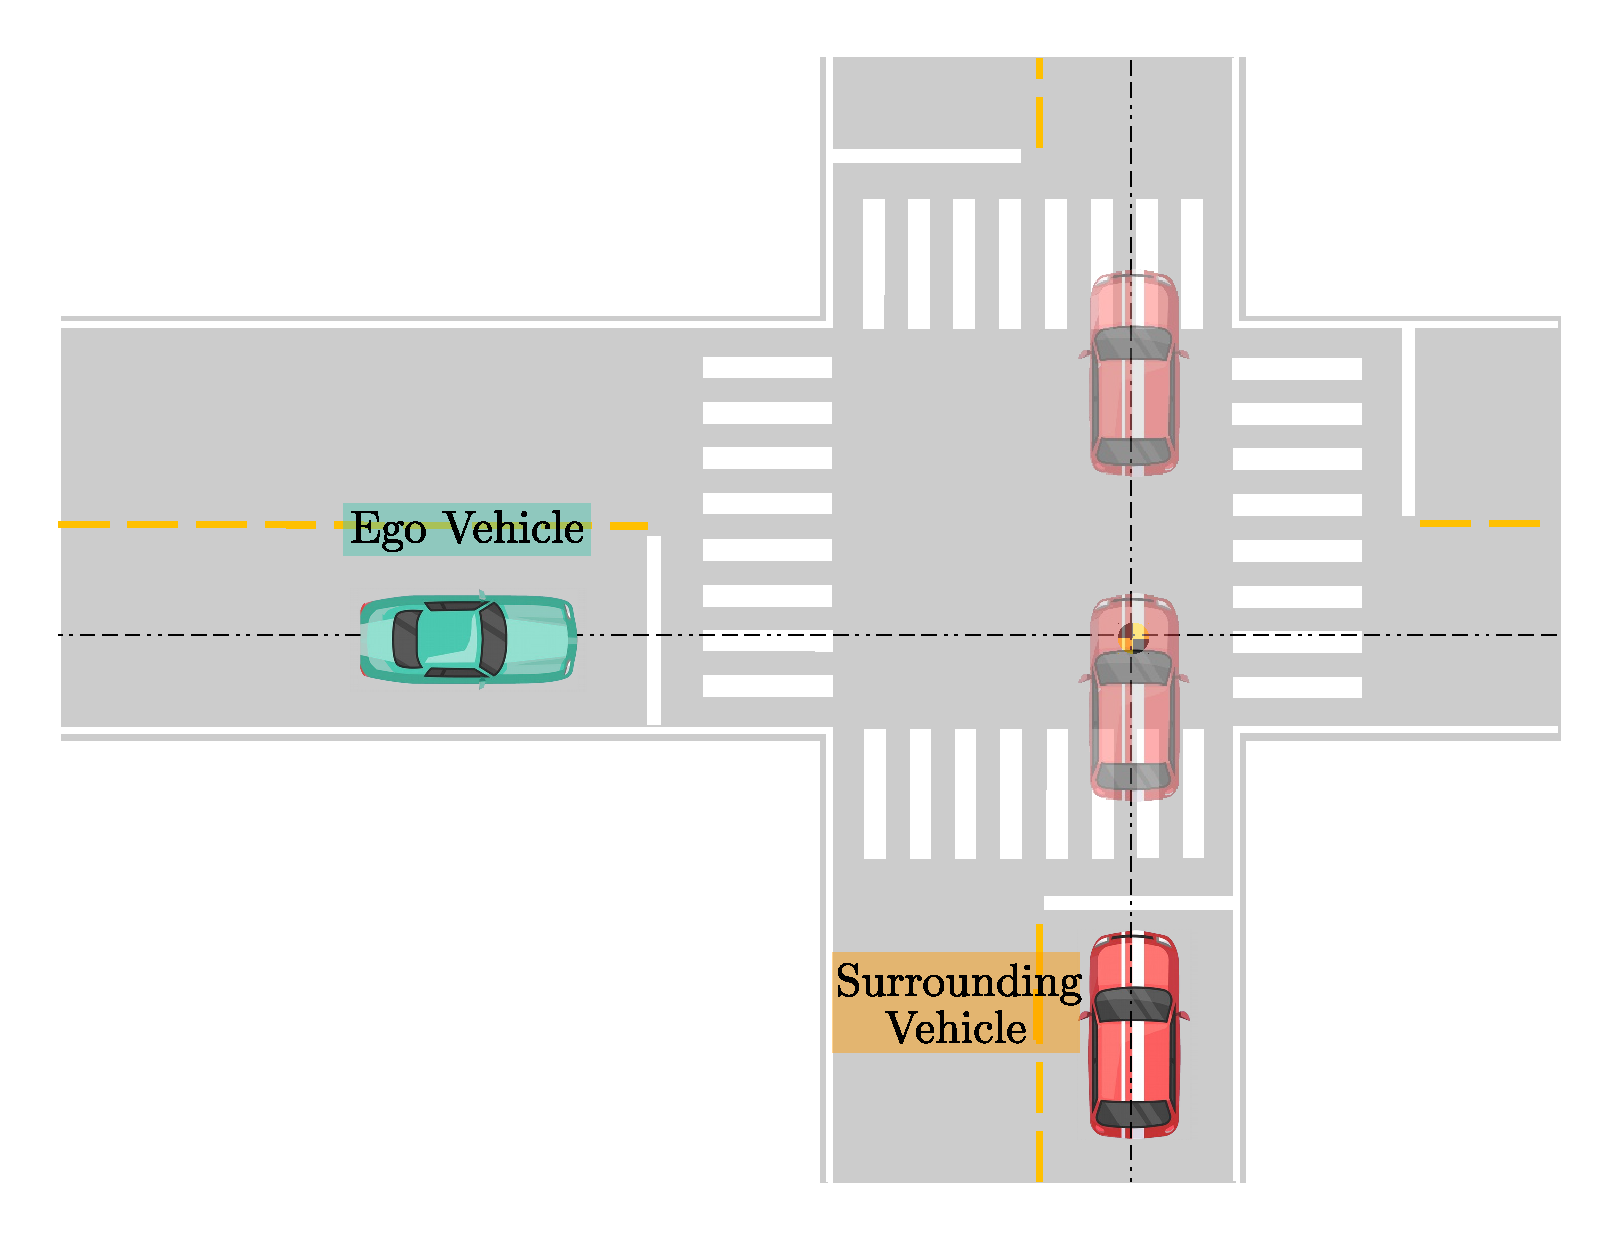
\includegraphics[scale=0.43]{intersection_imagining_obstacle.pdf}
\end{center}
\caption{The host driver estimate the possible position of the oncoming vehicle depending on its current states. To avoid the potential collision, the host driver adjust the time to brake as if the oncoming vehicle is at the intersection.}
\label{fig:imagine_obstacle} 
\end{figure}

Now let us bring TTC and TFA into our crossroads scenarios. Since TTC here can be estimated using the distance to the intersection and the current speed of the vehicle while the TFA is the same as in the situation which a real obstacle exists at the intersection, combining Eqn.~(\ref{eq:state}) and Eqn.~(\ref{eq:TTC_dv}) we have : 

\begin{equation}
\mathbf{TTC} = \frac{\mathbf{d_{node,i}}}{\mathbf{v_{i}}}
\label{eq:TTC_crossroad}
\end{equation}

In this case, at the moment the host driver sees the oncoming vehicle and thinks that it might collide with him, he or she would put the foot on the brake while the TTC is dropping. Then, the brake would finally be applied at the instance that the TTC he cognized is equivalent to his TFA, so the potential collision at the node (the intersect of two routes) would be avoided. Note that the $\mathbf{d_{node,i}}$ here represents the \textit{displacement} instead of the distance for the purpose of distinguishing two opposite sides of the node, in other words, the displacement is adopted to separate the states before and after passing the node. So, the direction the host vehicle faces would always be the positive on the coordinate system. Throughout this research, the use of displacement and distance are interchangeable since the situations that we are interested in happen before the node (i.e. the displacement is always positive).



It is clear until now that the particular moment of decision making at the crossroad is accessible if both TTC and TFA are able to be determined. The TTC can be calculated without effort by dividing the displacement to the node by the speed of the subjective vehicle. However, there is little discussion about the concept of TFA in the literature. Also, even if the access to the very TFA of the driver is possible, which in fact only an approximated value could be acquired, it is still not guaranteed that the driver will hit the brake at that exact moment since the randomness of the human perception and the resulting errors while generating the actions. This issue will be addressed thoroughly in the following section.

In the previous sections, the literature concerning psychology and cognitive science is investigated to determine the deciding component (i.e. TTC and TFA) in human drivers' braking event. Then, both variables are applied in the crossroad scenarios as illustrated in ~\ref{sub:crossroad}. In the next section, an assumption that is capable of explaining the stochastic character of TFA will be established. Then a probabilistic model of drivers behavior based on the concepts of TTC and TFA will be proposed to handle the stochastic decision process of human at the crossroad. 


%%%%%%%%%%%%%%%%%%%%%%%%%%%%%%%%%%%%%%%%%%%%%%%%%%%%%%%%%%%%%%%%%%%%%%%%
%%%%%%%%%%               SECTION SECTION SECTION               %%%%%%%%%
%%%%%%%%%%%%%%%%%%%%%%%%%%%%%%%%%%%%%%%%%%%%%%%%%%%%%%%%%%%%%%%%%%%%%%%%
\section{ The TFA Distribution}
\label{sec:TFADistribution}
In this section, the concept of TFA distribution is described. TFA distribution is the fundamental idea to this research an it is what the proposed model is built upon. Following this concept, we are able to obtain the probability density function of TFA from which the probability of the vehicle yielding could be determined using the proposed model.

%%%%%%%%------------------------------%%%%%%%%%
%%%%%%%%-----------SUBSECTION---------%%%%%%%%%
%%%%%%%%------------------------------%%%%%%%%%
\subsection{TFA Distribution}
\label{sub:TFA Distribution}

From the above paragraph we know that the definition of TFA is the minimum TTC (or the minimum distance left before braking at the current speed) that drivers start to hit the brake to avoid potential collision.This decision making process will differ from person to person since each of us has our own risk threshold to decide the braking timing. For example, a young driver with a high performance sports car might have a relatively low TFA because of his personality and the great braking performance of the car which allows the driver to go closer before braking. On the contrary, an older driver driving an aged passenger sedan might have a higher TFA since the driver is more cautious and the car requires longer distance to stop.

\begin{figure}[htbp!]
\begin{center}
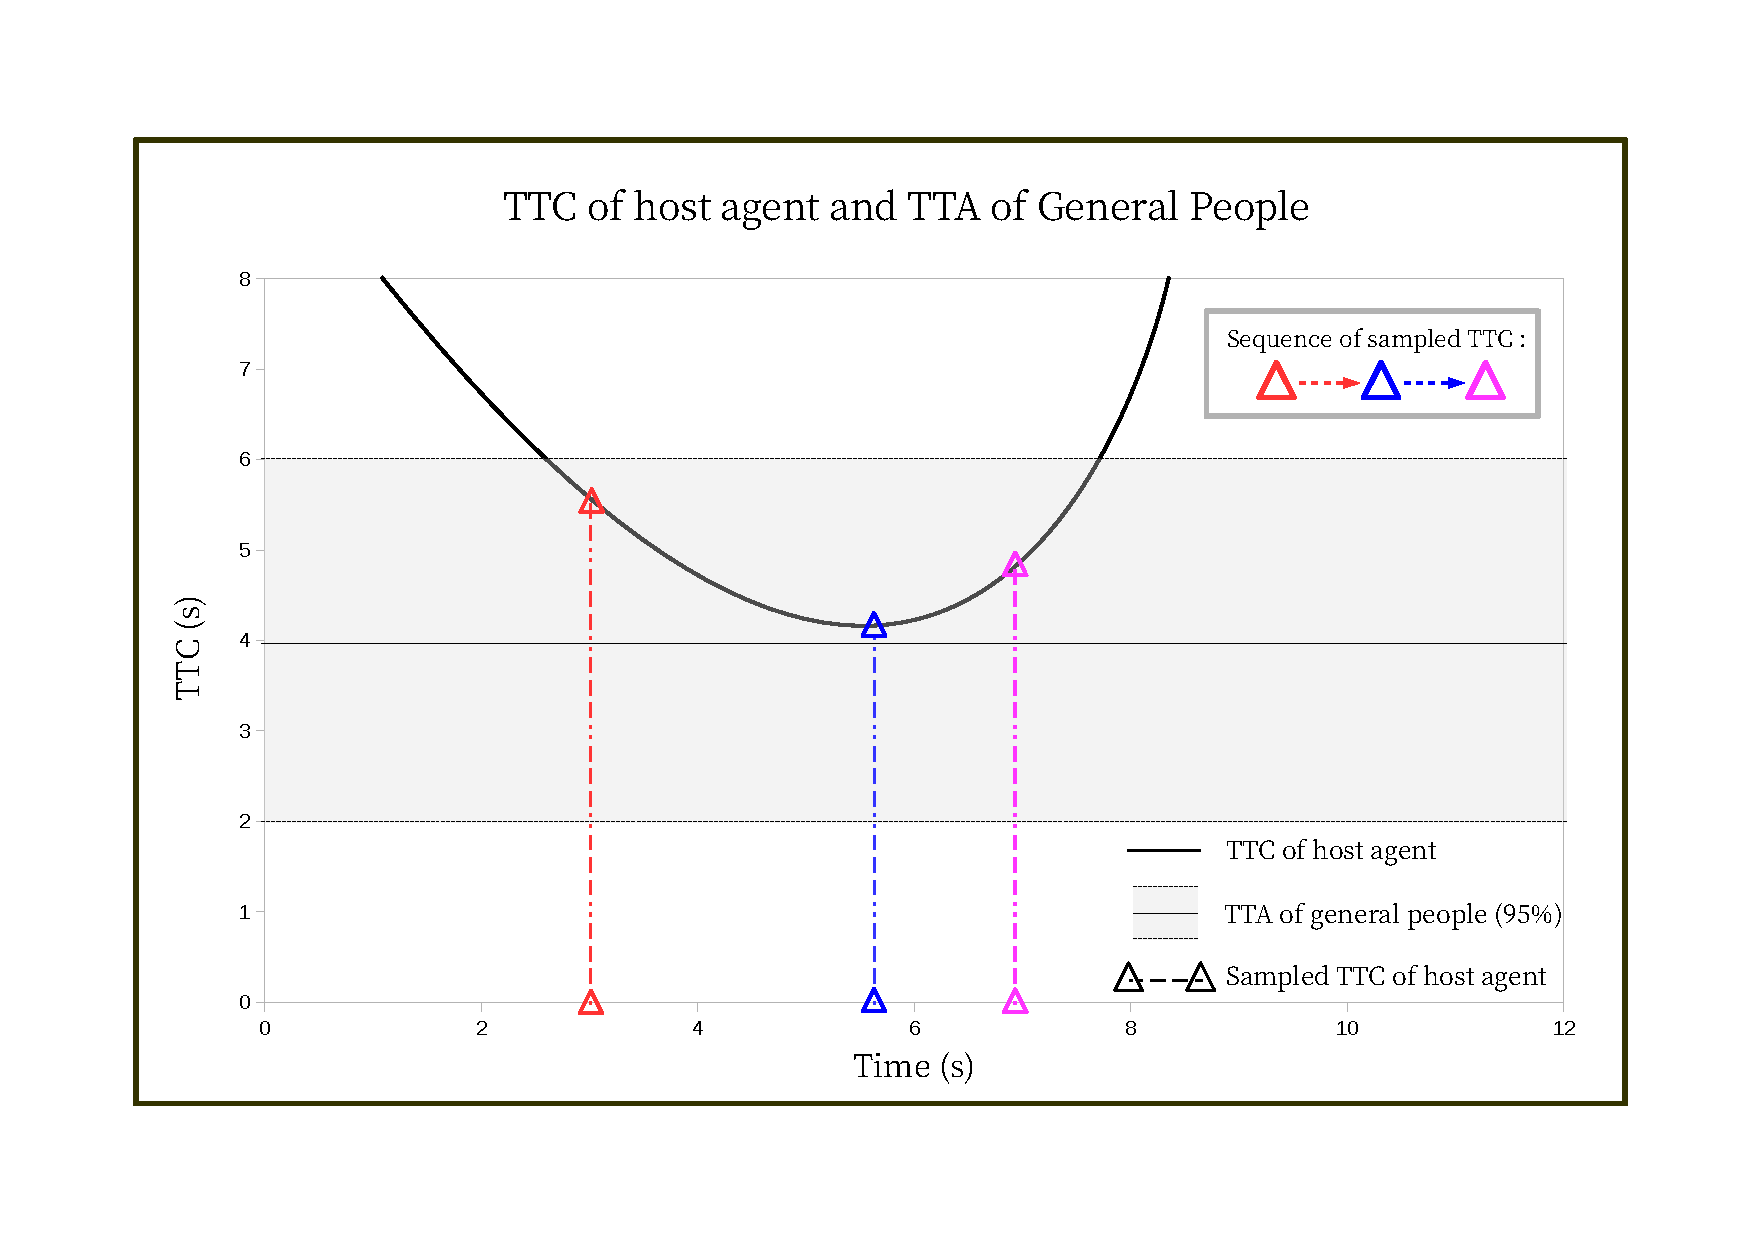
\includegraphics[scale=0.5]{TTC_probability.pdf}
\end{center}
\caption{Example of TFA of general people and TTC of the host agent.}
\label{fig:TTC_TFA} 
\end{figure}

This idea is illustrated in Fig.~\ref{fig:TTC_TFA}. In Fig.~\ref{fig:TTC_TFA}, grey area is drew to illustrate the distribution of TFA of general people (95\% of people's TFAs are within the area) while solid line is indicating the TTC of the host agent changing with time, which is similar to that in Fig.~\ref{fig:TTC_history}. The distribution of TFA can be explained as "within this range of TTC, 95\% of drivers will initiate the action (hit the brake) if potential collisions exist". So in the crossroad scenario where two vehicles are about to reach the intersection at the same time, when the TTC of one of the drivers is getting lower, we can infer that his or her chance of braking to yield is getting higher because more and more people in the distribution start braking as it goes. 

In fact, not only is the TFA of different people a distribution, but the TFA of a person under different personal or environmental conditions also is a distribution. However, there is rarely any literature conducted such experiments, so the assumption that TFA distributions are normally distributed is made. The reason behind this assumption is that even if the distributions of the perception and the motion during the action process (which is braking in this content) are not normally distributed, the combined outcome of these independent random variables would still approximate a Normal distribution, given large enough samples. 

In spite of the fact that this idea is supported by the Central Limit Theorem, experiments are conducted to support the assumption. Both Relative Judgement tasks or Prediction-motion tasks are often employed in the literature to estimate the ability of the participant to derive TTC information . In Relative Judgement tasks, subjects are required to indicate the first arriving moving target from two approaching ones. In the Prediction-motion tasks, on the other hand, subjects are asked to predict the time of the moving object arrive at a specified position after the moving object disappeared from the view. In these tasks, subjects are making decisions while watching a pre-recorded film. 

However, it is hardly possible for subjects to identify the TFA without knowing how the vehicle will response while the brake is applied. Consequently, to make it more similar to the driving scenario in real world, a simulated crossroad environment is constructed. Detailed discussion regarding the simulated crossroad as well as how the experiments are conducted will be delivered in the following sections where model validation is conducted. For now, the focus is put on the distribution of TFA.

In the experiments, three volunteers are asked to drive toward a static vehicle with constant speed and apply the brake when they believe that the collision will happen if it is applied any later. TFAs in this scenario would be the displacement from the host vehicle to the static vehicle divided by speed of the host vehicle at the moment which brake is applied. Results are shown in Fig.~\ref{fig:TFA_distr_1}, Fig.~\ref{fig:TFA_distr_2} and Fig.~\ref{fig:TFA_distr_3}. Noted that the distribution of TFA might varies under different speed, but only the parameters of the distribution are changed, not the type of the distribution. The focus now is on weather the TFA could be modeled as a normal distribution ,the property of TFA distributions under different speed will be discussed later. 

\begin{figure}[htbp!]
\begin{center}
\makebox[0pt]{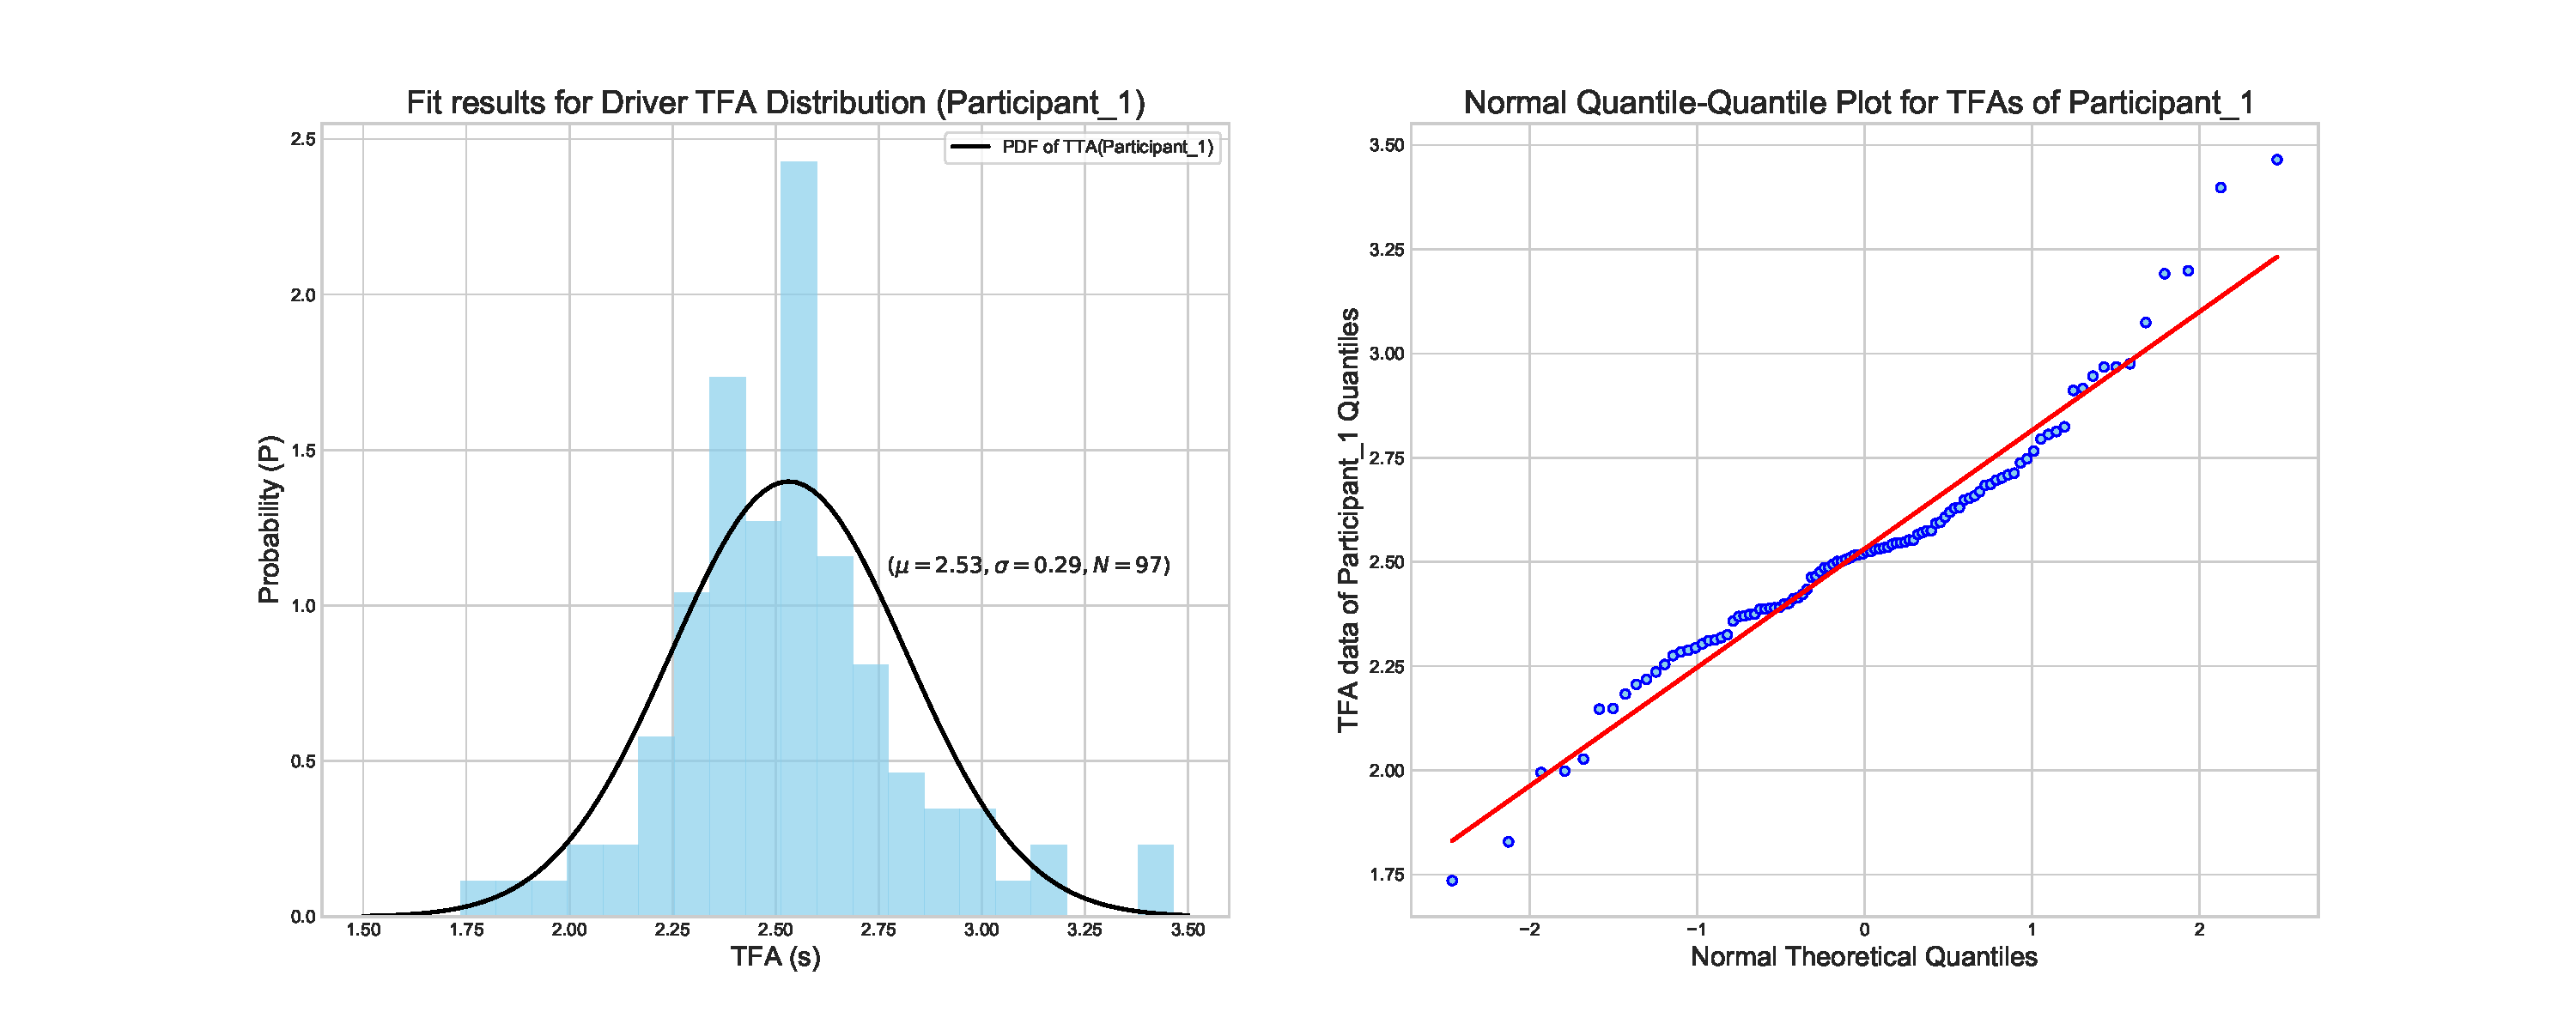
\includegraphics[width=0.8\paperwidth]{Participant_1_0_fitting.pdf}}
\end{center}
\caption{TFA results of participant 1 displayed in histogram. The solid curve is the TFA distribution of participant 1 approximated by Normal distribution ($\mu = 2.35, \sigma = 0.29, N = 97$). Speed of the vehicle while braking was set to 5 m/s. }
\label{fig:TFA_distr_1} 
\end{figure}

\begin{figure}[htbp!]
\begin{center}
\makebox[0pt]{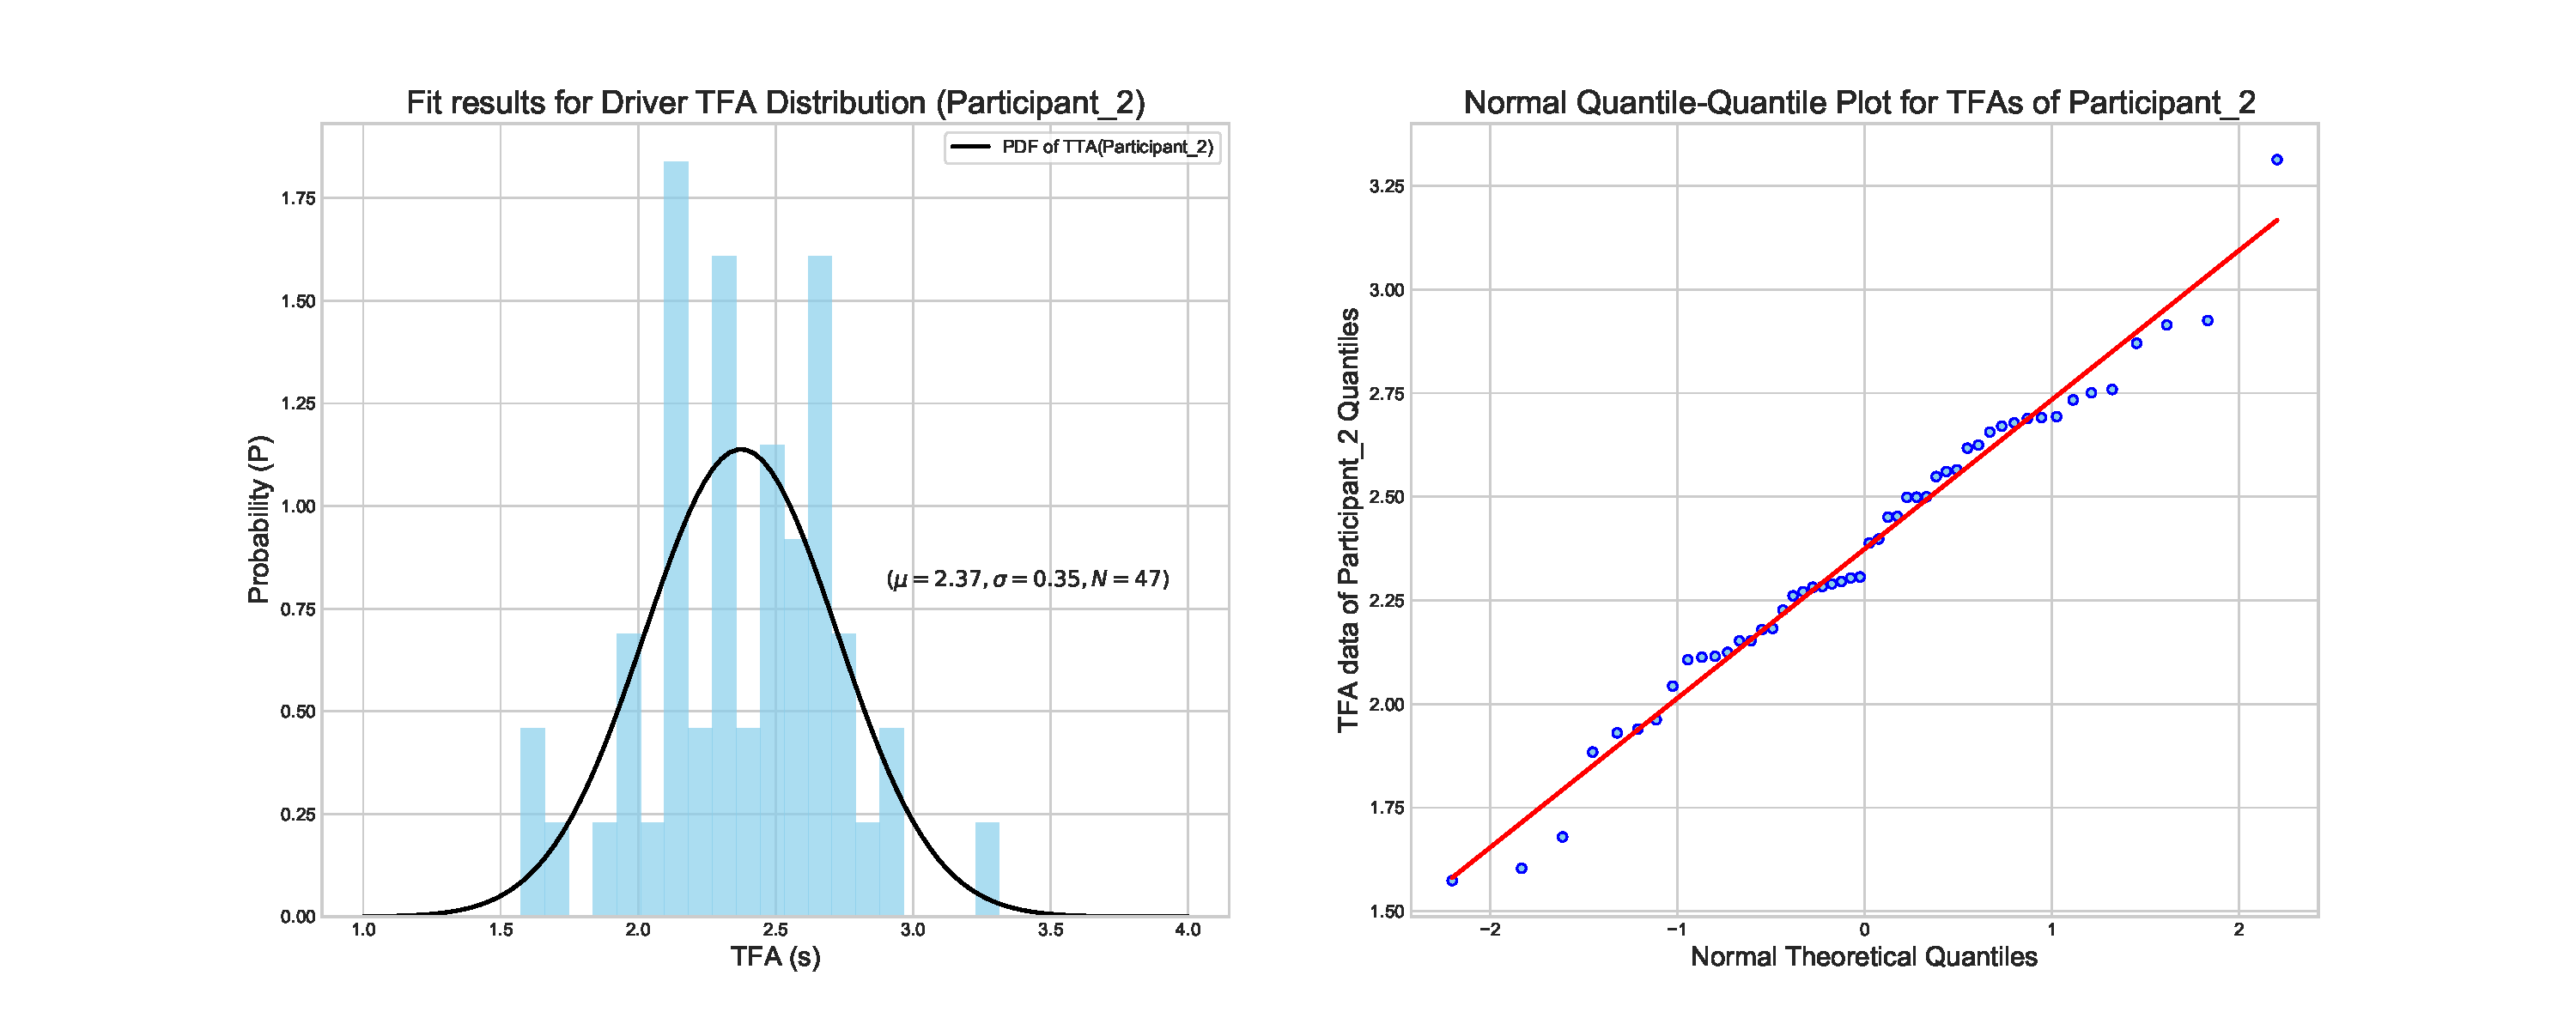
\includegraphics[width=0.8\paperwidth]{Participant_2_0_fitting.pdf}}
\end{center}
\caption{TFA results of participant 2 displayed in histogram. The solid curve is the TFA distribution of participant 2 approximated by Normal distribution ($\mu = 2.37, \sigma = 0.35, N = 47$). Speed of the vehicle while braking was set to 5 m/s.}
\label{fig:TFA_distr_2} 
\end{figure}

\begin{figure}[htbp!]
\begin{center}
\makebox[0pt]{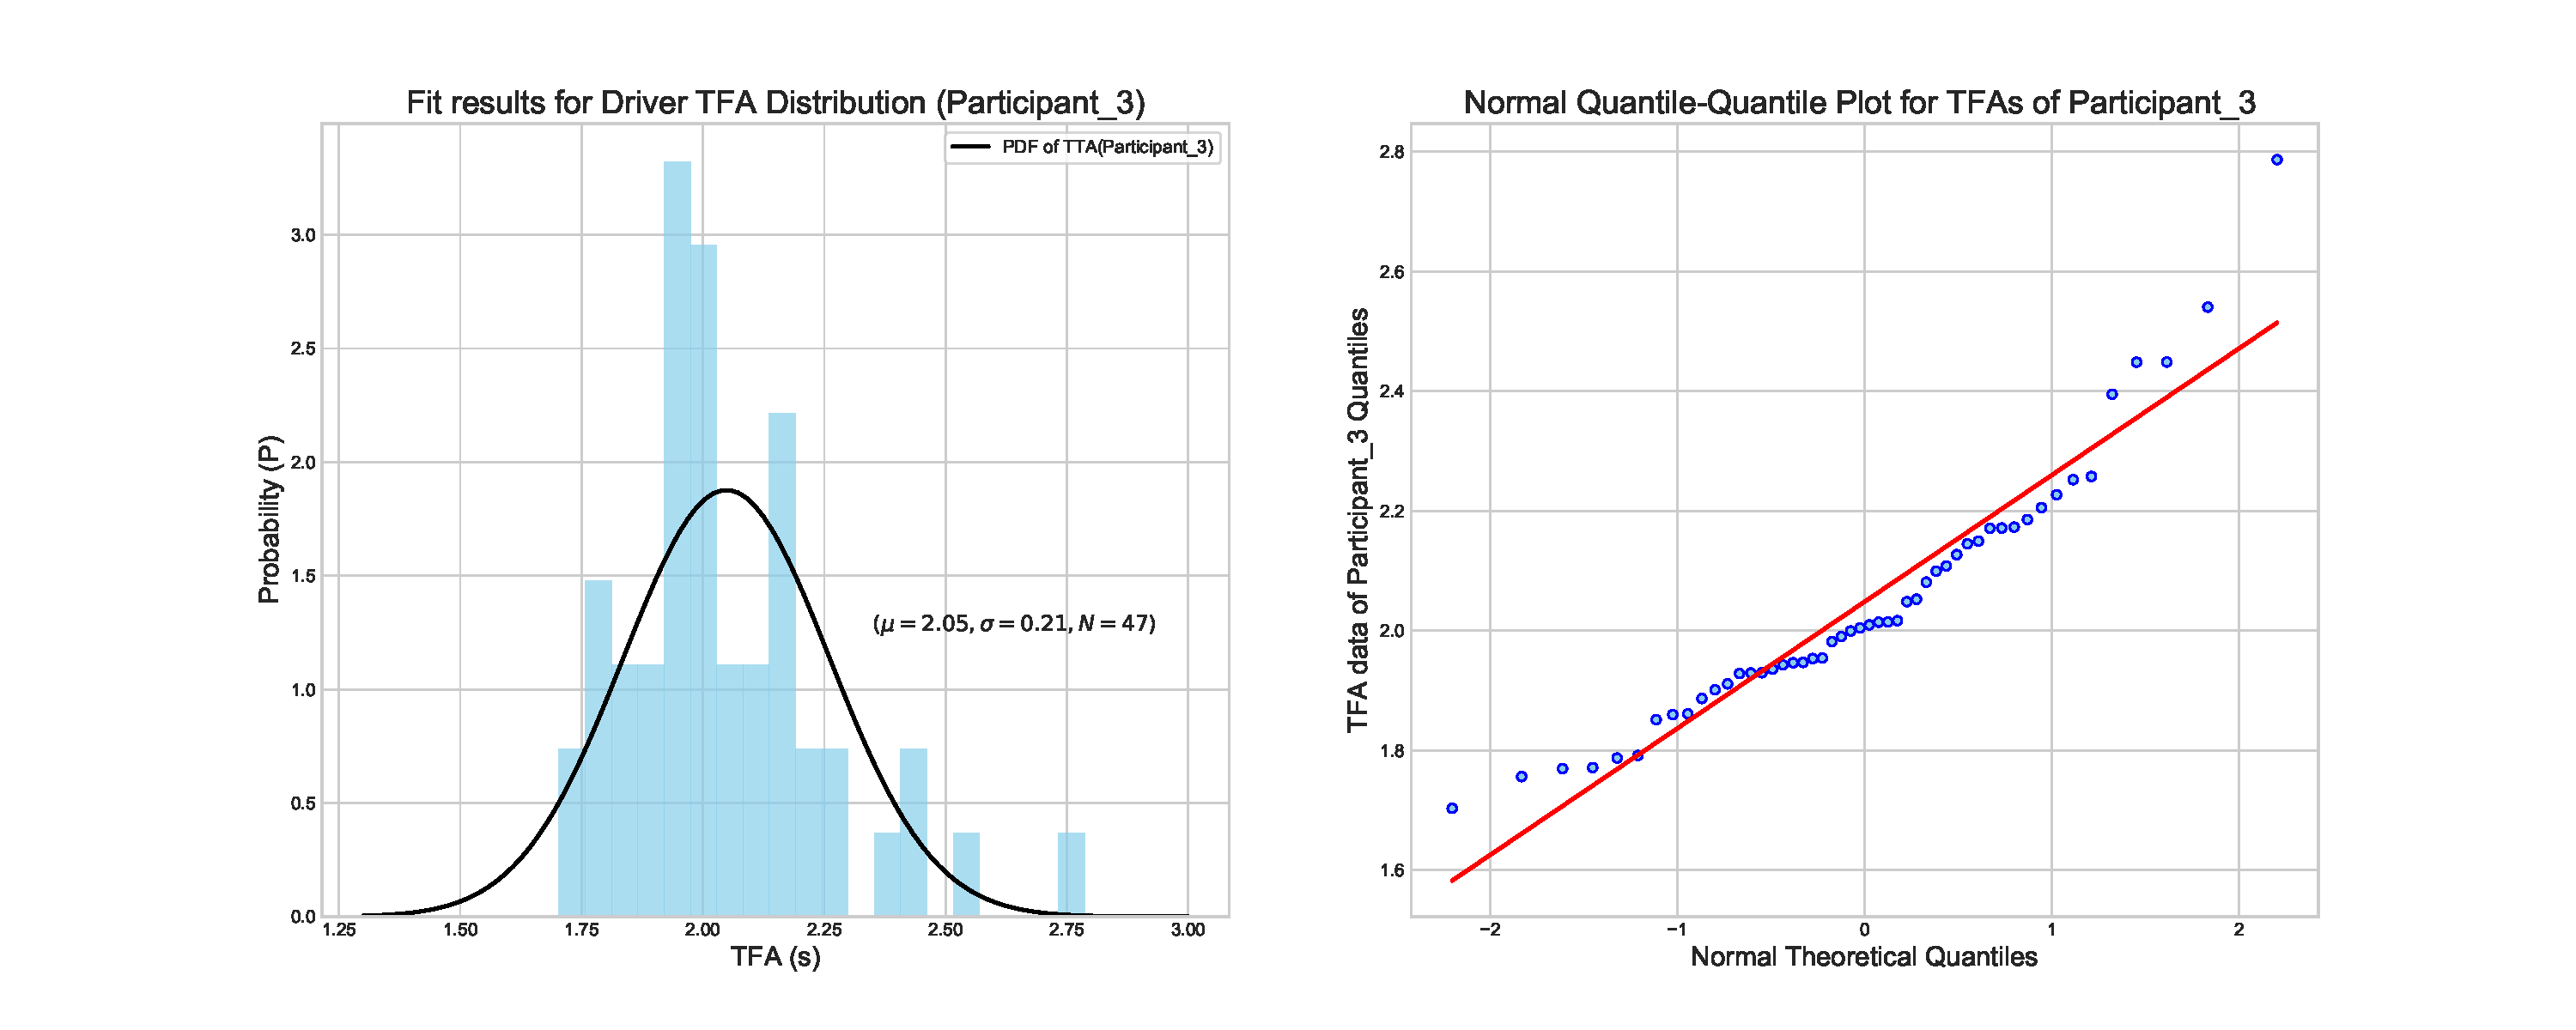
\includegraphics[width=0.8\paperwidth]{Participant_3_0_fitting.pdf}}
\end{center}
\caption{TFA results of participant 3 displayed in histogram. The solid curve is the TFA distribution of participant 3 approximated by Normal distribution ($\mu = 2.05, \sigma = 0.21, N = 47$). Speed of the vehicle while braking was set to 5 m/s.}
\label{fig:TFA_distr_3} 
\end{figure}

In Fig.~\ref{fig:TFA_distr_1}, Fig.~\ref{fig:TFA_distr_2} and Fig.~\ref{fig:TFA_distr_3}, sub-figures on the left are experimental TFA results plotted in histograms while sub-figures on the right are \ac{Q-Q Plots} using the same sets of TFA data. Q-Q plot is a graphical tool that can be used to examine the plausibility of the examined data coming from a theoretical distribution which is the Normal distribution in our case. One should note that Q-Q plots are merely a visual checking method that can give us an idea of how close the distribution of sampling data is comparing to theoretical one. Red solid lines in each figures are standard lines representing the theoretical results if the subject distribution is also a Normal distribution, in other words, closer the points to the red line higher chance the subject data is normally distributed.  

What we can learn from the figures is that TFA distribution of a single driver can be approximated by the Normal distribution if given large enough number of samples. To examine whether the TFA of general people is also normally distributed, all TFA data of participants are combined together in Fig.~\ref{fig:TFA_distr_combined}. Although the number of volunteers is not large enough, we can still learn from Fig.~\ref{fig:TFA_distr_combined} that combined distribution of drivers' TFA can also be approximated by Normal distribution. This result is actually unsurprising providing that all three individual TFA distributions are normally distributed.

\begin{figure}[htbp!]
\begin{center}
\makebox[0pt]{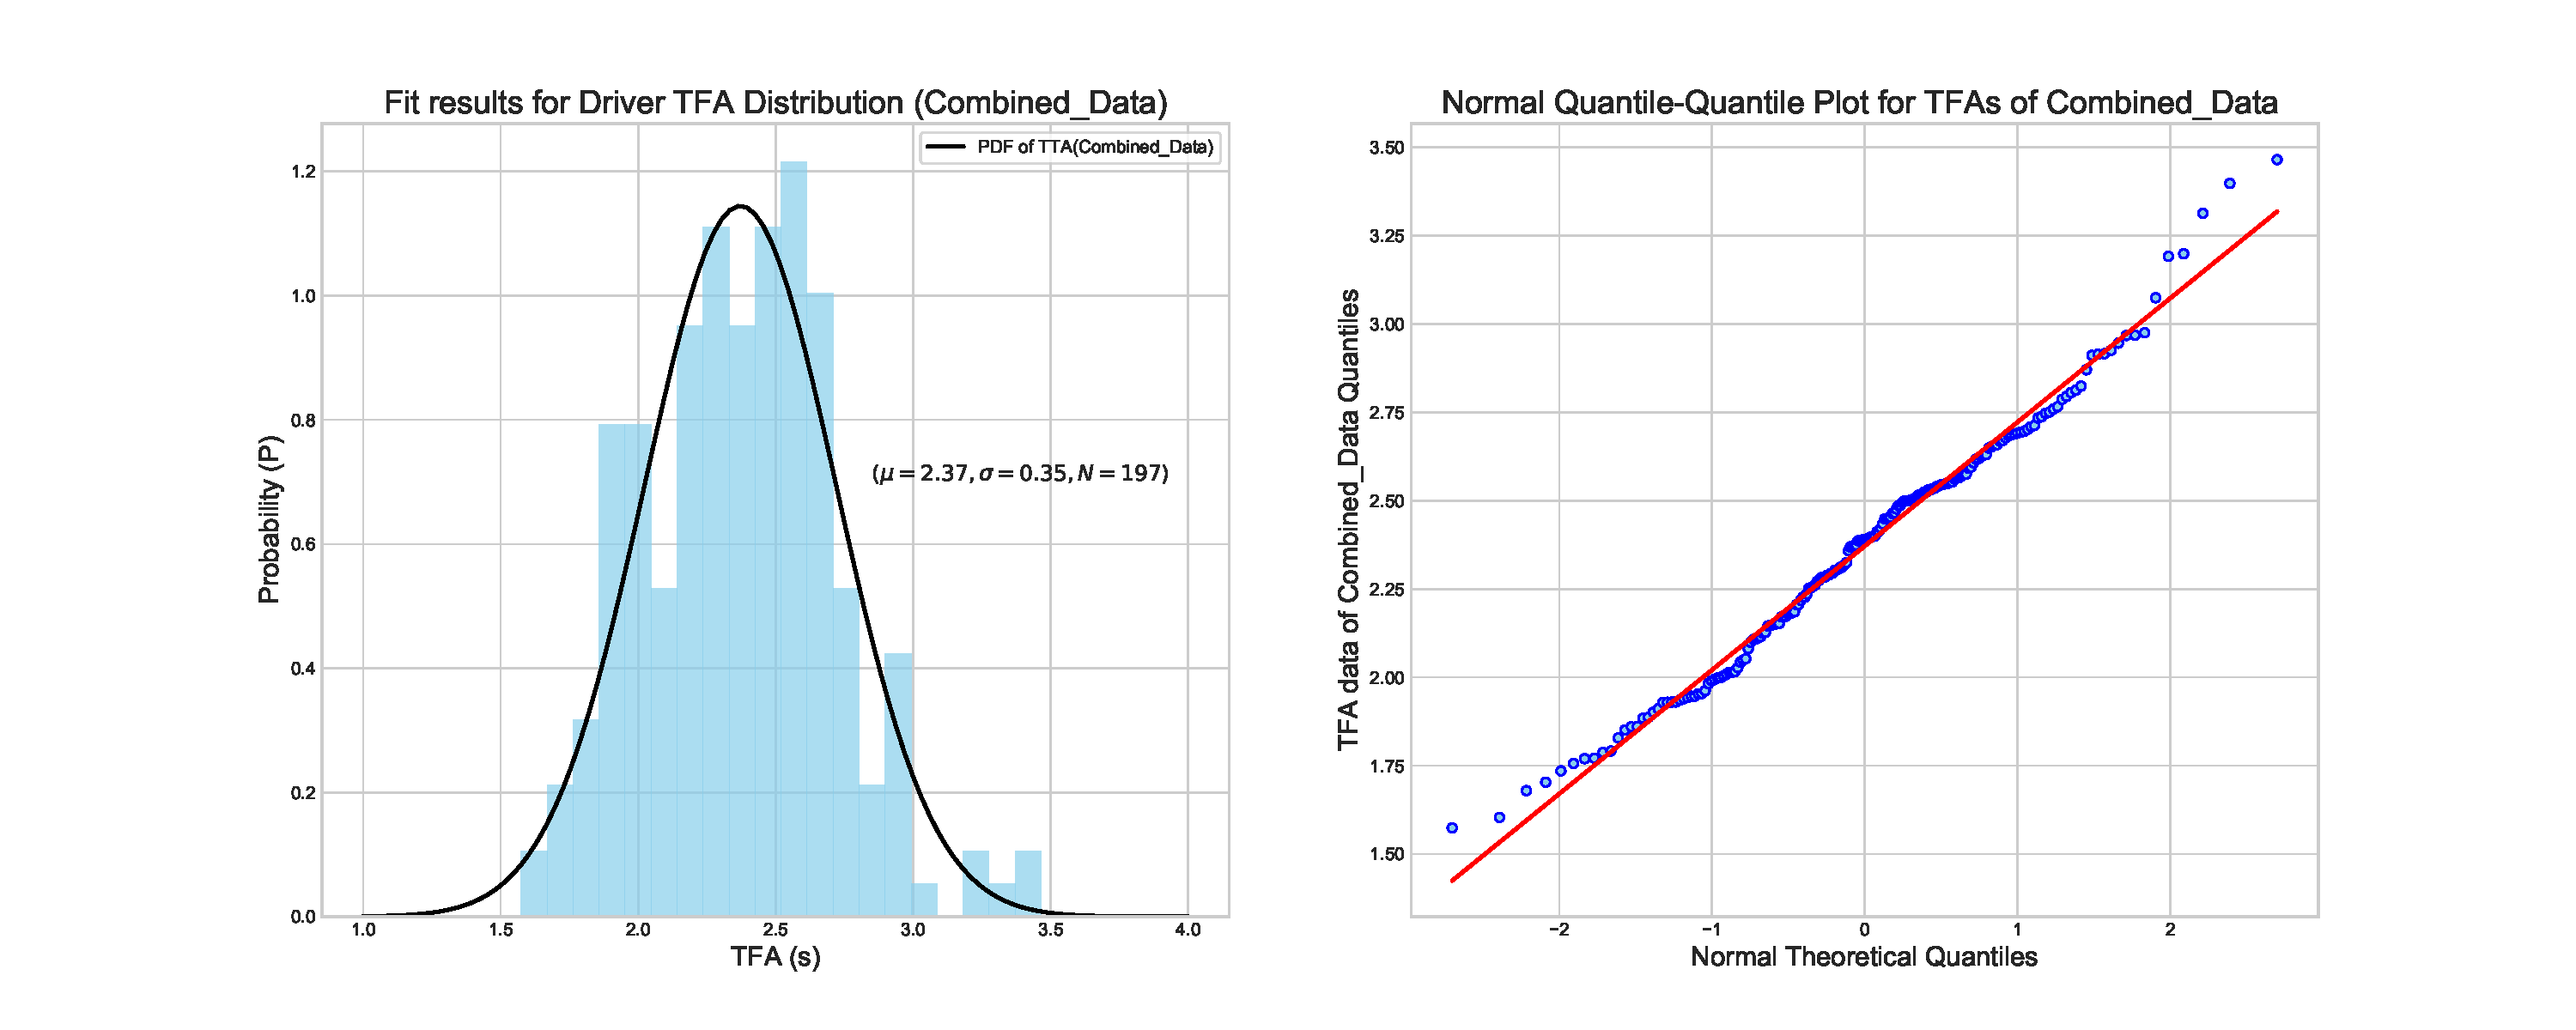
\includegraphics[width=0.75\paperwidth]{Combined_Data_0_fitting.pdf}}
\end{center}
\caption{TFA results of all participants are displayed in histogram. The solid curve is the TFA distribution of combined data of participants approximated by Normal distribution ($\mu = 2.37, \sigma = 0.35, N = 197$). Speed of the vehicle while braking was set to 5 m/s.}
\label{fig:TFA_distr_combined} 
\end{figure}

Knowing the TFA distribution for both individual and general people can be approximated by Normal distribution, the probability of a driver braking could be inferred effortlessly using the probability density function of the Normal distribution.

 
%%%%%%%%------------------------------%%%%%%%%%
%%%%%%%%-----------SUBSECTION---------%%%%%%%%%
%%%%%%%%------------------------------%%%%%%%%%
\subsection{TFA Probability Density Function}
\label{sub:TFA PDF}

From the previous section, the distribution of TFA is identified. In order to describe the human decision making process in a probabilistic way, the probability density function (PDF) of the TFA distribution is used. PDF is a function that defines the continuous random variables. A point on the PDF represents the \textit{likelihood} that the value of the random variable equals the sample value. Hence, an area under the curve of PDF would stand for the \textit{probability} of the random variable falling within that range. 

We can turn the grey area in Fig.~\ref{fig:TTC_TFA} into a PDF as in Fig.~\ref{fig:TTC_distribution}. In this case, when a certain value of TTC within the PDF of TFA of general people is reached, the area under the PDF and right to this value represents the probability of the brake being applied. To make it clearer, let us assume the TTC of a vehicle driving towards a crossroad now is 3. At this instance, the probability for the driver to brake would then be the area under the PDF and right to the value 3, which is 50\% since 3 is also the mean value of the TFA distribution in Fig.~\ref{fig:TTC_distribution}. Drivers with TFA greater than 3 would have braked before the TTC reached 3 because the TTC drops as the host vehicle is driven toward the crossroad and the displacement to the node is decreasing according to Eqn.~\ref{eq:TTC_crossroad}. The concept behind using the area under the PDF and right to the current TTC as the probability to brake combines elements introduced in the previous sections, including using TTC as to indicate the time for braking (i.e. TFA) and approximating the TFA distribution with Normal distribution.

What should be noted here is that since whether the driver brakes or not, the displacement to the node during that time is always decreasing. According to Eqn.~\ref{eq:TTC_crossroad}, if the constant car speed is maintained, the value of TTC will fall down as the vehicle is driven toward the node. On the other hand, if the brake is applied, the TTC rises parabolically as shown in Fig.~\ref{fig:TTC_history}. Hence, before the brake is applied, the TTC used to calculate the probability is the TTC at the moment. The TTC used to calculate the probability after the brake is applied should then be the lowest TTC that occurs on the TTC curve of the host agent since the intention to brake during the braking process remains the same as the beginning of the action. We will use Fig.~\ref{fig:TTC_TFA_indicator} and ~\ref{fig:TTC_distribution} to further explain this idea. 

In Fig.~\ref{fig:TTC_TFA_indicator}, the dashed lines indicated by colored shapes (including squares, triangles and circles) on both sides represent the sampled moments during the braking process. Red squares indicating the TTC at 3 seconds on the time line, blue triangles at around 5.5 seconds and magenta circles at around 7 seconds. The corresponding moments are also labeled on the TFA distribution in Fig.~\ref{fig:TTC_distribution}. At 3 seconds (red squared connected with dashed line, using red line in short) the TTC of the host agent is around 4.2 seconds. We can then estimate from the PDF in Fig.~\ref{fig:TTC_distribution} that the probability of the vehicle stopping is 0.0013, which is the area right side of the red line. This result is reasonable since the TTC at this moment is still far from the TFA average which is 3. Similarly, when the time is at 5.6 seconds (blue line) the TTC at the time is around 3.1, so the probability of the vehicle stops rise to 0.401. As it comes to the time at 7 seconds (magenta line) the TTC becomes larger due to the brake, but as mentioned before, the rising of TTC indicates the agent is slowing down, which does not lower the probability to brake. So the probability of the host agent braking is still calculated using the lowest TTC value on the TTC curve which is 3.1, so the probability to brake is still 0.401.

\begin{figure}[htbp!]
\begin{center}
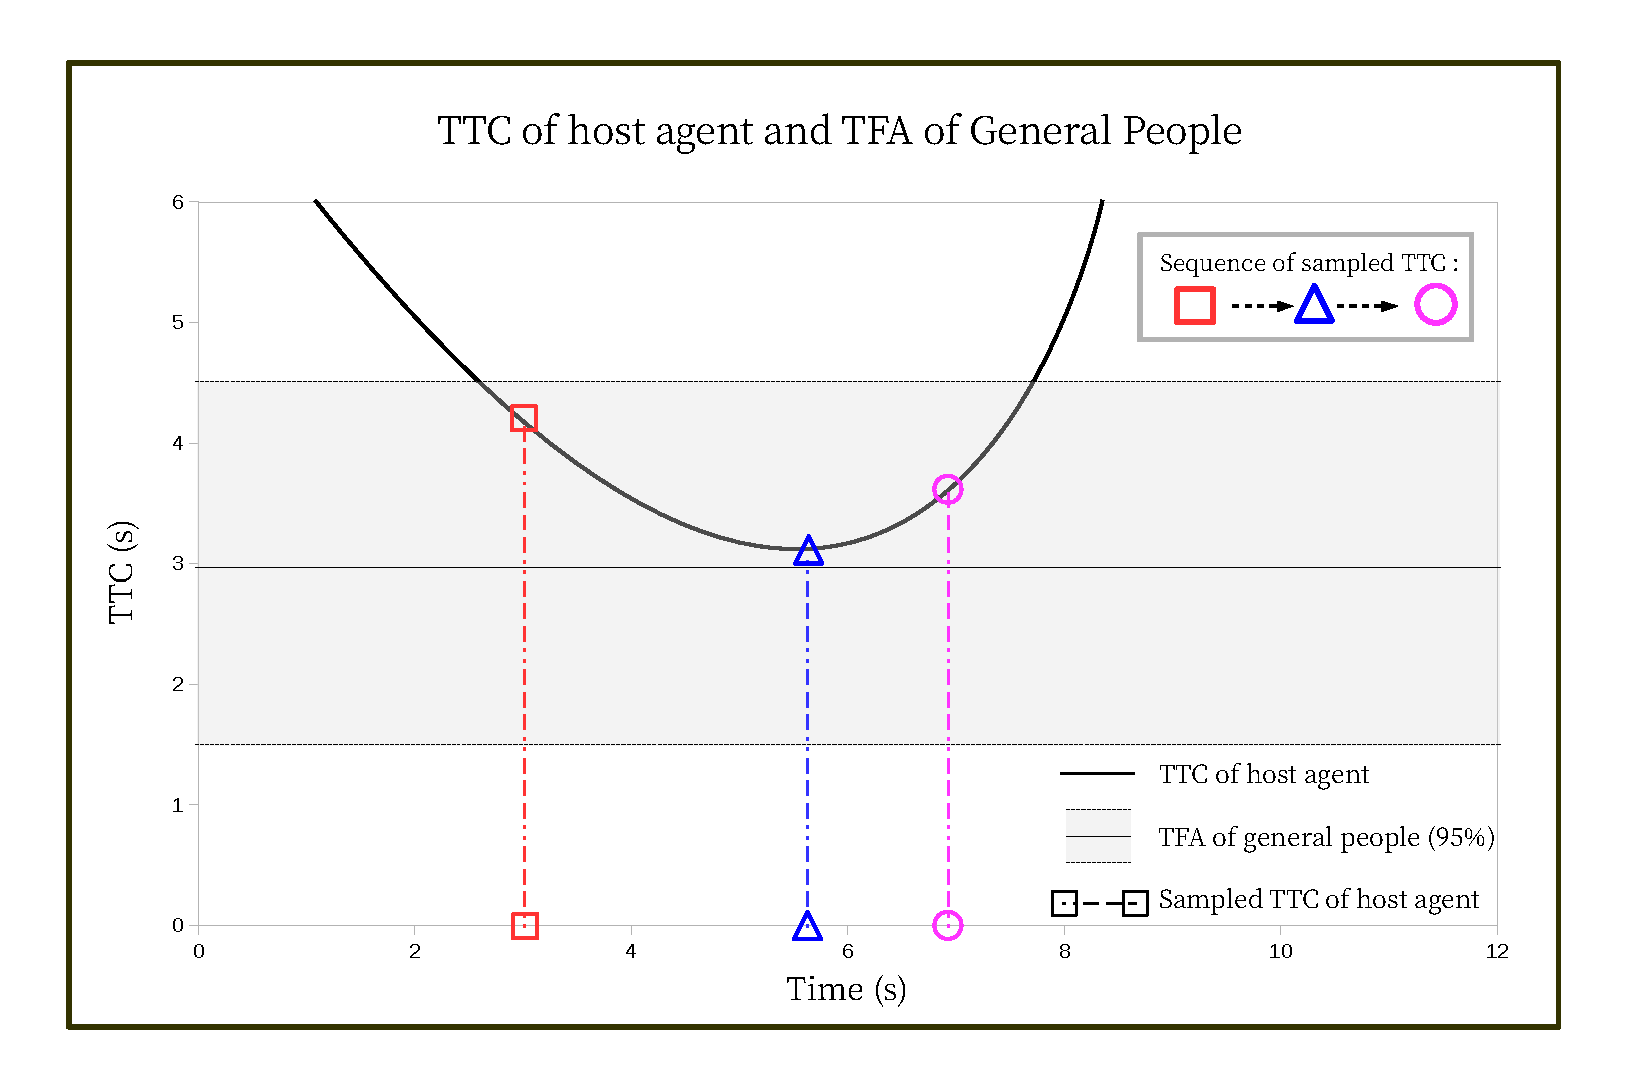
\includegraphics[scale=0.5]{TTC_probability_indicator.pdf}
\end{center}
\caption{Example of TFA of general people and TTC of the host agent.}
\label{fig:TTC_TFA_indicator} 
\end{figure}

\begin{figure}[htbp!]
\begin{center}
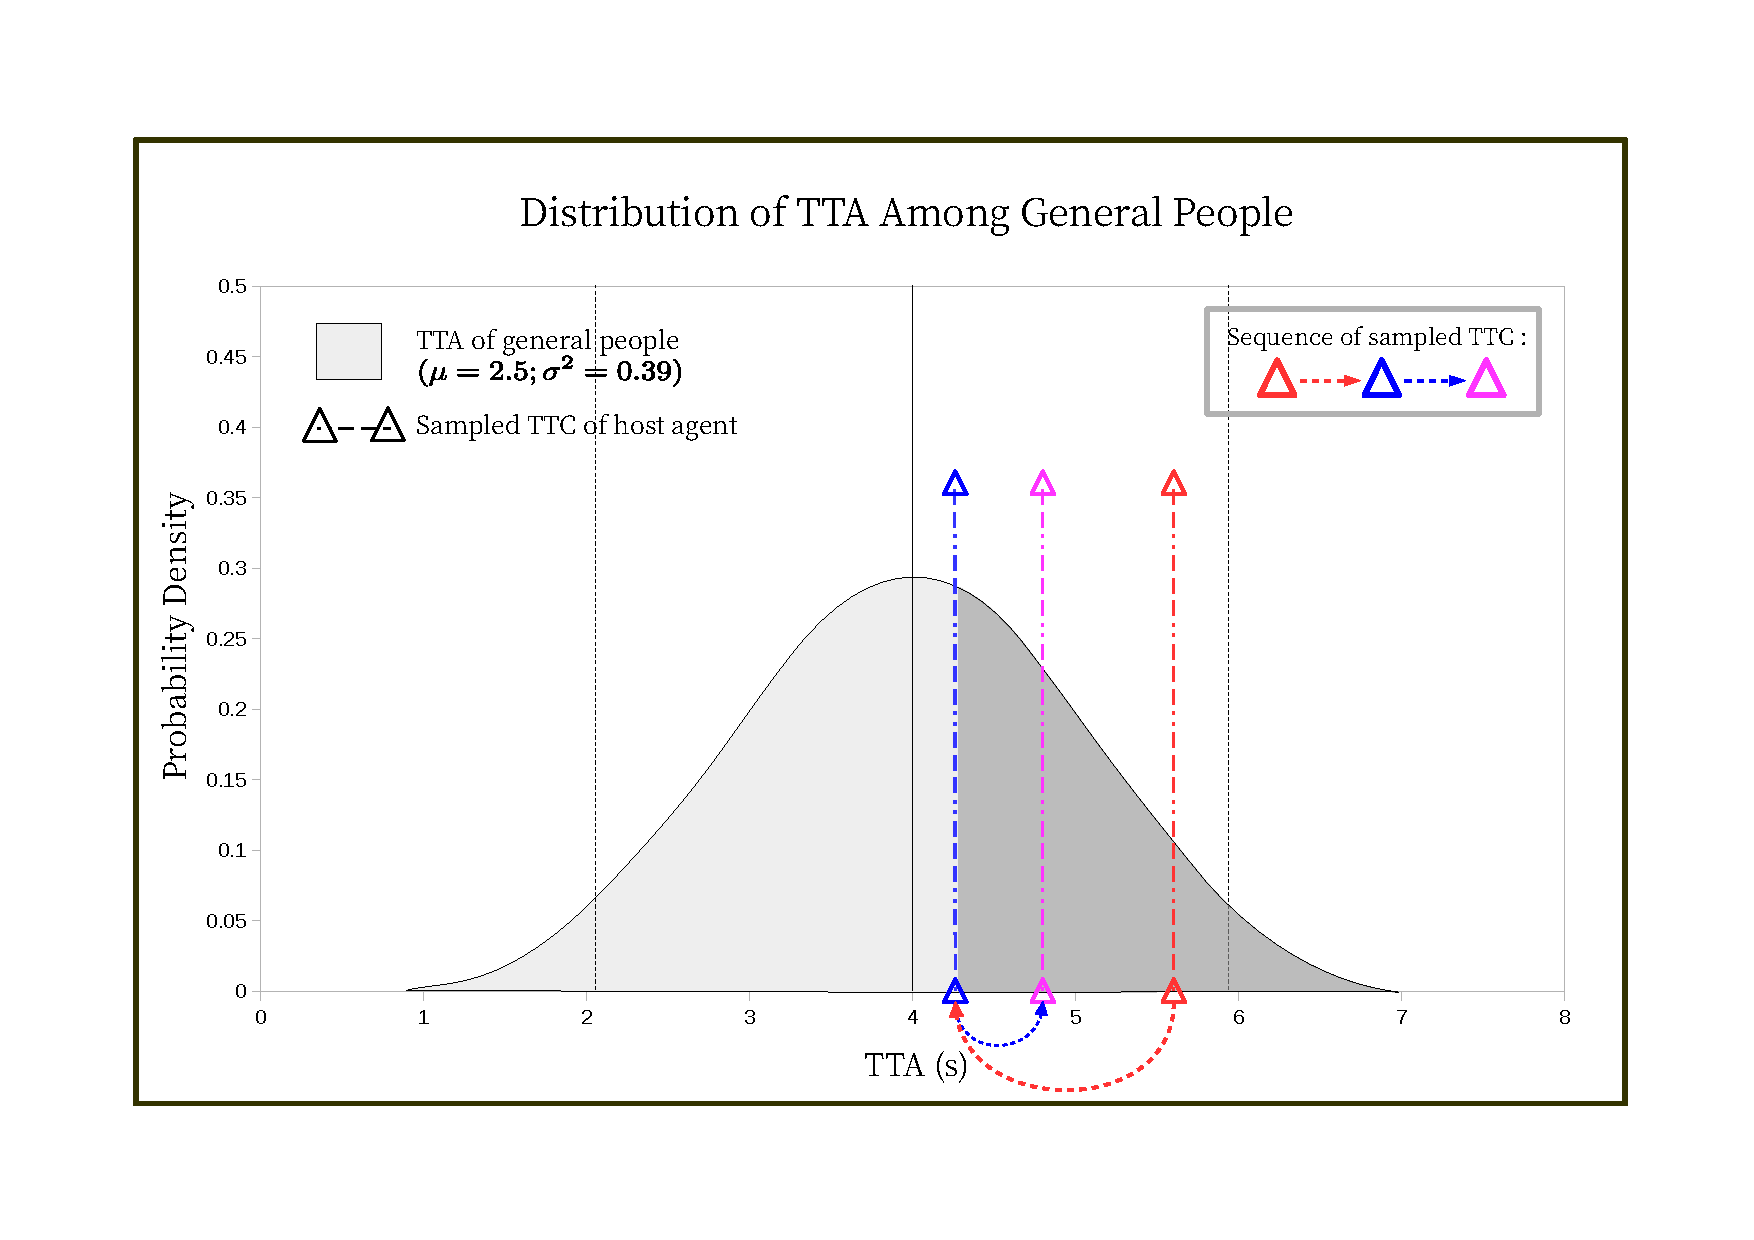
\includegraphics[scale=0.5]{TTC_probability_distribution.pdf}
\end{center}
\caption{Example of TFA distribution of general people.}
\label{fig:TTC_distribution} 
\end{figure}

So far we learned that the probability for the driver to brake is the integral of the PDF from the current, or the lowest in case the brake is applied, to the +inf. The probability to brake mentioned in the above paragraph refers to the intention that the driver brake to avoid potential obstacles. In the next section, the probability estimation method illustrated in this section will be used to evaluate the probability for the driver to yield to other traffic participants at the crossroad described in section \ref{sub:crossroad}.


%%%%%%%%%%%%%%%%%%%%%%%%%%%%%%%%%%%%%%%%%%%%%%%%%%%%%%%%%%%%%%%%%%%%%%%%
%%%%%%%%%%               SECTION SECTION SECTION               %%%%%%%%%
%%%%%%%%%%%%%%%%%%%%%%%%%%%%%%%%%%%%%%%%%%%%%%%%%%%%%%%%%%%%%%%%%%%%%%%%
\section{ Probability of Yielding}
\label{sec:POY}

To this moment, the probability for a driver to brake can be calculated using the PDF of TFA of general people, but merely integrating the PDF is still inadequate to explain the probability for the driver to yield. For example, assuming a driver drives towards the node without decelerating. Throughout the whole operation, the TTC of the host agent decreases, resulting the rising of the \ac{POY} (increasing area right to the current TTC and under the TFA distribution), which is a contradiction to our goal. Additionally, the TFA distribution for a driver is a function of the speed, hence the distribution Fig.~\ref{fig:TFA_distr_combined} represents the TFA distribution of general people (combined data of participants). In preparation for the driver yielding model at crossroads, firstly the TFA distribution model that can account for the distributions under different  speed is required, secondly parameters that are able to explain all possible circumstances should be included.   


%%%%%%%%------------------------------%%%%%%%%%
%%%%%%%%-----------SUBSECTION---------%%%%%%%%%
%%%%%%%%------------------------------%%%%%%%%%
\subsection{TFA Distribution Modeling}

In this work, we focus on the crossroad scenario described earlier where two drivers drive toward the node (the intersection of their courses) on the paths perpendicularly to each other at the same time. The term $\mathbf{d_{node,i, t}}$ in Eqn.~(\ref{eq:TTC_crossroad}) denotes the displacements to the node that change along with time. In other words, at the moment that the driver has the intention to yield, this term will then represent the distance required for the vehicle braking and keeping a distance between the vehicle and the node when fully stopped which is the \textit{distance left before action} in Fig.~\ref{fig:TFA_model} .

\begin{figure}[htbp!]
\begin{center}
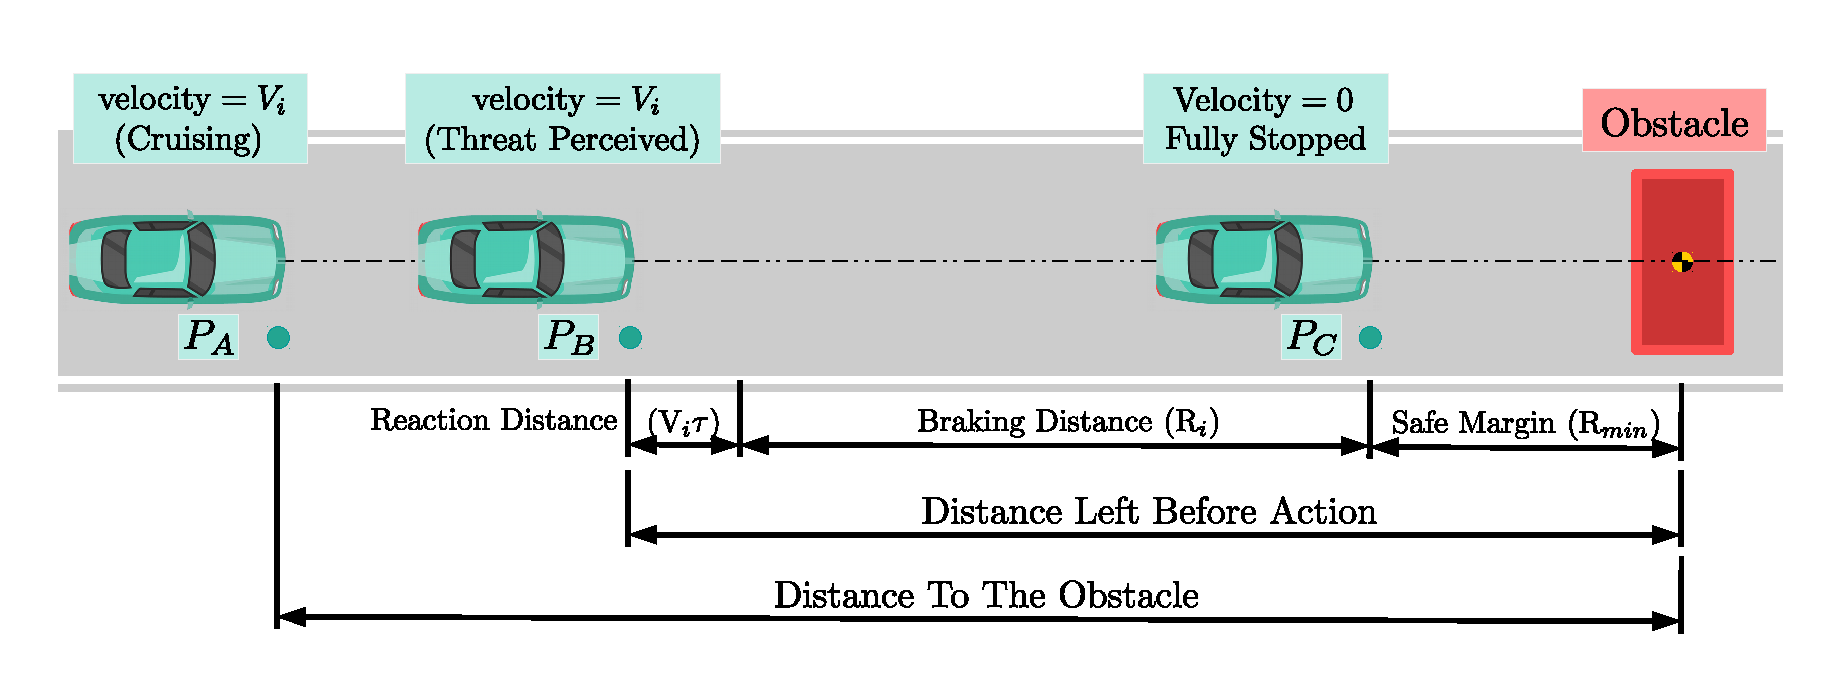
\includegraphics[scale=0.45]{TFA_TTC_model.pdf}
\end{center}
\caption{Decomposing the distance left before action (apply the brake).}
\label{fig:TFA_model} 
\end{figure}


The distance left before action is broken down into three parameters in Fig.~\ref{fig:TFA_model}, which are reaction time, braking distance and the safe margin (i.e. the distance left when fully stopped). The reaction time is the combination of the human perception-reaction delay and the vehicle actuation delay, i.e., these are the time that drivers need from seeing a potential threat to hitting the brake and the time the brake system need to decelerate the vehicle after the applying the brake. The braking distance stands for the distance the vehicle need to be fully stopped. And the safe margin is the distance left between the host vehicle and the obstacle when the vehicle is fully stopped. The reaction time can be expressed as 

\begin{equation}
\text{Reaction Time} = {v_i}\tau
\label{eq:V_tau}
\end{equation}

\noindent where ${v_i}$ is the speed of the subject vehicle at the very moment when the brake is applied and $\tau$ is the combination of system and driver delays as mentioned earlier. The second parameter is the braking distance, denoting as

\begin{equation}
R_{i} = \frac{v_i^2}{2a_{dec}}
\label{eq:R_i}
\end{equation}

where ${v_i}$ is same as the one in Eqn.~\ref{eq:V_tau} which stands for the speed of the vehicle at that moment while $a_{dec}$ represents the average deceleration applied during the braking. What should be noted here is that Eqn.~\ref{eq:R_i} is based on the assumption that the constant deceleration is applied throughout the entire braking process. The last parameter, safe margin, is denoted as $R_{min}$ which stands for the safe distance that the driver left after the vehicle is fully stopped. For the sake of making data extraction easier, the $R_{min}$ is defined as distance from the center of one vehicle to another. Combining these three parameters we have the distance left for braking as

\begin{equation}
\text{Distance Left Before Braking} = R_i+v_i\tau+R_{min}
\label{eq:TFA_distance}
\end{equation}

One should have been aware of the fact that the meaning of this distance is exactly the distance term in Eqn.~\ref{eq:TTC_crossroad} when the TTC at this moment equals the TFA of the driver, since Eqn.~\ref{eq:TFA_distance} is the estimated distance needed for the driver if he or she attempts to yield at this moment.  So dividing Eqn.~\ref{eq:TFA_distance} by the speed of the subject vehicle ${v_i}$ we will have

\begin{equation}
\text{TFA}_{est} = \frac{R_i+v_i\tau+R_{min}}{v_i} 
\label{eq:TFA_est}
\end{equation}


\noindent where ${TFA}_{est}$ represents the estimated TFA of the driver. This ${TFA}_{est}$ is then applied as the mean value of the TFA distribution under the vehicle speed ${v_i}$. Combining all the element, the TFA distribution is now described as


\begin{equation}
\text{TFA} \sim \mathcal{N}(\text{TFA}_{est},\,\sigma_{est}^{2})\,.
\label{eq:TFA_distribution}
\end{equation}

and the value of the variance $\sigma^2$ is defined as 

\begin{equation}
\sigma_{est} = \gamma \cdot \text{TFA}_{est}
\label{eq:TFA_distribution}
\end{equation}

\noindent where $\gamma$ is the coefficient for standard deviation, which is obtained from the ratio of $\mu$ and $\sigma$ obtained from the approximated normal distribution of TFA. 

As mentioned in Section \ref{sub:TFA Distribution}, the TFA distribution is suggested to vary under different velocity. It seems more plausible using the TFA distribution described in Eqn.~\ref{eq:TFA_est}. To confirm this idea, the experiments similar to the one conducted in Section \ref{sub:TFA Distribution}( to prove the TFA distribution is normally distributed ) is repeated but under different velocity at the moment of the brake. The velocity varies from 2.5 to 5 m/s using 0.5 as the step. Results of two participants are shown in Fig~.\ref{fig:Par1TFADifSpeed} and Fig~.\ref{fig:Par3TFADifSpeed}.

\begin{figure}[htbp!]
\begin{center}
\makebox[0pt]{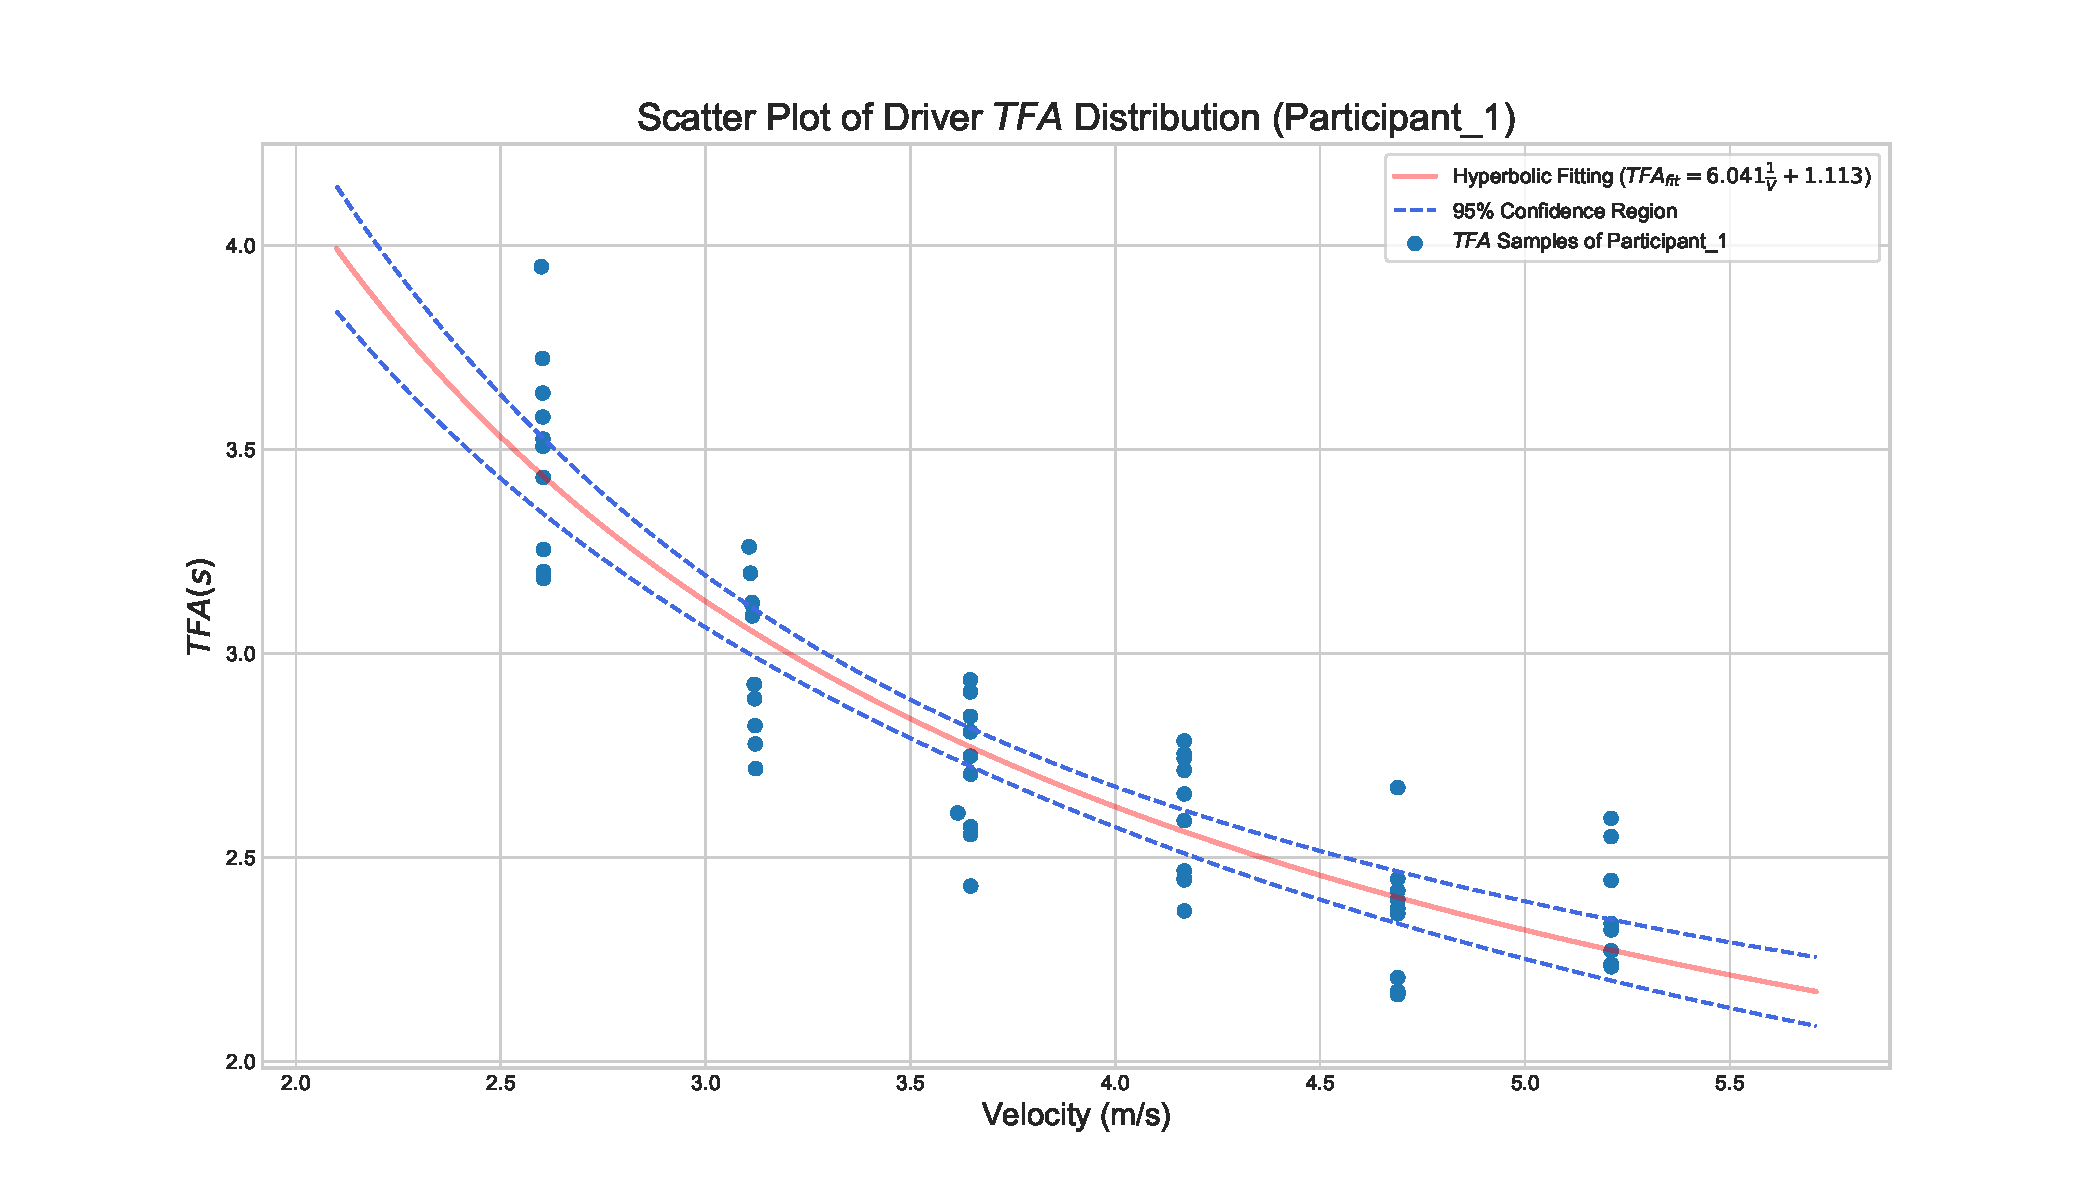
\includegraphics[width=0.7\paperwidth]{/Participant_1_TFA_polyfit.pdf}}
\end{center}
\caption{The TFA scatter plot of Participant 1 under various velocities.}
\label{fig:Par1TFADifSpeed} 
\end{figure}

\begin{figure}[htbp!]
\begin{center}
\makebox[0pt]{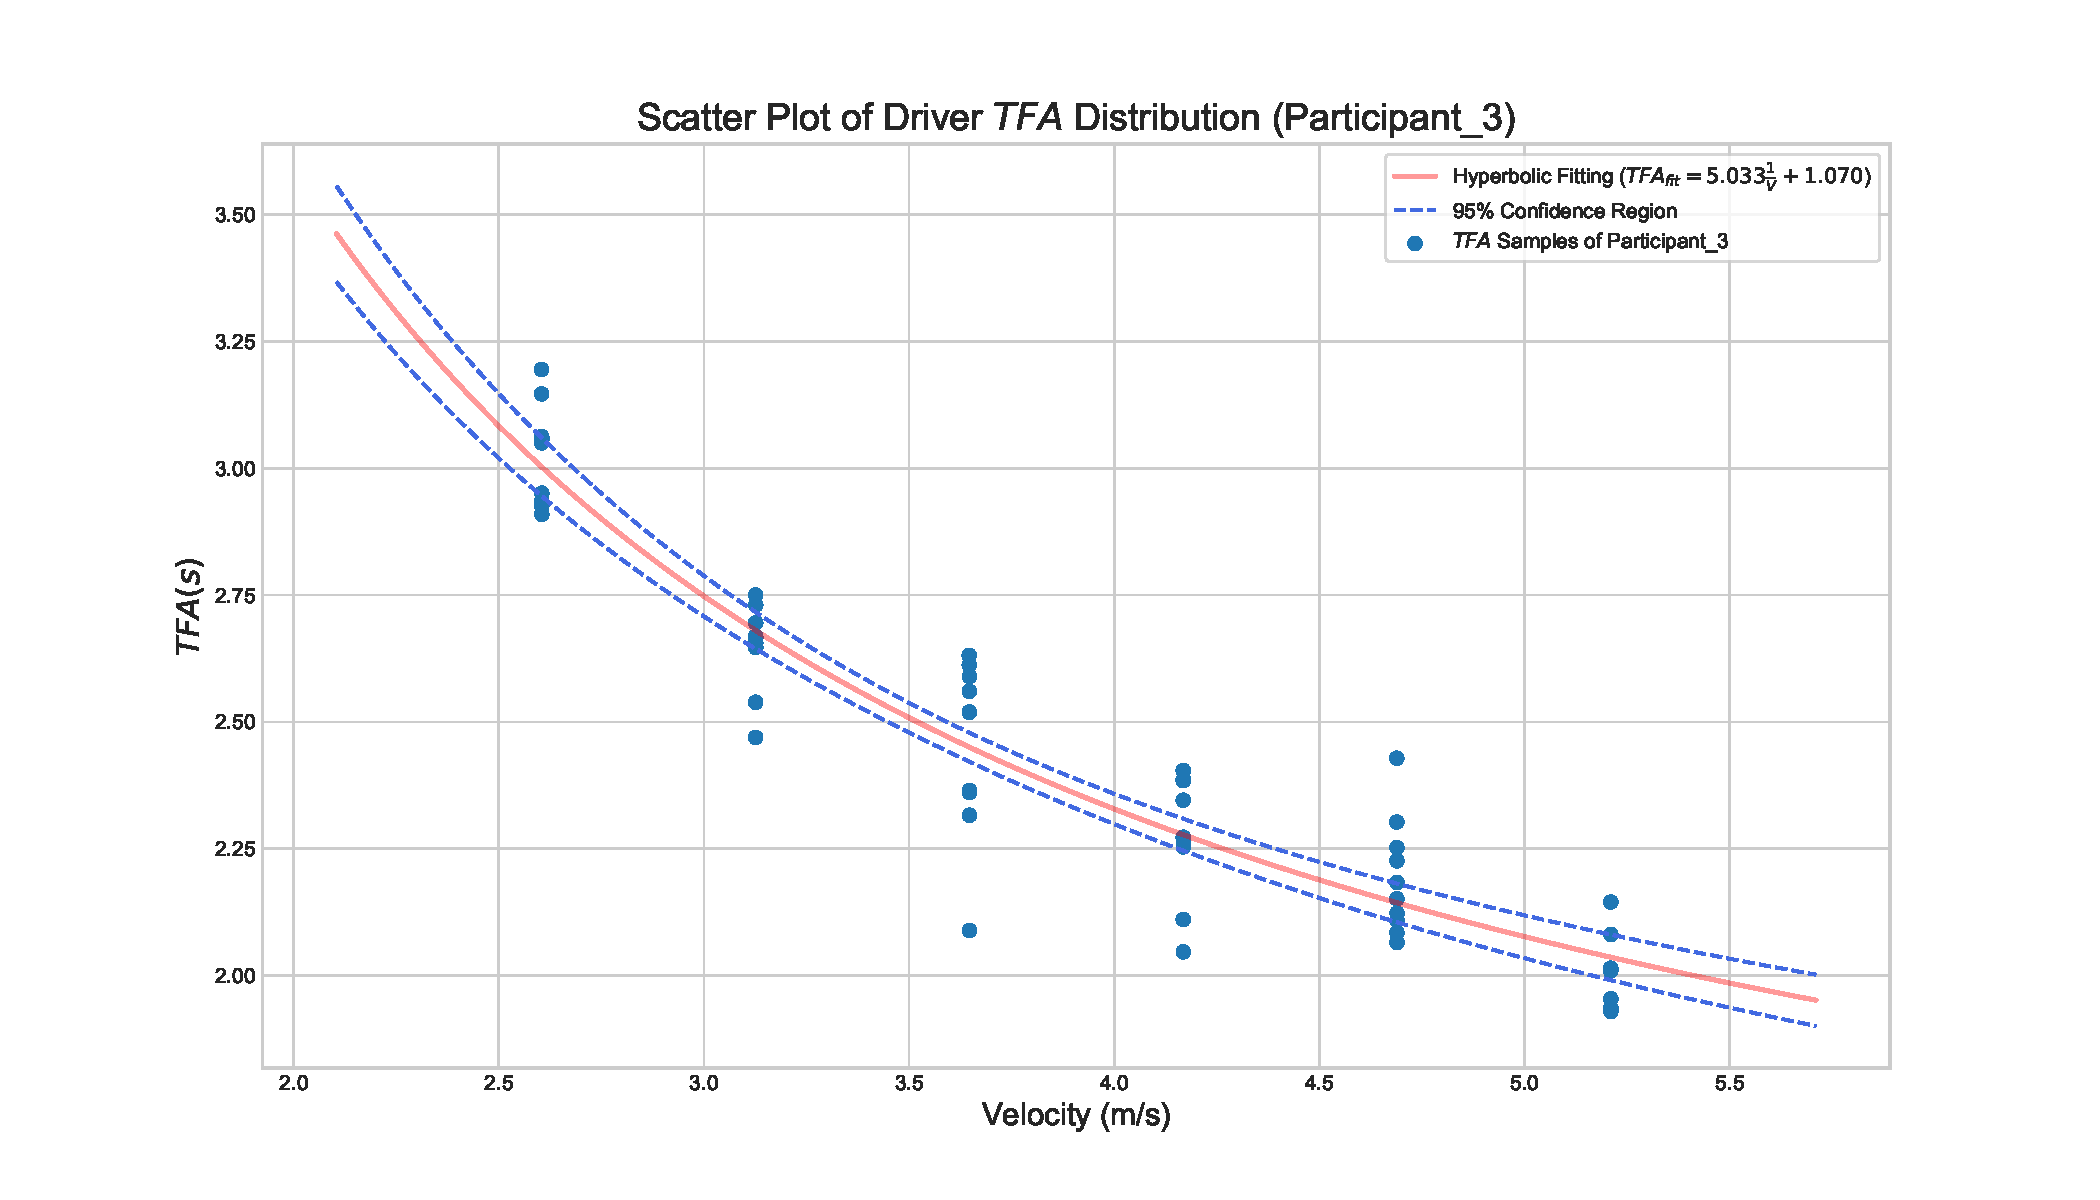
\includegraphics[width=0.7\paperwidth]{/Participant_3_TFA_polyfit.pdf}}
\end{center}
\caption{The TFA scatter plot of Participant 3 under various velocities.}
\label{fig:Par3TFADifSpeed} 
\end{figure}

In Fig~.\ref{fig:Par1TFADifSpeed} and Fig~.\ref{fig:Par3TFADifSpeed}, the blue dots are the collected data while the red line represents the curve fitting using hyperbolic equation. The reason for choosing hyperbolic equation is to provide evidence of how accurate the proposed $TFA_{est}$ equation is. It turns out that the TFA varies under different velocity following the hyperbolic equation, which is similar to the relation in Eqn.~\ref{eq:TFA_est}.

Now the ${TFA}_{est}$ is identified to be a function of ${v_i}$ as described in Eqn.~\ref{eq:TFA_est}, there are only three parameters left to be identified before completing the TFA distribution model. Since $\tau$ represents the reaction time of the driver which is biological trait, it can be considered as a constant under different speed. $R_{min}$ and $a_{dec}$ on the other hand, are functions of velocity due to different possible consequences at different velocities. For instance, people might have more aggressive actions when at lower speed (e.g. smaller $R_{min}$ for closer distance to the other vehicle after stopped) since everything is under control (i.e. the severity of the collision is low). While at high speed, however, drivers tend to act more conservatively (e.g. larger $R_{min}$ to keep a "safer margin") to avoid the serious collision. Experiments are conducted and shown to confirm the idea.

To estimate the parameters needed for TFA distribution of average drivers, data collected from participants are combined and analyzed in Fig.~\ref{fig:CombRMINDifSpeed} and Fig.~\ref{fig:CombADECDifSpeed}. The corresponding linear equation defining $R_{min}$ and $a_{dec}$ under various velocity are also presented.

\begin{figure}[htbp!]
\begin{center}
\makebox[0pt]{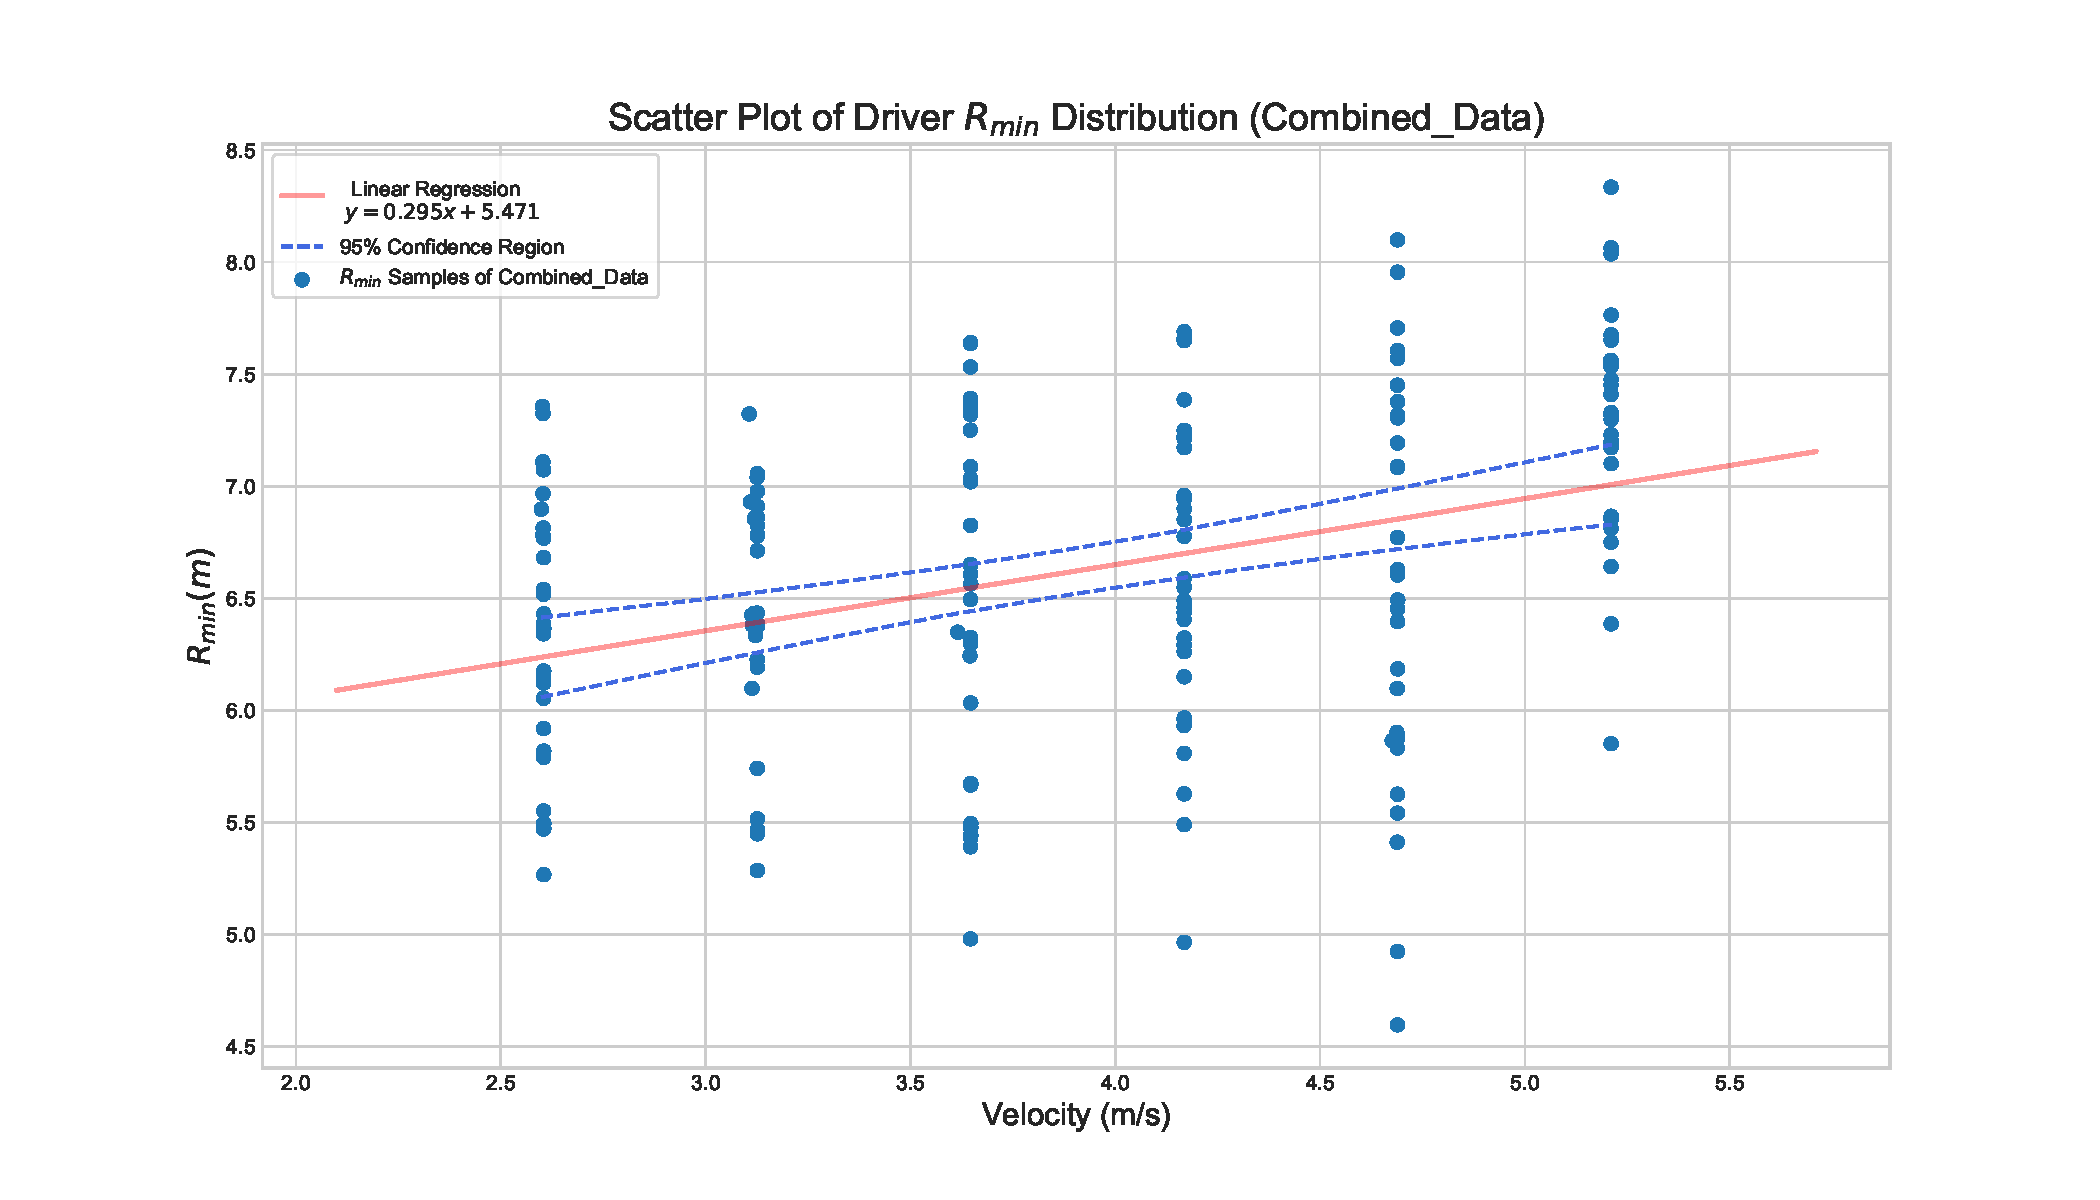
\includegraphics[width=0.7\paperwidth]{Combined_Data_R_MIN_polyfit.pdf}}
\end{center}
\caption{The $R_{min}$ scatter plot of combined data under various velocities.}
\label{fig:CombRMINDifSpeed} 
\end{figure}

\begin{figure}[htbp!]
\begin{center}
\makebox[0pt]{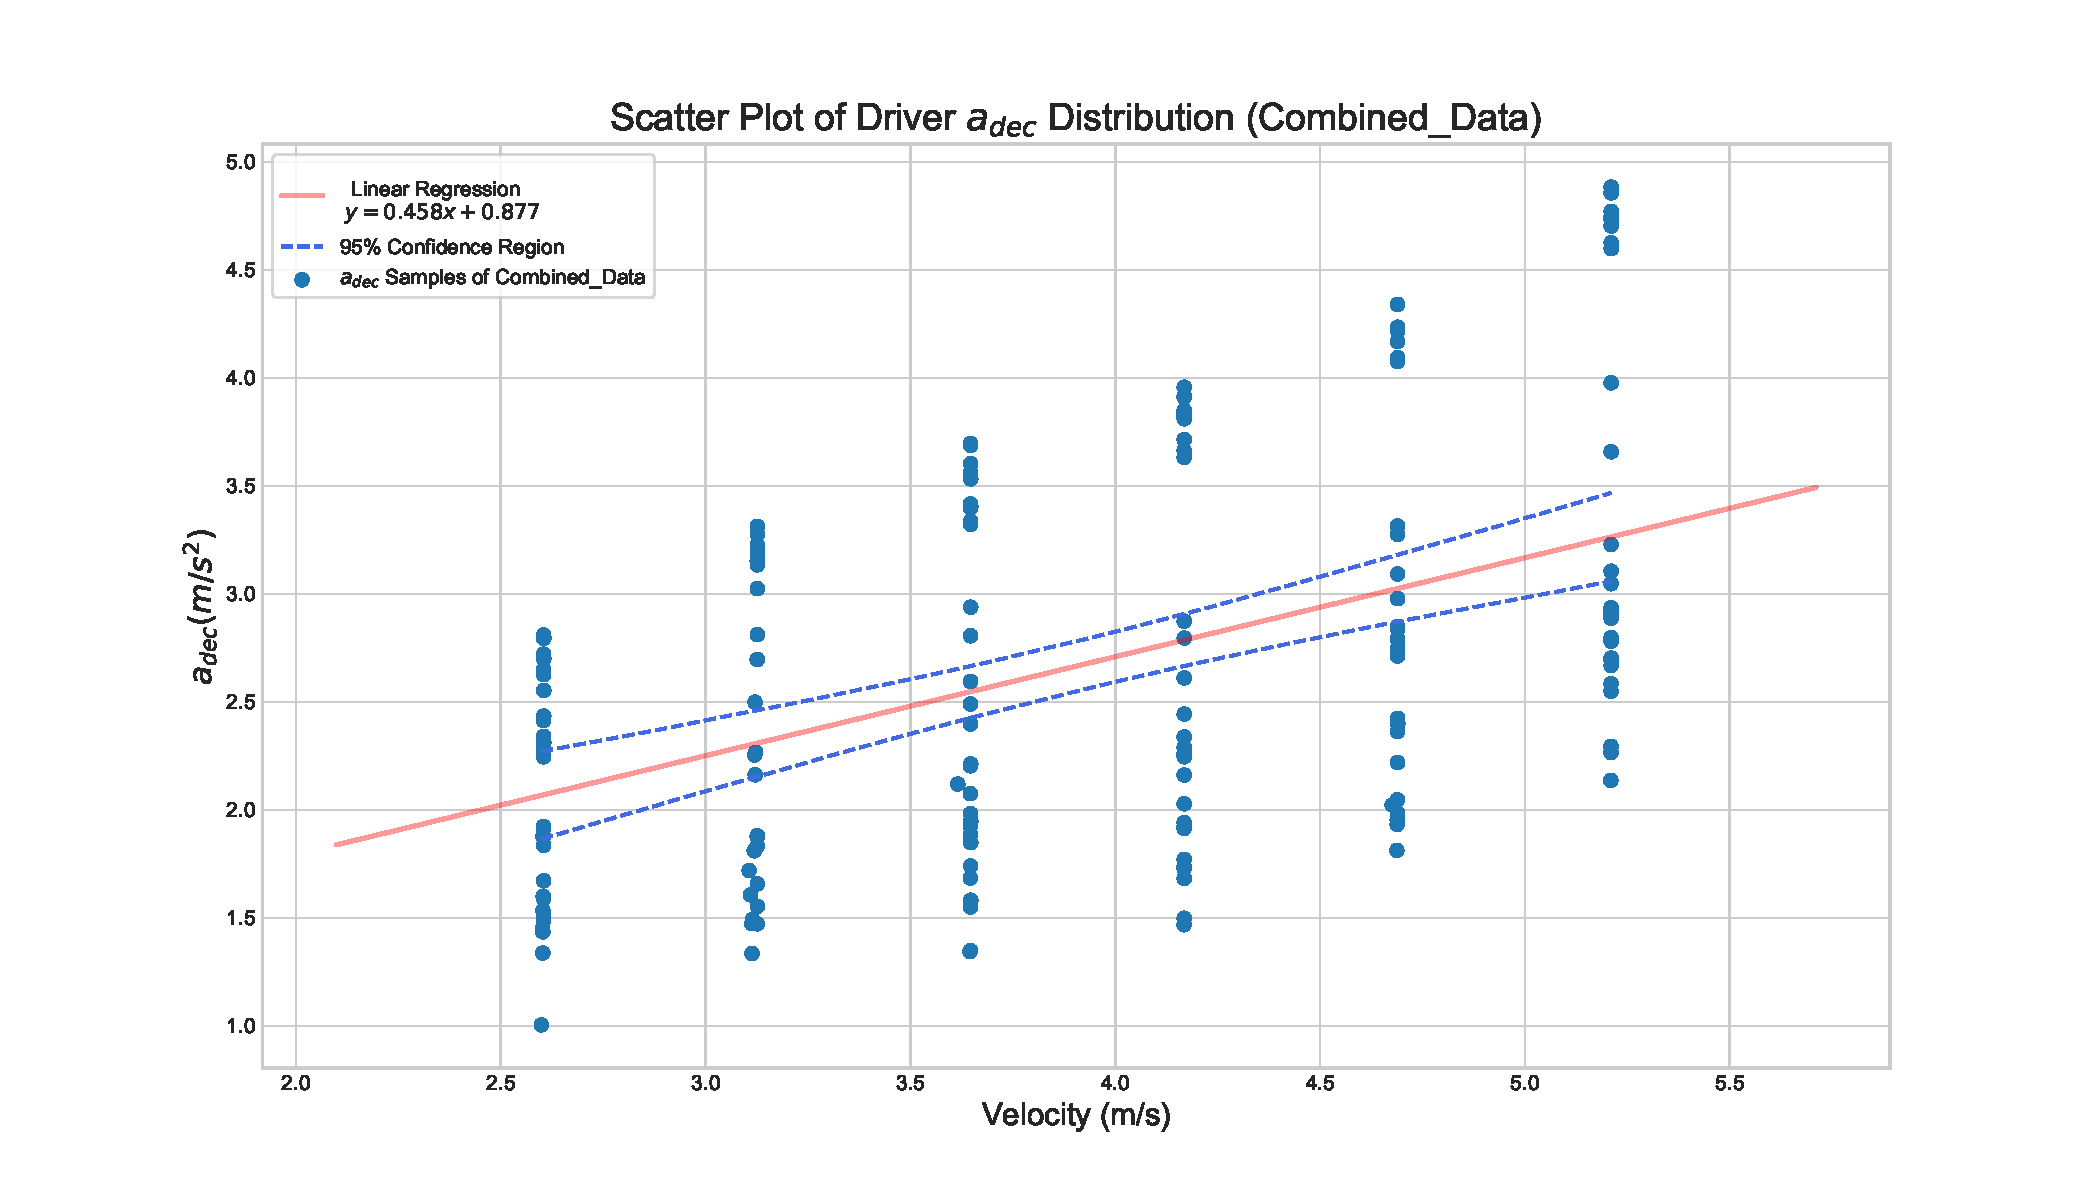
\includegraphics[width=0.7\paperwidth]{Combined_Data_A_DEC_polyfit.pdf}}
\end{center}
\caption{The $a_{dec}$ scatter plot of combined data under various velocities.}
\label{fig:CombADECDifSpeed} 
\end{figure}

\noindent where the approximated  equations for $R_{MIN}$ and $a_{dec}$ are

\begin{equation}
R_{min} = 0.295 v_i + 5.471
\label{eq:RMIN_Linear}
\end{equation}

\begin{equation}
a_{dec} = 0.458 v_i + 0.877
\label{eq:ADEC_Linear}
\end{equation}


We can see that the $R_{min}$ does get higher linearly as the velocity rises which is the same as predicted. The same trends happen to the $a_{dec}$ as the velocity ascends, which suggests that drivers brake slowly at low velocity and rapidly at high velocity. This is also reasonable since more urgent the situation is when the velocity is high. Therefore, the $R_{min}$ and $a_{dec}$ in Eqn.~\ref{eq:TFA_est} are also functions of $v_i$ which can be approximated by linear equation. Now we have all the elements needed, the required TFA distribution under different speed can now be estimated using ${TFA}_{est}$. Parameters used in the proposed TFA distribution estimation are listed in Table~\ref{table:parameters}. 

\begin{table}[htbp]
\caption{Table for parameters used in TFA distribution model.}
\begin{center}
\label{table:parameters}
\begin{tabular}{l l l l c}
& & \\ % put some space after the caption
\hline
\textbf{Parameters} &  & & &\textbf{Values} \\
\hline
Safe Margin Coefficient (${C1}_{Rmin}$)     &  &  & &  0.295  \\
Safe Margin Constant (${C2}_{Rmin}$)     &  &  & &  5.471  \\
Deceleration Coefficient (${C1}_{adec}$) &  &  & & 0.458  \\
Deceleration Constant (${C2}_{adec}$) &  &  & & 0.877  \\
Reaction Time ($\tau$)        &  &  & & 0.6 $s$ \\
Standard Diviation Parameter ($\gamma$)      &  &  & & 0.148  \\
\hline
\end{tabular}
\end{center}
\end{table}

\noindent where Safe Margin Coefficient (${C1}_{Rmin}$), Safe Margin Constant (${C2}_{Rmin}$), Deceleration Coefficient (${C1}_{adec}$), and Deceleration Constant (${C2}_{adec}$) standing for the coefficients and constants of the linear equation of $R_{min}$ and $a_{dec}$. $R_{min}$ and $a_{dec}$ are formulated in Eqn.~\ref{eq:RMIN_Linear} and Eqn.~\ref{eq:ADEC_Linear}.

\begin{equation}
R_{min} = {C1}_{Rmin} v_i + {C2}_{Rmin}
\label{eq:RMIN_Linear}
\end{equation}

\begin{equation}
a_{dec} = {C1}_{adec} v_i + {C2}_{adec}
\label{eq:ADEC_Linear}
\end{equation}

Finally, the model to estimate the TFA distribution of general people is completed. The TFA distributions are proved to be normally distributed and the formulated $TFA_{est}$ can also account for the hyperbolic growth in the TFA data collected. In the next section, the TFA distribution will be used as the core of the proposed probabilistic model.

%%%%%%%%------------------------------%%%%%%%%%
%%%%%%%%-----------SUBSECTION---------%%%%%%%%%
%%%%%%%%------------------------------%%%%%%%%%
\subsection{The Model for Probability of Yielding Estimation}
So far, the problem concerning the model for TFA distribution is solved by considering the distance needed for the driver to yield. Then the distance is divided by the speed at the instance and turned into the ${TFA}_{est}$. Before the TFA distribution is brought into the probability evaluation method proposed in section \ref{sub:TFA PDF}, few improvements are required because the proposed model is unable to account for all the situations yet. 

For example, the situation where a vehicle is accelerating through the node is described in Fig.~\ref{fig:TTC_acc}. Three sub-figure from the top to the bottom are the velocity, the displacement to the node and the TTC versus the time respectively. Note that in this example, the acceleration of the vehicle is constant, so the line of velocity rise linearly while the displacement to the node and TTC are a parabolic and the curve consisting of reciprocal and linear function separately. In this figure, as the velocity of the vehicle is accumulating, the displacement to the node drops in a parabolic curve since the vehicle is moving closer. The resulting TTC curve, defined by Eqn.~\ref{eq:TTC_crossroad}, is also decreasing and even goes beneath 0. In the cases like this one, the POY using merely the integral from the TFA distribution, as in Fig.~\ref{fig:TTC_distribution}, would causing the increase of the POY as the TTC keeps decreasing.

\begin{figure}[htbp!]
\begin{center}
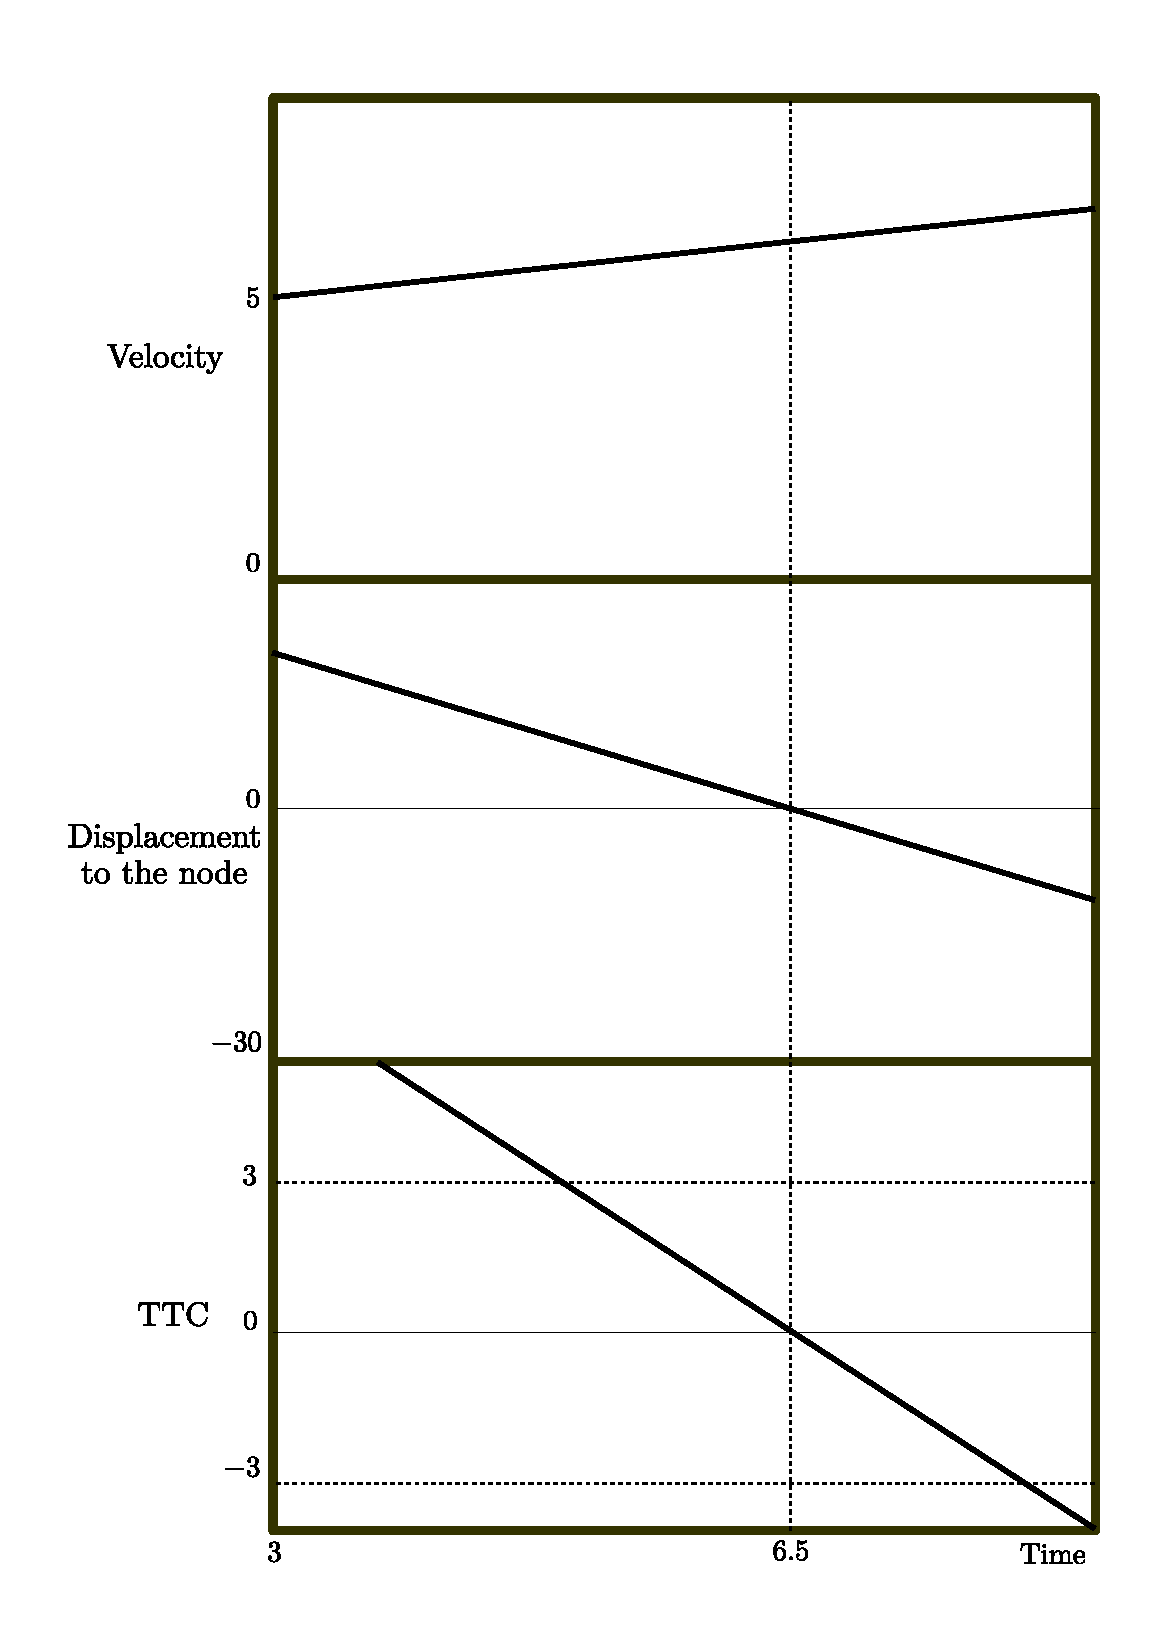
\includegraphics[scale=0.6]{TTC_change_when_accelerating.pdf}
\end{center}
\caption{History of TTC as the vehicle accelerating through the node.}
\label{fig:TTC_acc} 
\end{figure}

To overcome this problem, few adjustments are needed to be performed. First, the influence of the acceleration on the probability of stopping should be considered. As described in the above example, besides the integral acquired from the TFA distribution, the current states of acceleration are also important. After some trials for different possibilities, the first order derivative of TTC is chosen. By assuming constant acceleration while braking, the $d_{node, i, t}$ can be expressed as

\begin{equation}
d_{node, i, t} = d_{node,i,0} - \biggl(v_0t+\frac{1}{2}at^2\biggr)
\label{eq:d_node}
\end{equation}

\noindent where $d_{node,i,0}$ is the displacement at the beginning of the brake, $v_0$ is the speed and $a$ the acceleration. Then, combining Eqn.~\ref{eq:d_node} and Eqn.~\ref{eq:TTC_crossroad}, the derivative of TTC is determined

\begin{equation}
TTC' = \frac{d}{dt}\frac{d_{node,i,t}}{v_t} = -1 -a \cdot d_{node,i,t} \cdot v_t^{-2}
\label{eq:TTC'}
\end{equation}

As a dimensionless weighting parameter, $TTC'$ takes not only acceleration but also displacement and the speed into account. For instance, when a constant deceleration is applied, the higher the speed of the vehicle implies the smaller chance this vehicle will yield and vice versa. So this weighting parameter is capable of punishing those with low TTC while accelerating or at high speed and rewarding those with deceleration or low speed. Now, the last step is to add this weighting on the proposed model. 

In order to increase the POY in those circumstances such as the deceleration or the low vehicle speed, the mean value of ${TFA}_{est}$ should is elevated. Similarly, to decrease the POY while the vehicle is accelerating or driving with high speed, the mean value of ${TFA}_{est}$ is reduced. However, chances are the brake is not applied to yield but to adjust the speed, or it is not acceleration but simply some sensor errors, which all could lead to bumpy probabilities of yielding. To bring down the number of the results affected by false positive, the following adjustments are made


\begin{equation}
    P_{yield, t} = \Bigr(1-\Phi_{\mu, \sigma^{2}}\big({min TTC}_{t}\big)\Bigl)
\label{eq:POY}
\end{equation}

where  $P_{yield, t}$ is the proposed probability of yielding at time $t$, $\Phi_{\mu, \sigma^{2}}$ is the CDF of the TFA distribution $\mathcal{N}(\mu,\sigma^{2})$, $\mu$ is defined by ${TFA}_{est, t} + A_{t}$ which represents the adjusted mean value of the TFA distribution and $\sigma_{est, t}$ is the resulting adjusted mean value of the TFA distribution.

The weighting parameter $A_{t}$ is defined as

\begin{equation}
    A_{t} = 
    \begin{cases} 
      \alpha_{t} &~~\text{if}~~ \lvert \alpha - \alpha_{t-1}  \rvert < 1.67 \cdot \sigma_{est, t}\\
      1.67 \cdot \sigma_{est, t} &~~\text{otherwise}
    \end{cases}
\label{eq:alpha_cap}
\end{equation}

\noindent where $\alpha_t$ in Eqn.~\ref{eq:alpha_cap} is dominated by the acceleration. From Eqn.~\ref{eq:TTC'}, we can see that the $TTC'$ equals -1 when the acceleration is 0. So the $TTC'$ value is greater than -1 when the subject vehicle is decelerating, and less than -1 when accelerating. In order to account for the acceleration as well as the velocity, $\alpha_t$ is defined as 

\begin{equation}
    \alpha_{t} = 
    \begin{cases} 
      \beta_{t} \cdot \ln \left ( ~ \left( ~ \lvert {TTC'}_{t}  \rvert + 1 ~\right) \cdot e~ \right) &~~\text{if}~~ {TTC'}_{t} > -1\\
      - \beta_{t} \cdot \ln \left ( ~ \left( \lvert {TTC'}_{t}  \rvert + 1 \right) \cdot e~ \right) &~~\text{if}~~ {TTC'}_{t} < -1 \\
      \alpha_{t-1} &~~\text{otherwise}
    \end{cases}
\label{eq:alpha}
\end{equation}

\noindent where

\begin{equation}
    \beta_{t} = 
     \max ~ \big( ~ \lvert {min TTC}_{t} - TFA_{est, t} \rvert, ~ \sigma_{est, t} ~ \big)
\label{eq:beta}
\end{equation}



As describe in Eqn.~\ref{eq:POY}, the weighting $A_t$ is applied to increase the mean value of the TFA distribution. When the $A_t$ is positive, meaning that the POY will increase under the same TTC, which is due to the larger integral of that area under TFA distribution, and vice versa for the negative $A_t$ valaues. This is illustrated in Fig.~\ref{fig:TFA_weighting_before} and Fig.~\ref{fig:TFA_weighting_after}. In Fig.~\ref{fig:TFA_weighting_before}, the current TTC equals the mean of the TFA distribution so the resulting POY is 0.5 . However, since the vehicle is decelerating, the mean value of the TFA distribution is adjusted according to Eqn.~\ref{eq:alpha}. The POY, which is the area under the TFA distribution and right to the current TTC, becomes 0.97, as illustrated in Fig.~\ref{fig:TFA_weighting_after}.

\begin{figure}[htbp!]
\begin{center}
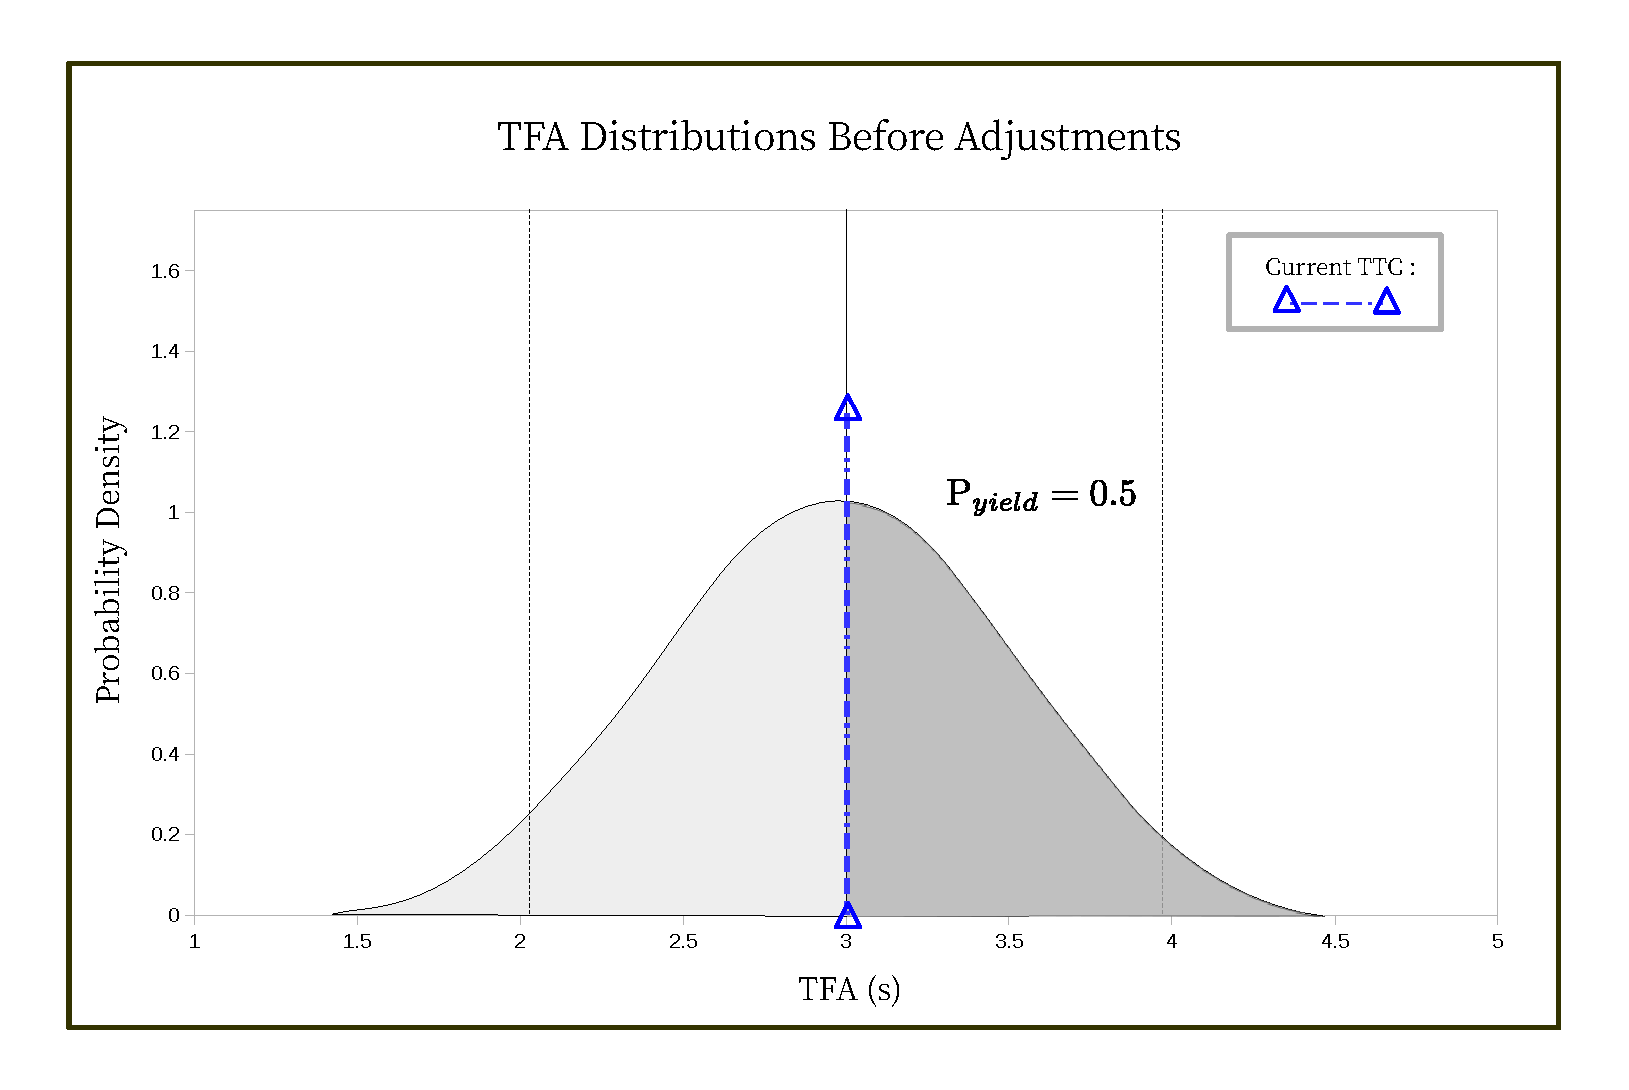
\includegraphics[scale=0.4]{TFA_weighting_before.pdf}
\end{center}
\caption{The probability before the weighting parameter $A_t$ is 0.5 .}
\label{fig:TFA_weighting_before} 
\end{figure}

\begin{figure}[htbp!]
\begin{center}
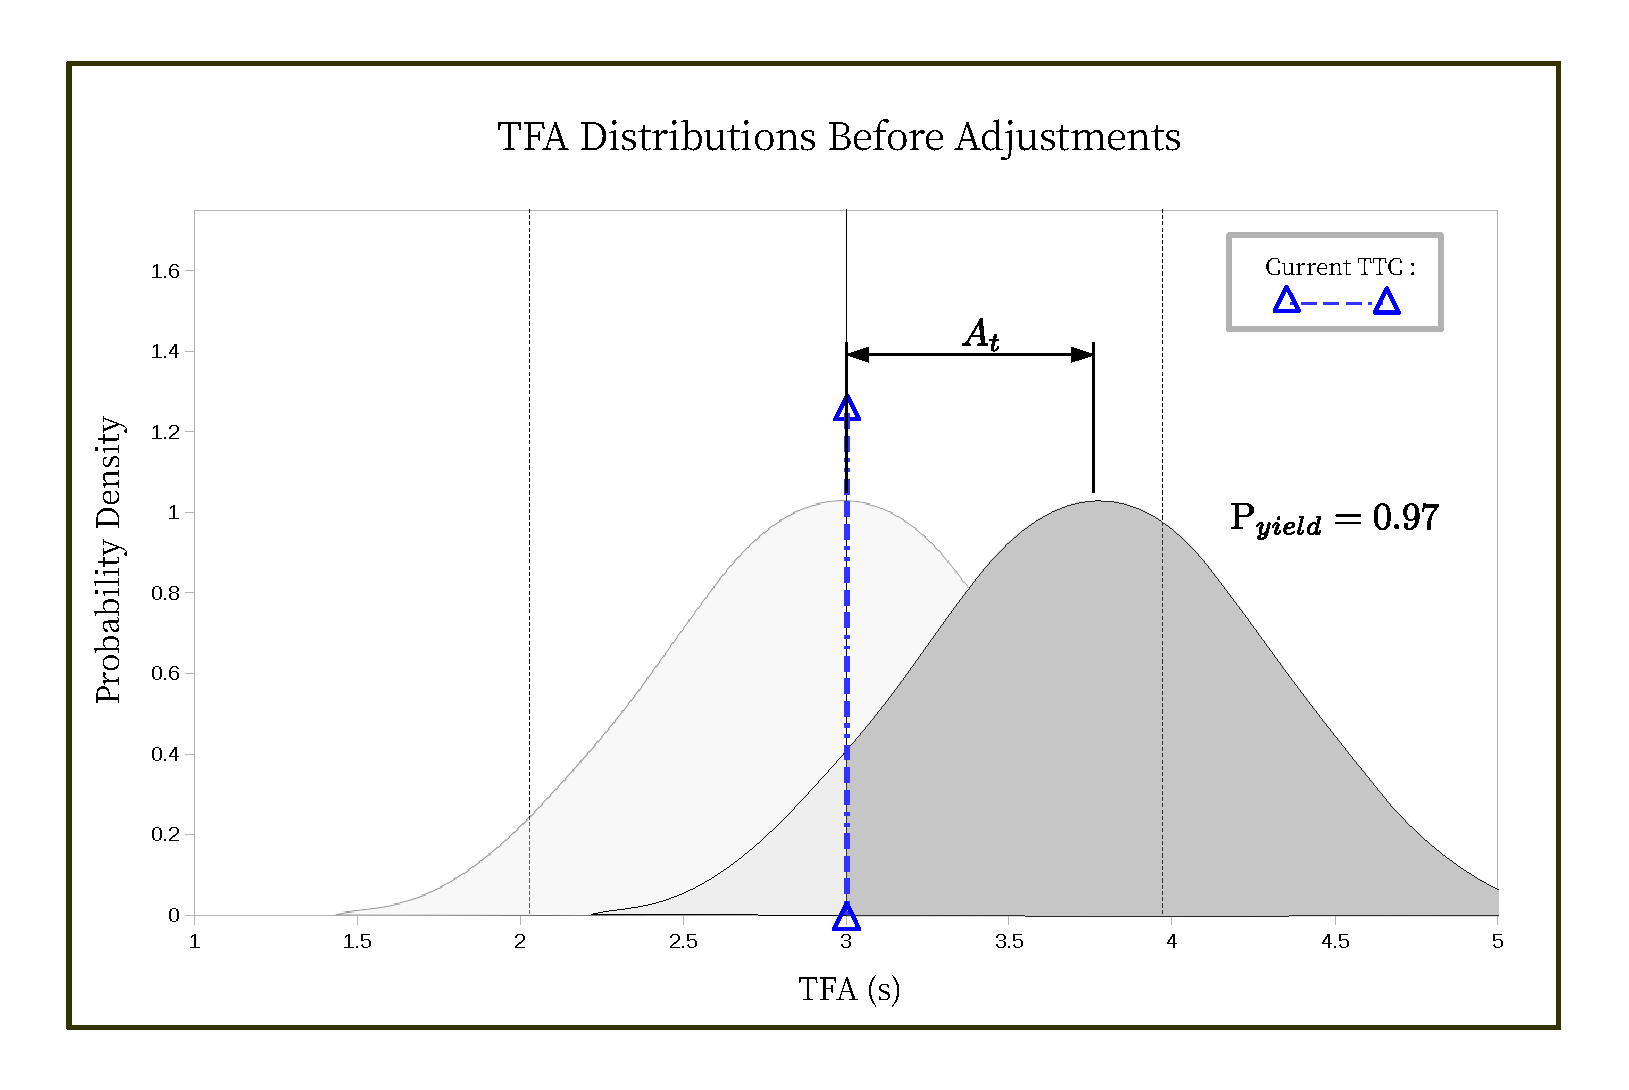
\includegraphics[scale=0.4]{TFA_weighting_after.pdf}
\end{center}
\caption{The probability after the weighting parameter $A_t$ is 0.97 .}
\label{fig:TFA_weighting_after} 
\end{figure}

In Eqn.~\ref{eq:alpha}, the magnitude of $\alpha_t$ is adjusted depending on the greater one between $\lvert {min TTC}_{t} - TFA_{est, t} \rvert $ and $ \sigma_{est, t}$ (as shown in Eqn.~\ref{eq:beta}). By doing so, the increase or decrease of the mean value of the TFA distribution will be in direct proportion to the difference between ${min TTC}_{t}$ and $TFA_{est, t}$ if $\lvert {min TTC}_{t} - TFA_{est, t} \rvert $ is larger. Within those situation where the $\lvert {min TTC}_{t} - TFA_{est, t} \rvert $ is too small or even equals to 0, $ \sigma_{est, t}$ is used instead. Either way, the resulting $\beta_{t}$ value allows the proposed model to have more immediate response to the situation at the moment. ( Noted that in Eqn.~\ref{eq:alpha}, $\lvert {TTC'}_{t} \rvert$ in both conditions are added by 1 and times $e$, so the outcome of the natural logarithm will be greater than 1 at all times. )

However, jagged POY curve might be shown if the response is "too immediate", in other word, if the value of $\alpha_t$ is too large, the resulting POY curve would be too cluttered. For example, if the current POY is 0.97 as depicted in Fig.~\ref{fig:TFA_weighting_after}, and the $\alpha_t$ at the moment is minus four standard deviation. In the next moment, the POY then drop rapidly from 0.97 to 0.0 . If situations like this keep repeating, there will be too many spikes for people to understand the real intention of the other driver. As a result, the maximum value of $A_t$ is set to 1.67 standard deviation to suppress the value and prevent the POY from rising or dropping too rapidly.  

Another reason for spikes on the POY curves is that, the throttles or brakes are sometimes applied for speed adjustments, not yielding or passing. To prevent the POY curve from making response to situations like this, the change of sign in $A_t$ would only be accepted when the acceleration introducing the change last for longer than 0.2 sec, i.e., when the vehicle starts braking, the $A_t$ brought by this brake would only be applied when the deceleration lasts longer than 0.2 sec. Even though the sensitivity to the yielding or passing cases might be diminished if the threshold is set too large, this can effectively reduce the number of cases falsely detected as the other intention. 

Up till now, the driver behaviors at the crossroad is modeled in a probabilistic way. The proposed probabilistic of yielding is able to anticipate the decision of drivers at the crossroad. With this functionality, the proposed method can help autonomous vehicle to understand the intentions of other traffic participants and make the mixed-fleet safer before the fully autonomous vehicles are adopted by 100\%.

The intents of drivers at simulated and real crossroad are predicted and shown using the proposed model. Then, the verification is conducted using the classification accuracy rate, and the results are also compared with other methods from the literature. 


%%%%%%%%%%%%%%%%%%%%%%%%%%%%%%%%%%%%%%%%%%%%%%%%%%%%%%%%%%%%%%%%%%%%%%%%
%%%%%%%%%%               SECTION SECTION SECTION               %%%%%%%%%
%%%%%%%%%%%%%%%%%%%%%%%%%%%%%%%%%%%%%%%%%%%%%%%%%%%%%%%%%%%%%%%%%%%%%%%%
\section{Driver Intentions Prediction with Probability of Yielding}
\label{sec:ValidatePOY}

In Section \ref{sec:POY}, the \ac{POY} is proposed to evaluate the intentions of drivers at crossroads probabilistically. To verify the outcomes of the proposed model, experiments are conducted in both virtual and real environments. The states required in the proposed model are extracted from the data and send into the model. Finally, the predicted behaviors are compared to the actual behaviors and the discussion is also made.

%%%%%%%%------------------------------%%%%%%%%%
%%%%%%%%-----------SUBSECTION---------%%%%%%%%%
%%%%%%%%------------------------------%%%%%%%%%
\subsection{Urban Crossroads in Simulated Environment}
\label{sub:simulated env}

The simulated environment (as shown in Fig.~\ref{fig:GazeboCrossroad}) is constructed in Gazebo which is an open source, 3 dimensions robotics simulator. Gazebo has been used in varius technical challenges and competitions including DARPA Robotics Challenge (2012-2015), NASA Space Robotics Challenge (2016-2017) and Toyota Prius Challenge (2016-2017). This simulator is known for its accuracy and the powerful, robust physics models that can simulate the world to the extent that most of the data output required for the model is available. Despite only the displacement from the subject vehicle to the the node and the speed of the vehicle is required, the realistic rendering of the constructed environment can minimize the differences between virtual and real crossroads. Also, here are a few advantages of using simulated world. First, collecting the data from experiments becomes easier. The required states of targets can be directly extracted form the simulator. Second, different scenarios can be employed with little efforts. Thirdly, it is both time and cost efficient.

\begin{figure}[htbp!]
\begin{center}
\makebox[0pt]{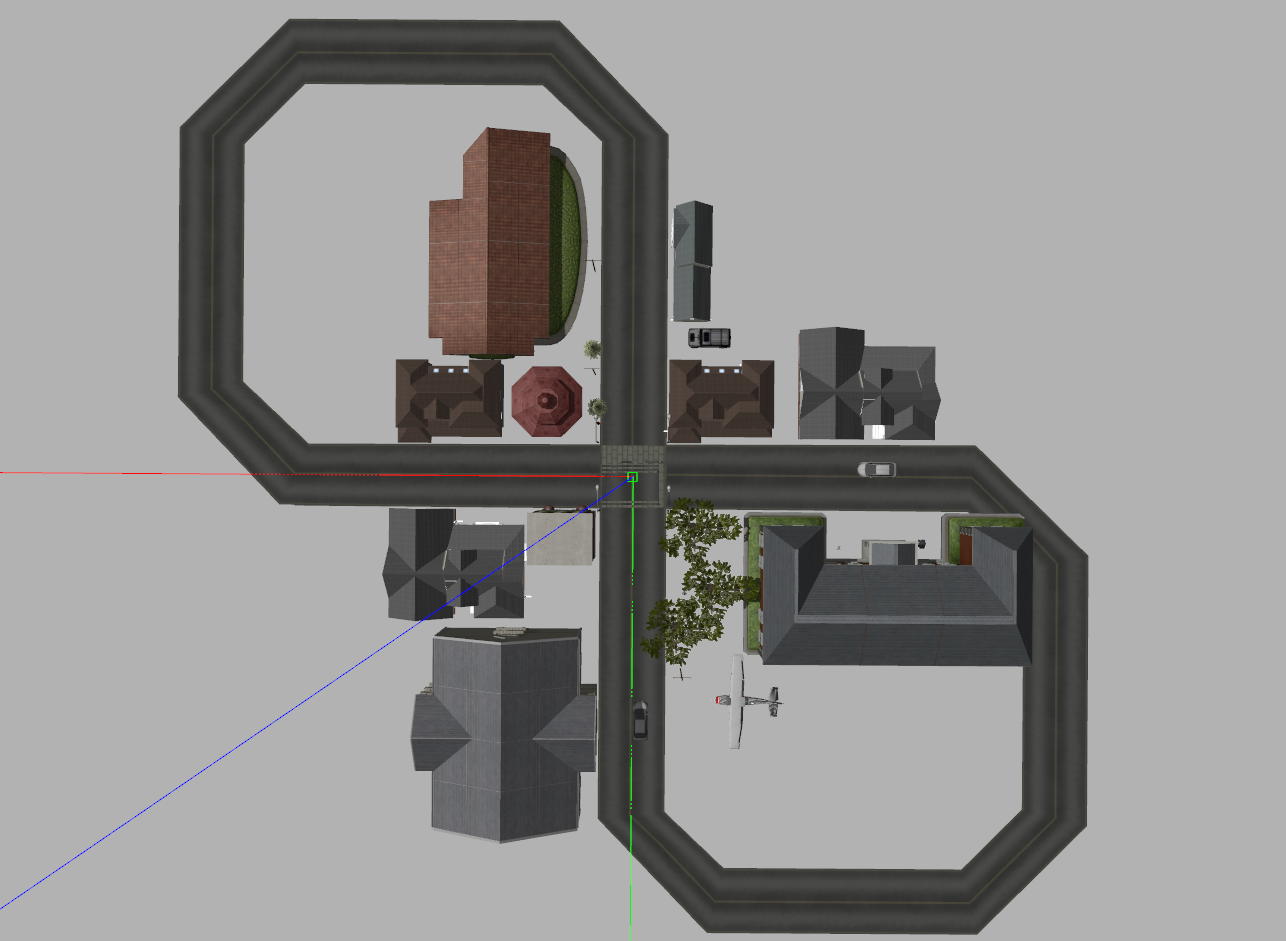
\includegraphics[width=0.7\paperwidth]{GazeboCrossroad.png}}
\end{center}
\caption{The simulated crossroad scenario in the Gazebo simulator.}
\label{fig:GazeboCrossroad} 
\end{figure}

The simulated vehicle in the virtual world are controlled using Gazebo ROS Controller which is a part of ROS packages names gzebo\_ros\_pkgs. This package provide the necessary modules and interfaces to simulate a robot (a vehicle in our case) in Gazebo which is taking orders from ROS messages and services. ROS is the short for "Robot Operating System" which is a robotics middleware that provide users with integrated packages, services and tools. The reusability for codes, implemented in multiple languages and continuous support from its community are all the benefits of ROS. 


The front, left and right views from the driver seat are directly projected onto the screens when driving in simulated world. (Fig.~\ref{fig:FrontCam}, Fig.~\ref{fig:LeftCam} and Fig.~\ref{fig:RightCam} respectively.) Control commands from the volunteers are sent from the joysticks to ROS node (a single process under ROS). Then the command velocity calculated according to the movement of the joystick is finally sent from the ROS node to the simulated vehicle in Gazebo. In every set of interaction experiments, a pair of volunteers (as shown in Fig.~\ref{fig:Driver1} and Fig.~\ref{fig:Driver2}) are asked to drive across the intersection without collision. The displacements to the node and the speed of vehicles for both driver are recorded with the time resolution of 0.01 sec. 

\begin{figure}[htbp!]
\begin{center}
\makebox[0pt]{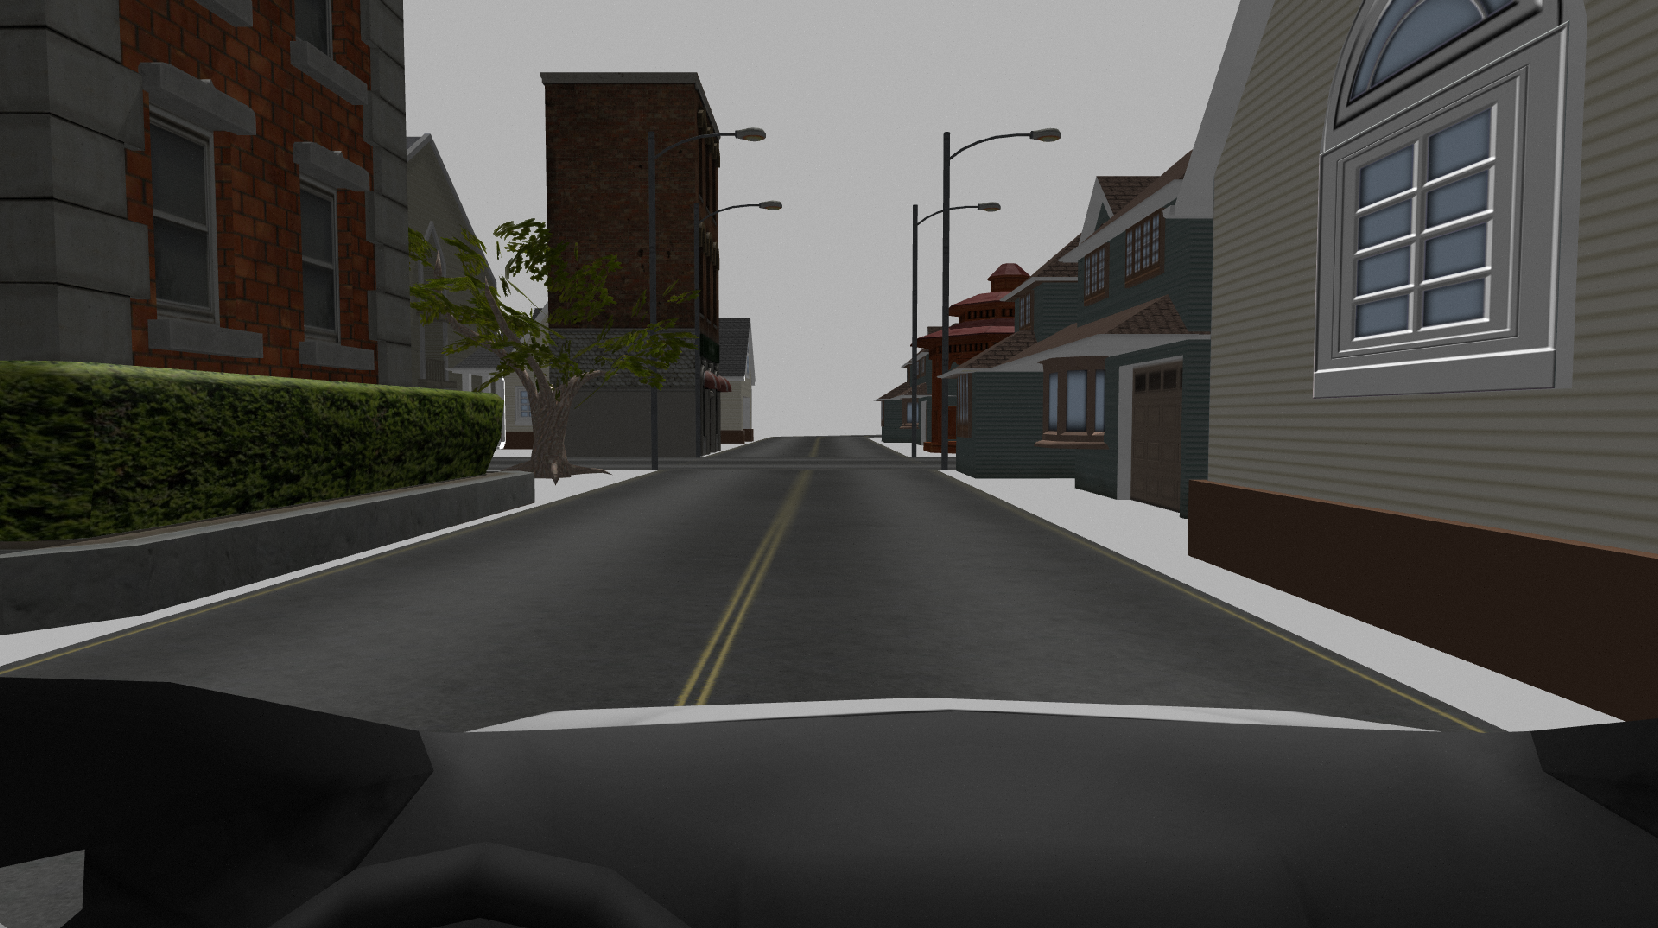
\includegraphics[width=0.7\paperwidth]{PriusFcam.png}}
\end{center}
\caption{Front camera from driver seat in the simulated environment.}
\label{fig:FrontCam} 
\end{figure}

\begin{figure}[htbp!]
\begin{center}
\makebox[0pt]{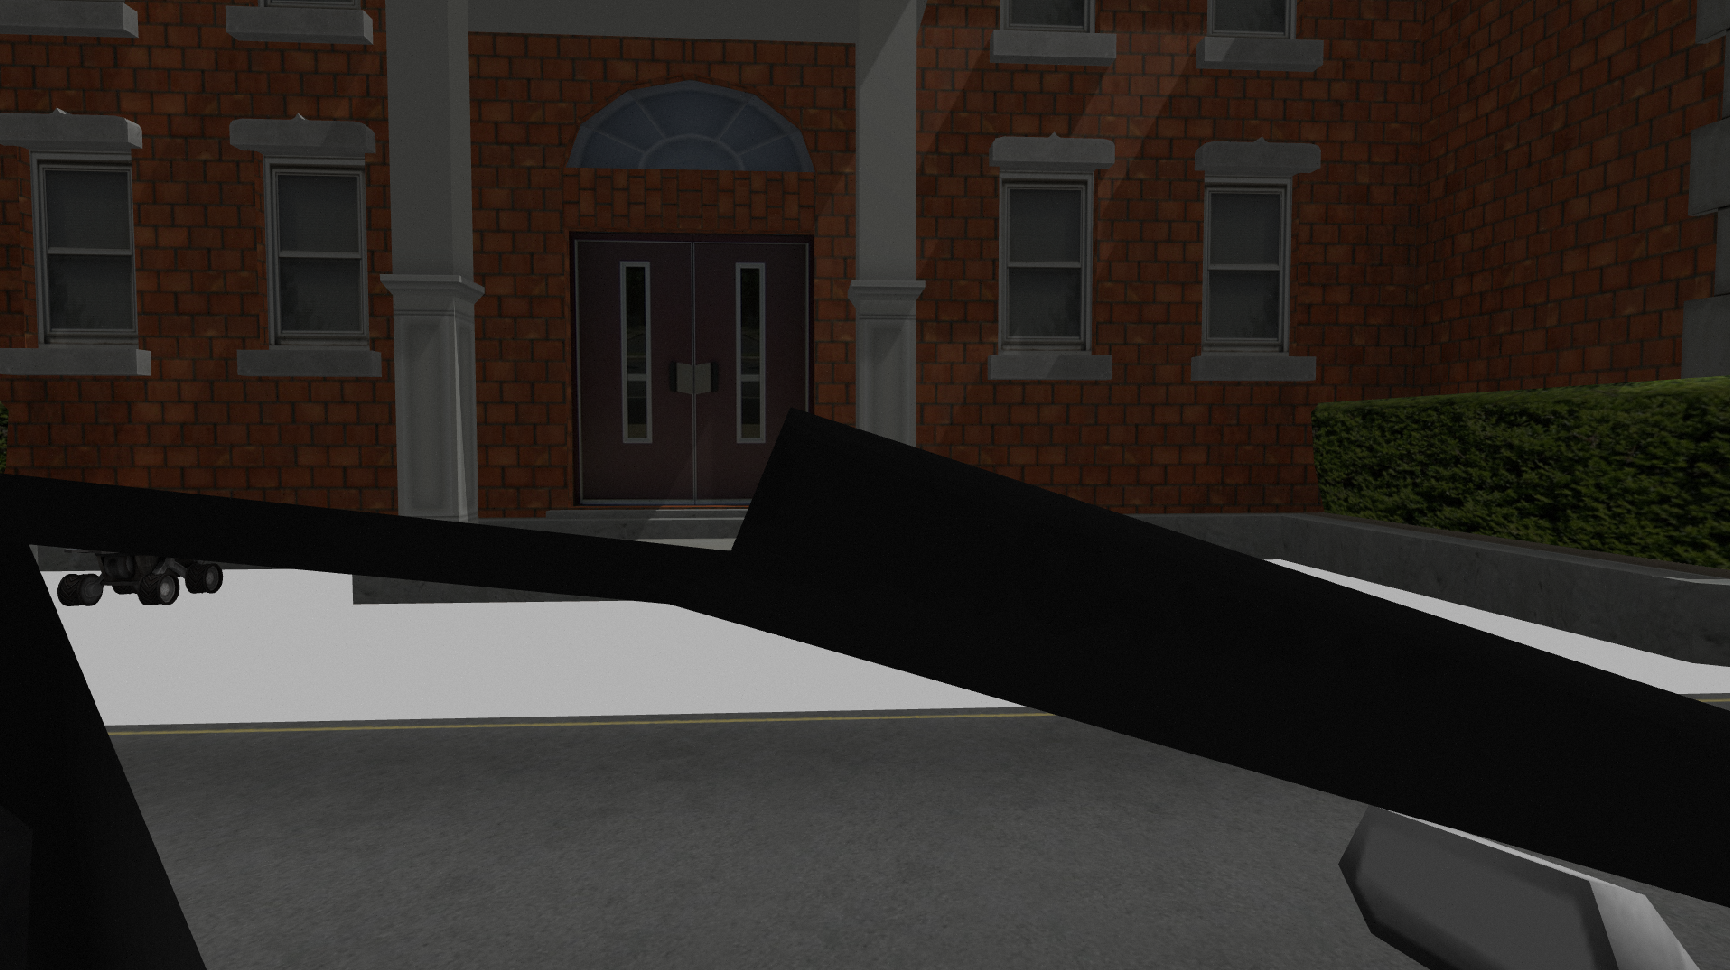
\includegraphics[width=0.7\paperwidth]{PriusLcam.png}}
\end{center}
\caption{Left camera from driver seat in the simulated environment.}
\label{fig:LeftCam} 
\end{figure}

\begin{figure}[htbp!]
\begin{center}
\makebox[0pt]{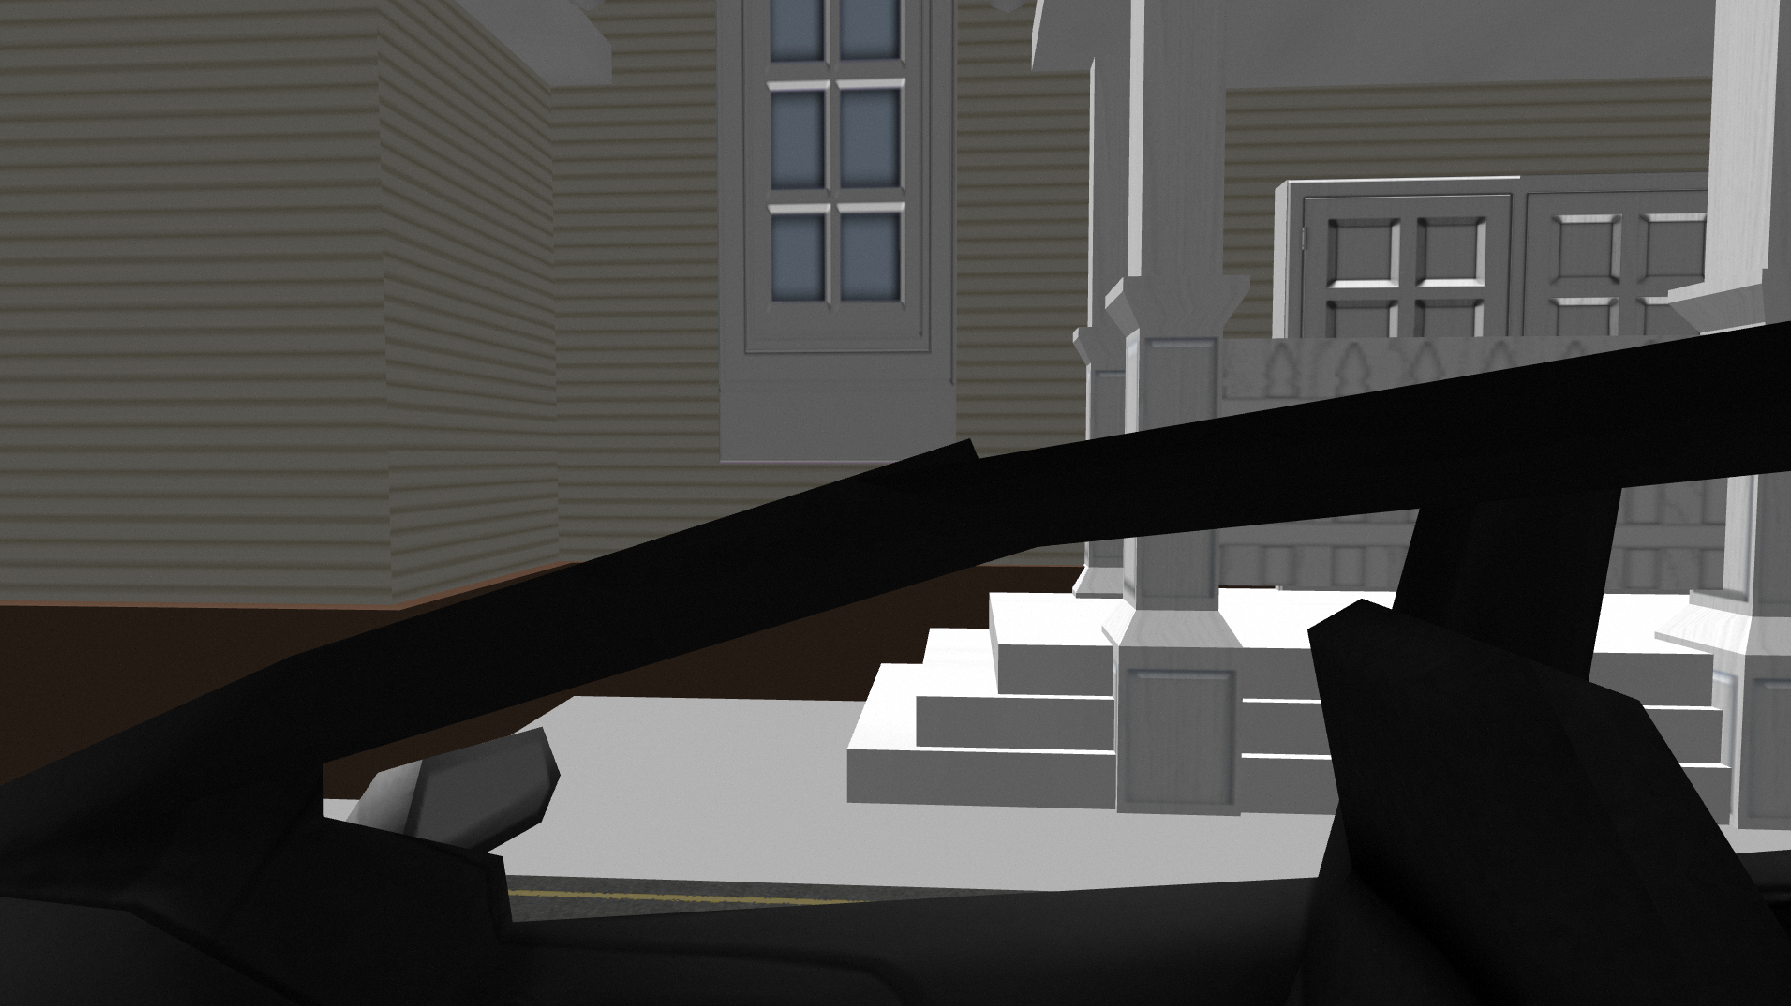
\includegraphics[width=0.7\paperwidth]{PriusRcam.png}}
\end{center}
\caption{Right camera from driver seat in the simulated environment.}
\label{fig:RightCam} 
\end{figure}

\begin{figure}[htbp!]
\begin{center}
\makebox[0pt]{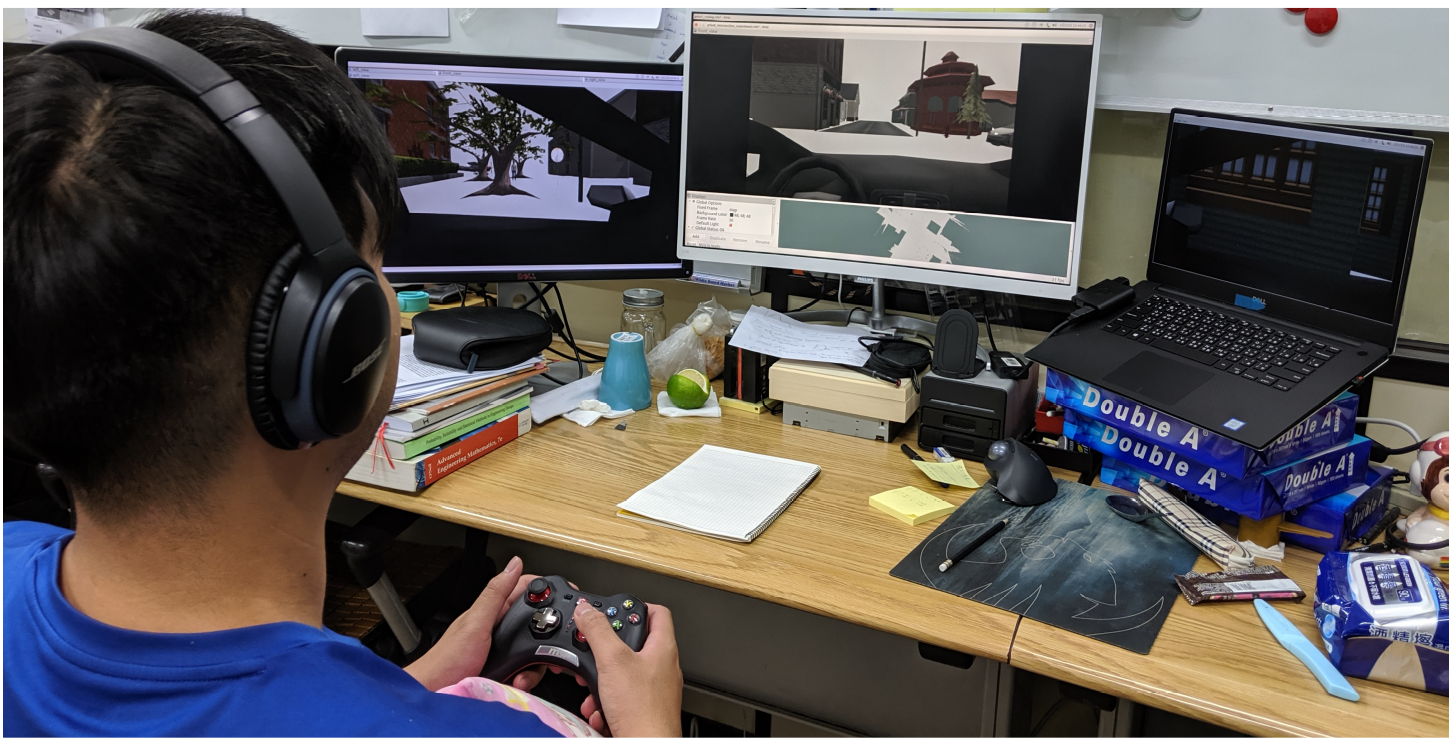
\includegraphics[width=0.7\paperwidth]{Driver1.png}}
\end{center}
\caption{First driver in the simulated crossroad interaction experiment.}
\label{fig:Driver1} 
\end{figure}

\begin{figure}[htbp!]
\begin{center}
\makebox[0pt]{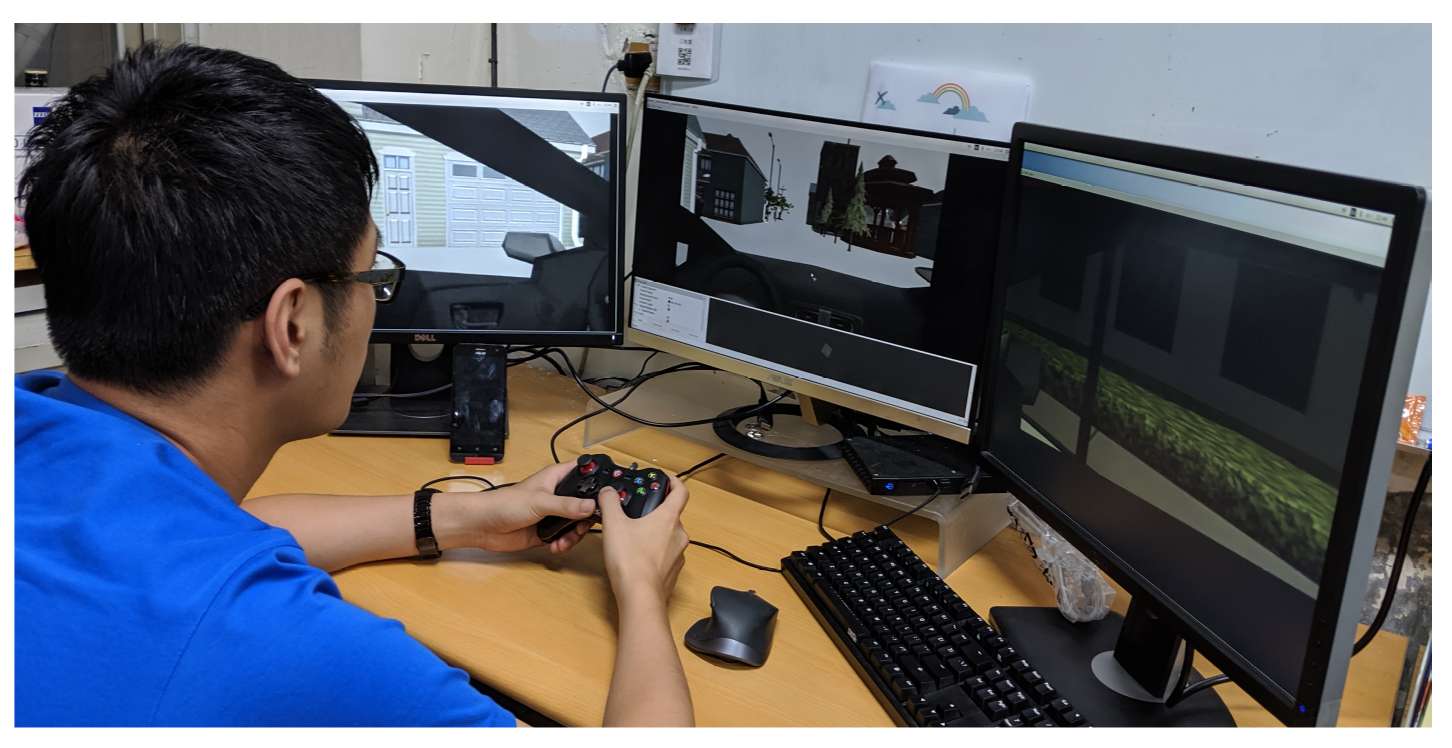
\includegraphics[width=0.7\paperwidth]{Driver2.png}}
\end{center}
\caption{Second driver in the simulated crossroad interaction experiment.}
\label{fig:Driver2} 
\end{figure}

%%%%%%%%------------------------------%%%%%%%%%
%%%%%%%%-----------SUBSECTION---------%%%%%%%%%
%%%%%%%%------------------------------%%%%%%%%%
\subsection{Experimental Results in Simulated Environment}
\label{sub:ResultSim}

Since there are three participants who are asked to participate in pair, and about 50 repetitions were conducted each pair, so there will be about 150 sets of data in total. Within these trials, some will be explained in detail to demonstrate the performance of the proposed model. Then the classification accuracy rate will be evaluated using all data sets for validation.  

\begin{figure}[htbp!]
    \centering
    \subfloat[Illustration of calculated TTC of each vehicle.]
    {
    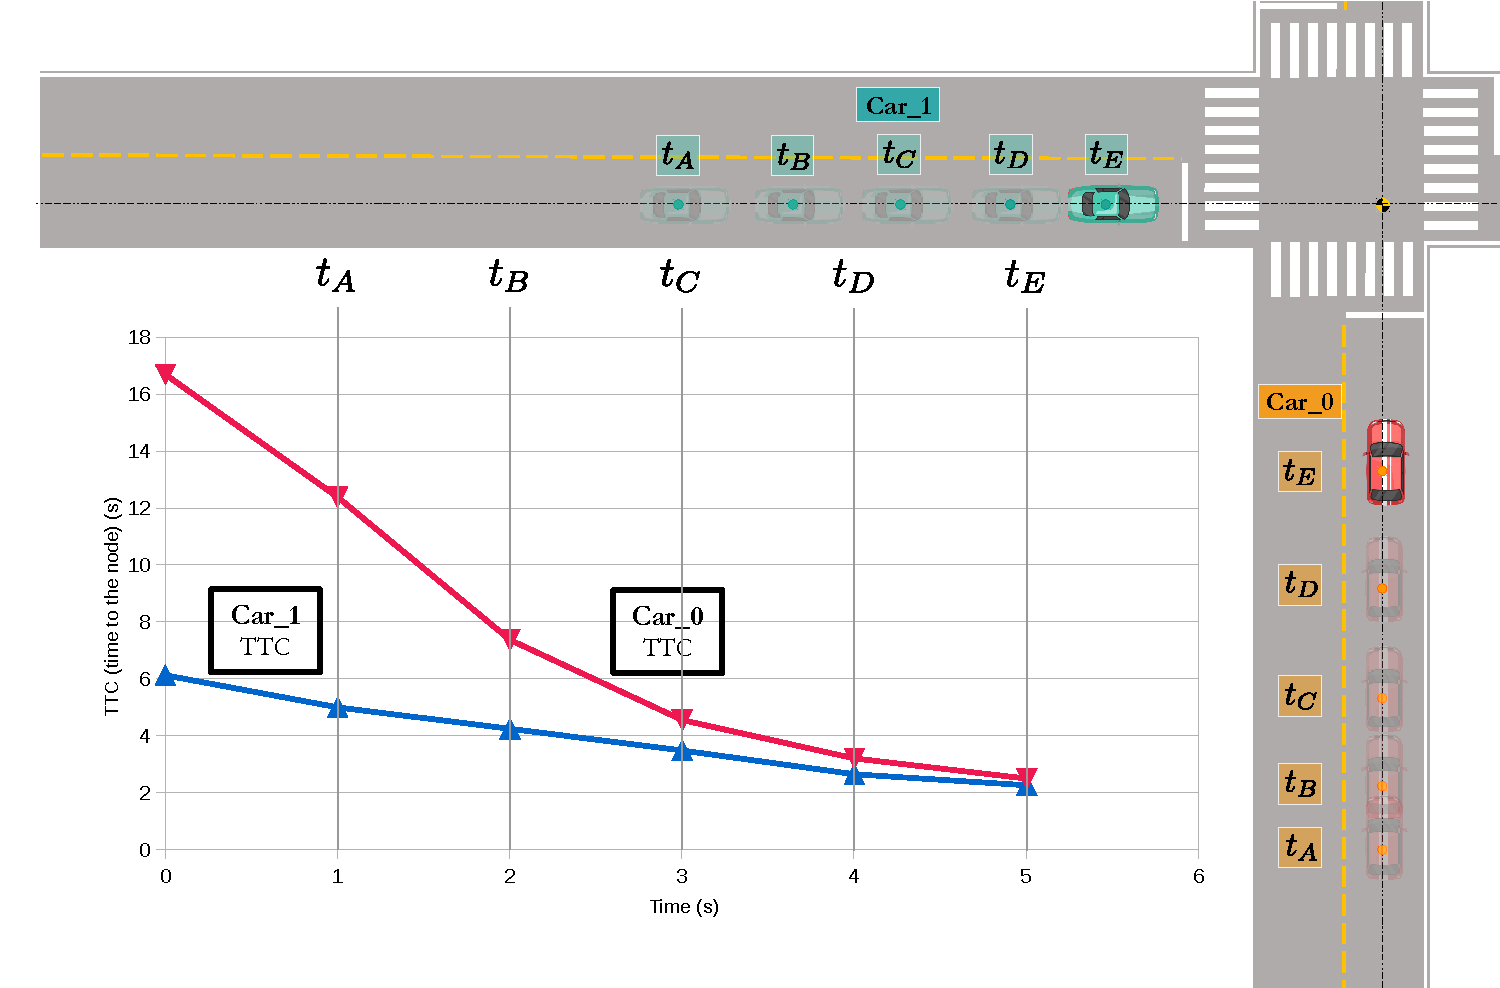
\includegraphics[width=0.47\textwidth]{figure_explaination_TTC.pdf}
    \label{fig:figure_explaination_TTC}
    }\hfill
    \subfloat[Illustration of probability of stopping together with velocity and displacement.]
    {
    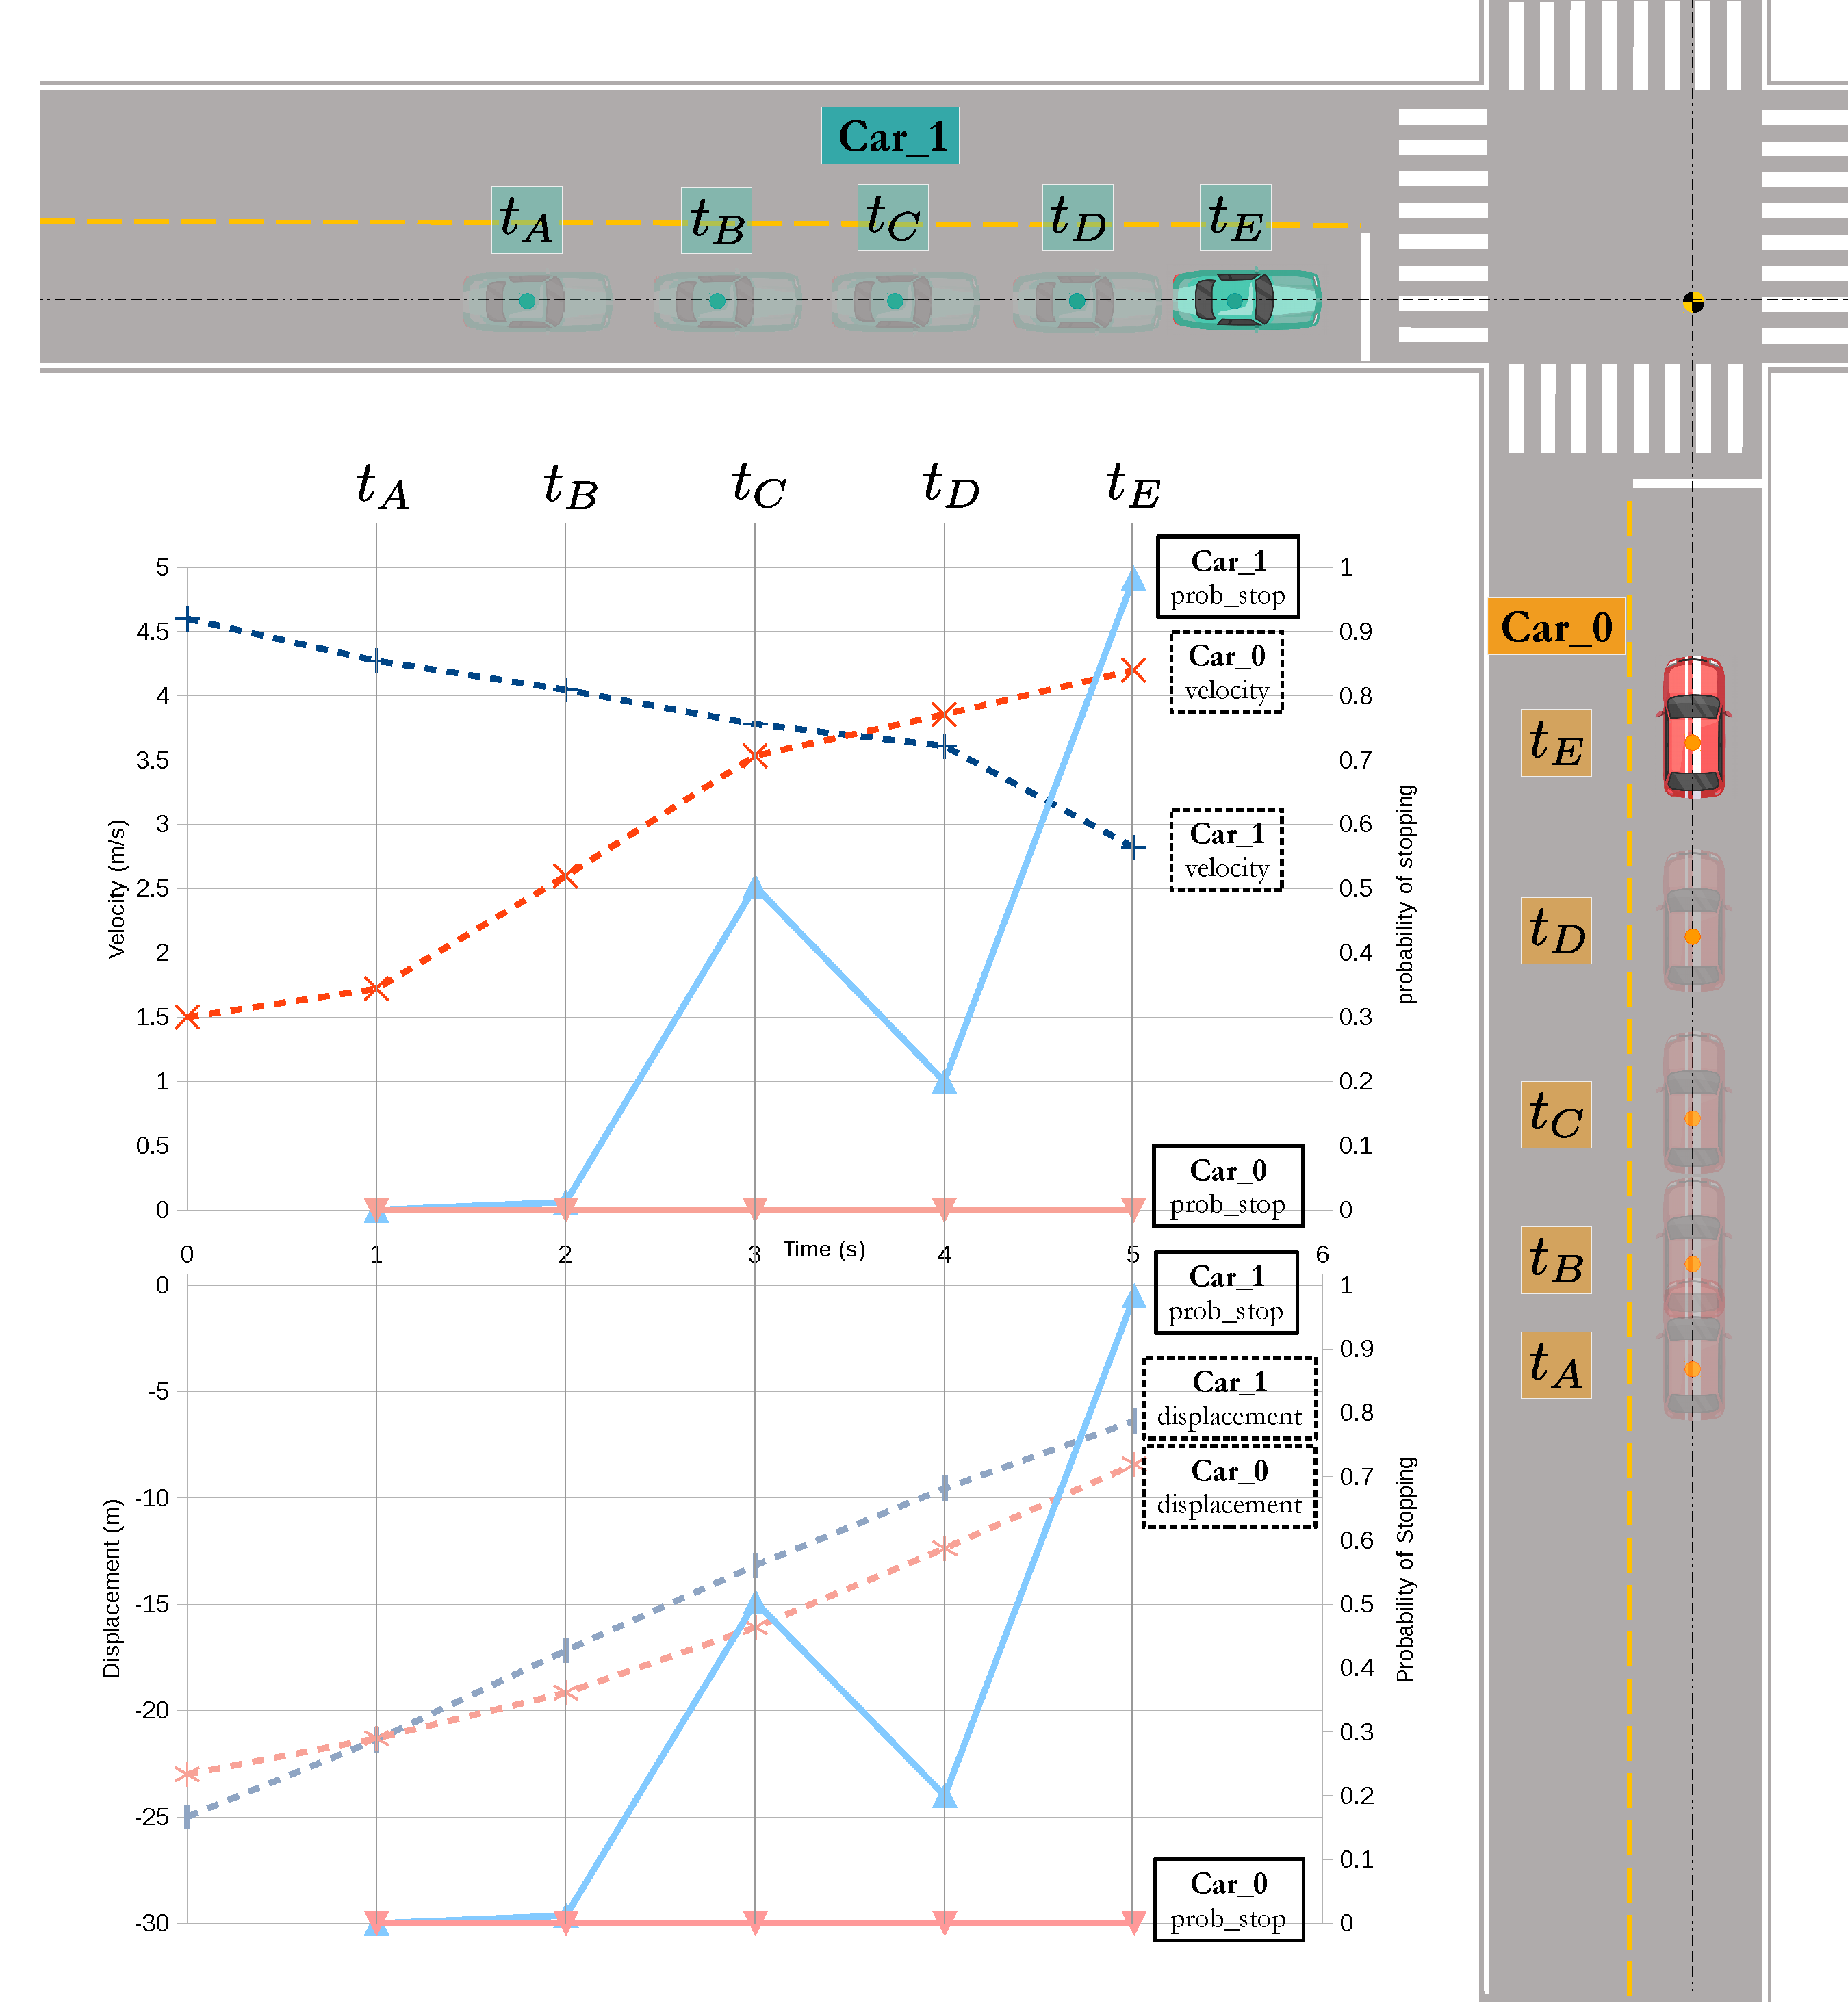
\includegraphics[width=0.47\textwidth]{figure_explaination_1.pdf}
    \label{fig:figure_explaination_1}
    }\hfill
    
    \caption{Illustration of TTC and probability of stopping along with concerning variables.} \label{fig:illustration}
\end{figure}

We start the analysis by calculating the corresponding TTC of Car\_0 (in red) and Car\_1 (in cyan), as illustrated in Fig.~\ref{fig:figure_explaination_TTC}. TTCs correspond to $t_A$, $t_B$, $t_C$, $t_D$ and $t_E$ are shown in the chart of the figure. Afterward, the probability of stopping for each car is calculated using the proposed method and is plotted together with the velocity and the displacement in two separate figures, as illustrated in Fig.~\ref{fig:figure_explaination_1}. The data collection begins when both of the displacements to the node is smaller than 18 meters where drivers are able to see each other, and ends when the node is reached by one of the participants. We then analyze how the probability of stopping can give assistance to the traffic participants using these figures.


Next, some of the experiments results will be presented to evaluate the performance of the proposed model. There will also be further explanations about the importance of parameters in the model. In the experiment conducted, trials are labeled with number (e.g. \#001, \#002, ...). The first interaction observed is trial \#003. 

\begin{figure}[htbp!]
\begin{center}
\makebox[0pt]{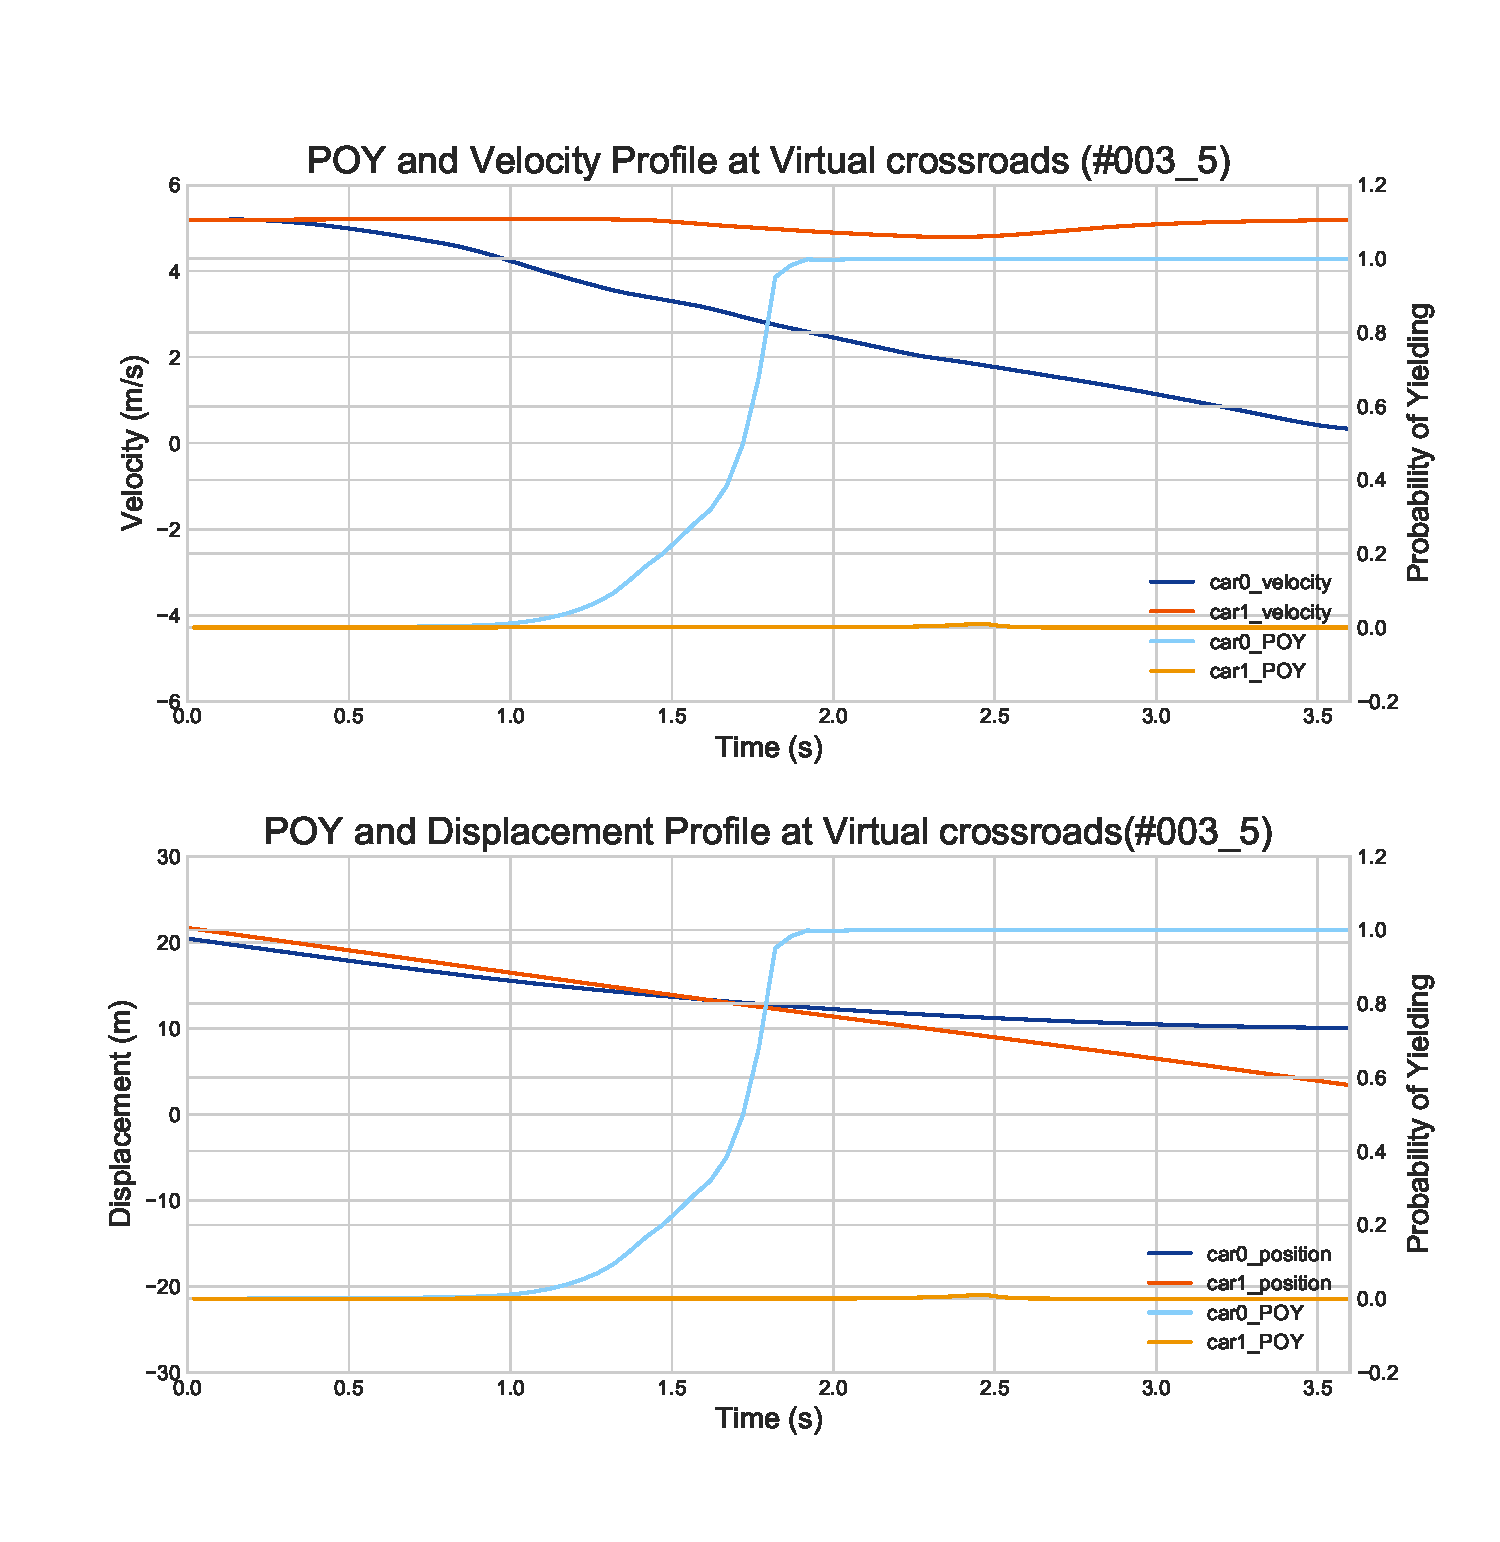
\includegraphics[width=0.65\paperwidth]{trial_003.pdf}}
\end{center}
\caption{Trial \#003 where car\_0 was yielding and car\_1 was passing with little interaction.}
\label{fig:trial003} 
\end{figure}

In this case, both yielding and passing types of drivers were included in this scene. Yielding type of drivers are those who will stop relatively early before the node, and slowly approach the intersection. They would only pass when the other agent is yielding. The passing type is the opposite, where there will be almost zero braking applied during the whole process. 


As presented in Fig.~\ref{fig:trial003}, driver of car\_0 was the yielding type because the deceleration started as soon as they could see each other in the sight (displacement at around 15 to 18 meters), and the driver of car\_1 was the passing type. During 0.8 to 1.8 sec, the POY of car\_0 was rising mainly due to the decreasing of the TTC at the moment, which was becoming smaller than the $TTA_{est}$ and resulted in more and more areas were under the TFA distribution and right to the TTC. The small spike on the POY curve of car\_1 around 2.5 was owing to the braking applied at about the same moment. In the next but one figure, this little bump will be elaborated. In this figure, the outcome suggests that the proposed model can correctly estimate the intention of the driver on other moving vehicles about 2 secs earlier.


\newpage


\begin{figure}[htbp!]
\begin{center}
\makebox[0pt]{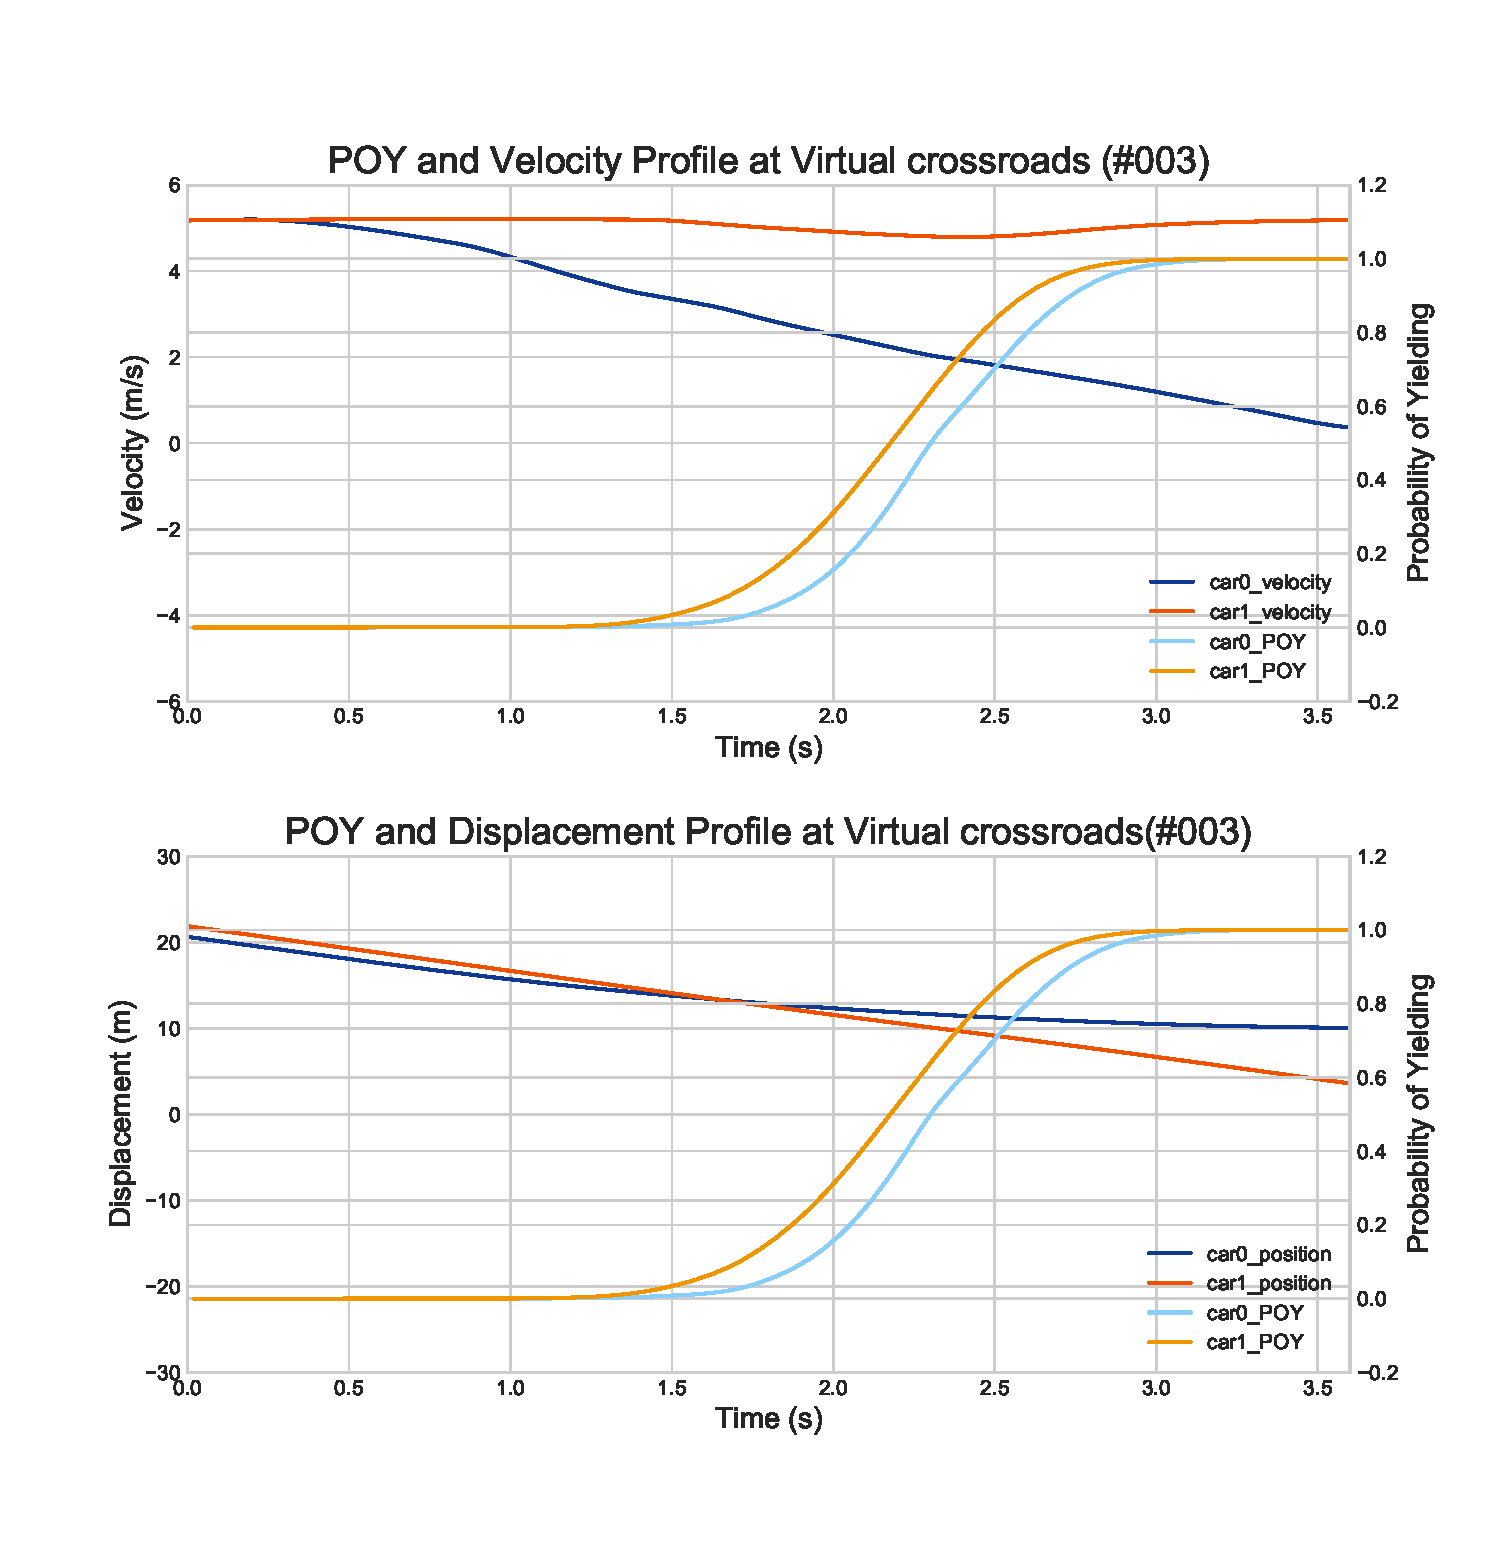
\includegraphics[width=0.65\paperwidth]{trial_003_WOalpha.pdf}}
\end{center}
\caption{Trial \#003 using POY without weighting parameter $A$ ($\alpha$).}
\label{fig:trial003WOalpha} 
\end{figure}



To demonstrate the importance of the weighting parameter $A$ ($\alpha$), which was formulated in Chapter \ref{chap:DriverModel}, the same trial (trial \#003) was evaluated again using the proposed POY model, but without the parameter $A$ ($\alpha$). Results are shown in Fig.~\ref{fig:trial003WOalpha}. Note that the POY of both vehicles rose to 1.0 from 1 to 3 sec. The main factor in this scenario was the displacement to the node which affected the $TFA_{est}$ and the $min TTC$. The plot showed that the closer the vehicle to the node, the higher the POY will be if it only depends on the displacement. Without the parameter $A$ ($\alpha$) being able to account for the acceleration and velocity and provide adjustments accordingly, the POY is unable to predict accurately. 

The conditions in Eqn.~\ref{eq:alpha} were also proved to be indispensable for the proposed model to produce a stable result in Fig.~\ref{fig:trial003WOcondition}. The huge spike occurred on the curve of car\_1 POY around 1.2 to 2.5 secs was the consequence of the proposed model being too "sensitive" about some small changes in acceleration that usually do not imply the intention to yield. Constraints such as the maximum deviation for the TFA distribution (as formulated in Eqn.~\ref{eq:alpha_cap}) or the threshold for acceleration longer than 0.2 sec are employed to prevent the POY from being too sensitive to accelerations.

\begin{figure}[htbp!]
\begin{center}
\makebox[0pt]{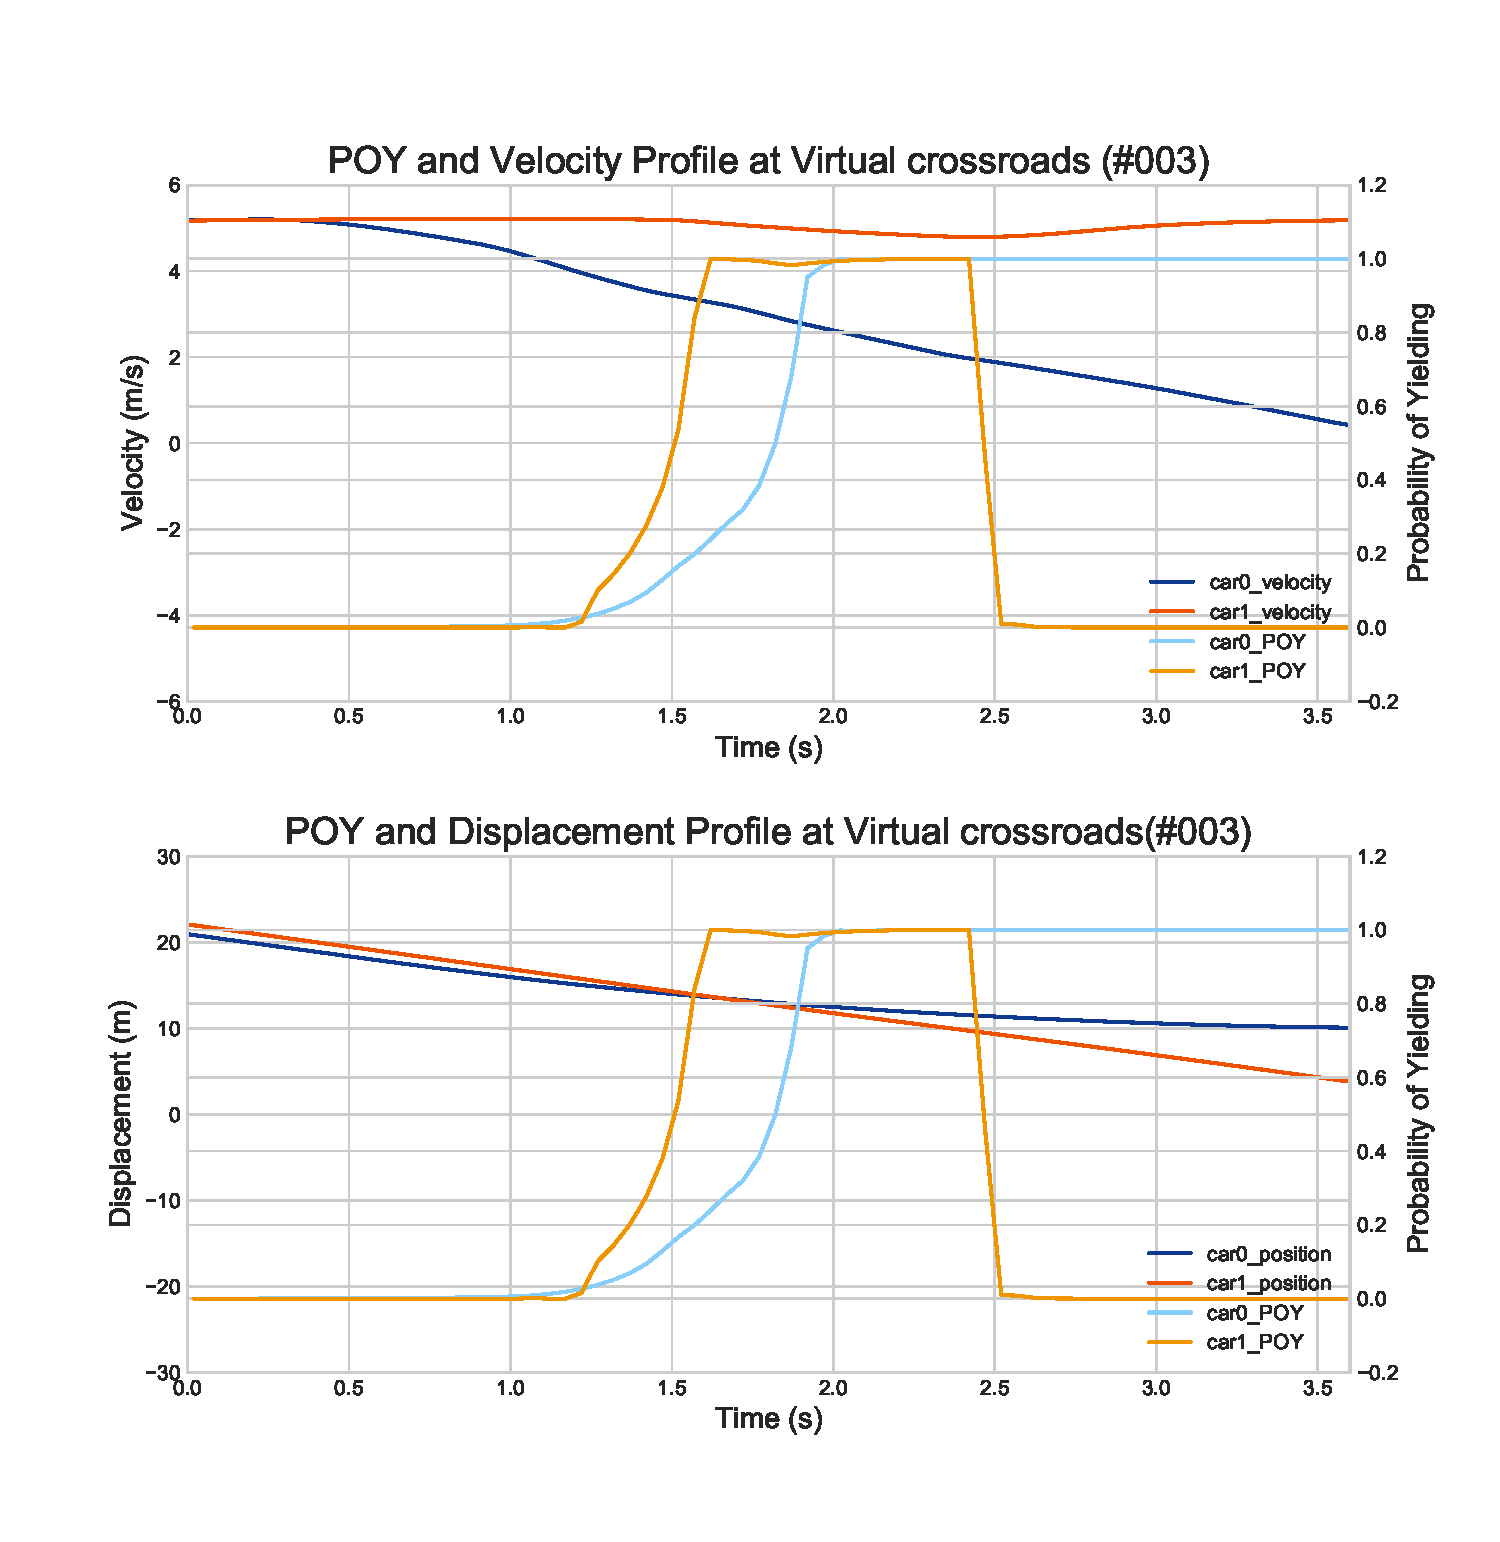
\includegraphics[width=0.65\paperwidth]{trial_003_WOcondition.pdf}}
\end{center}
\caption{Trial \#003 using POY without acceleration threshold.}
\label{fig:trial003WOcondition} 
\end{figure}


The second case of interaction is more interactive than trial \#003. In trial \#077, both drivers were indecisive, since both participants were quite even at their states and no one was in dominant position. In the most extreme cases, it will take both drivers quite a long time before one of them decides to pass or yield. In trial \#077, however, it did not take them too long before car\_0 finally decide to pass. At the beginning of the interaction, POYs of both vehicles rose due to their deceleration. And from 1.5 to 3.2 secs, the POYs were kept at high level for car\_0, while car\_1 had the intention to pass, which resulted in the drop of POY. But right after car\_1 accelerated, so did car\_0 with very small time difference (0.5 sec). And after about a second, they both decelerated together again, but this time car\_1 was determined to yield and car\_0 finally passed. During this time, human drivers had no information about what actions the other one intended to take, so they waited until one of them did something. Yet, if one could utilize the proposed model which could estimate the TFA distribution of the driver and generate a probability from his or her current states, this stnad-off-like situation could have been avoided. 

\begin{figure}[htbp!]
\begin{center}
\makebox[0pt]{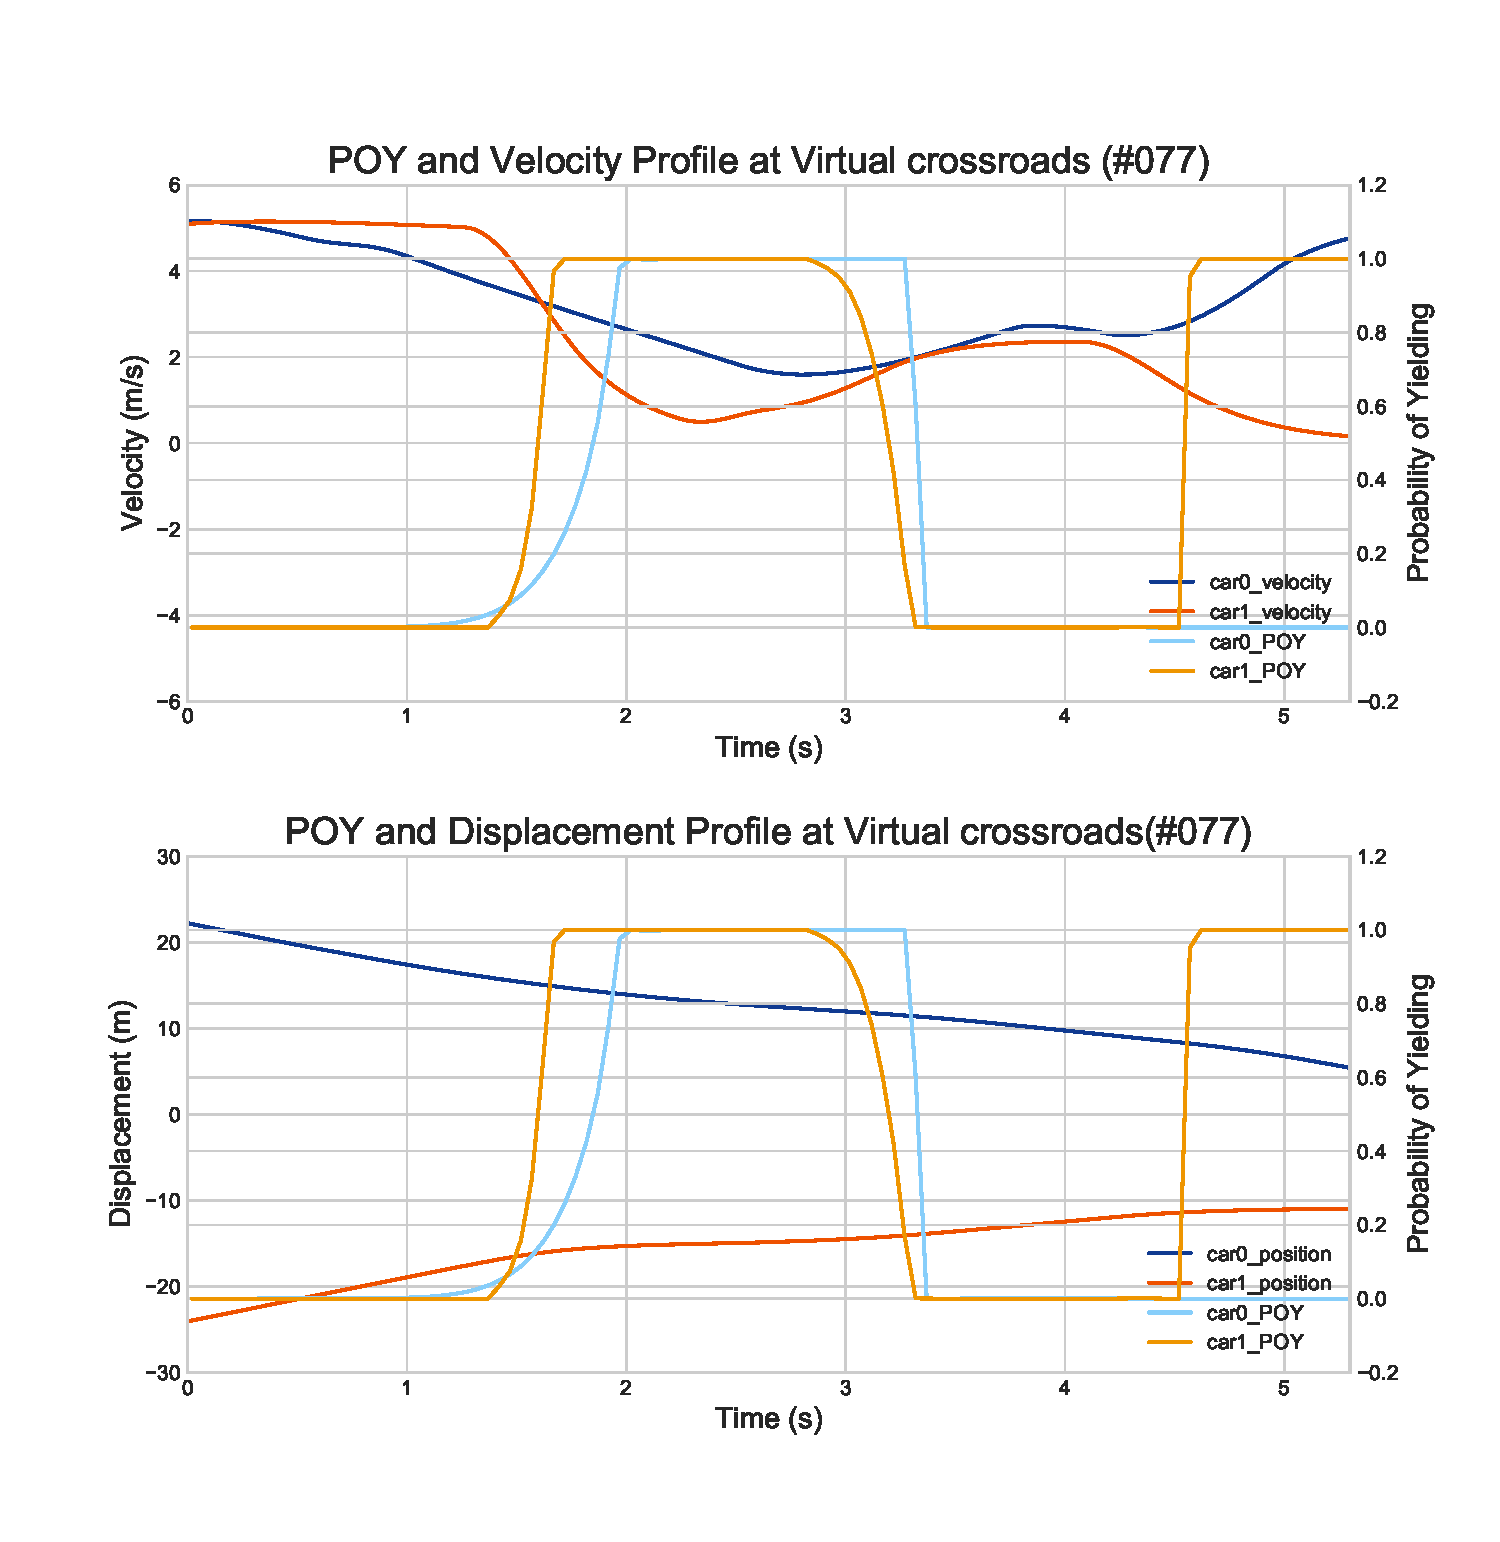
\includegraphics[width=0.65\paperwidth]{trial_077_indecisive.pdf}}
\end{center}
\caption{Trial \#077 where car\_0 and car\_1 were confused about what action the other one might take.}
\label{fig:trial077} 
\end{figure}


The final case presented can again show how one can benefit from the proposed model. In Fig.~\ref{fig:trial063}, car\_0 was a bit closer to the node and it yielded to let car\_1, who was farther but had no intention to yield, passed first. However, car\_1 did not think that the deceleration of car\_0 was intended to yield, so it chose to yield too and car\_0 then accelerated to pass. Again, this situation could have been avoided if the proposed method is referenced by the driver.


\begin{figure}[htbp!]
\begin{center}
\makebox[0pt]{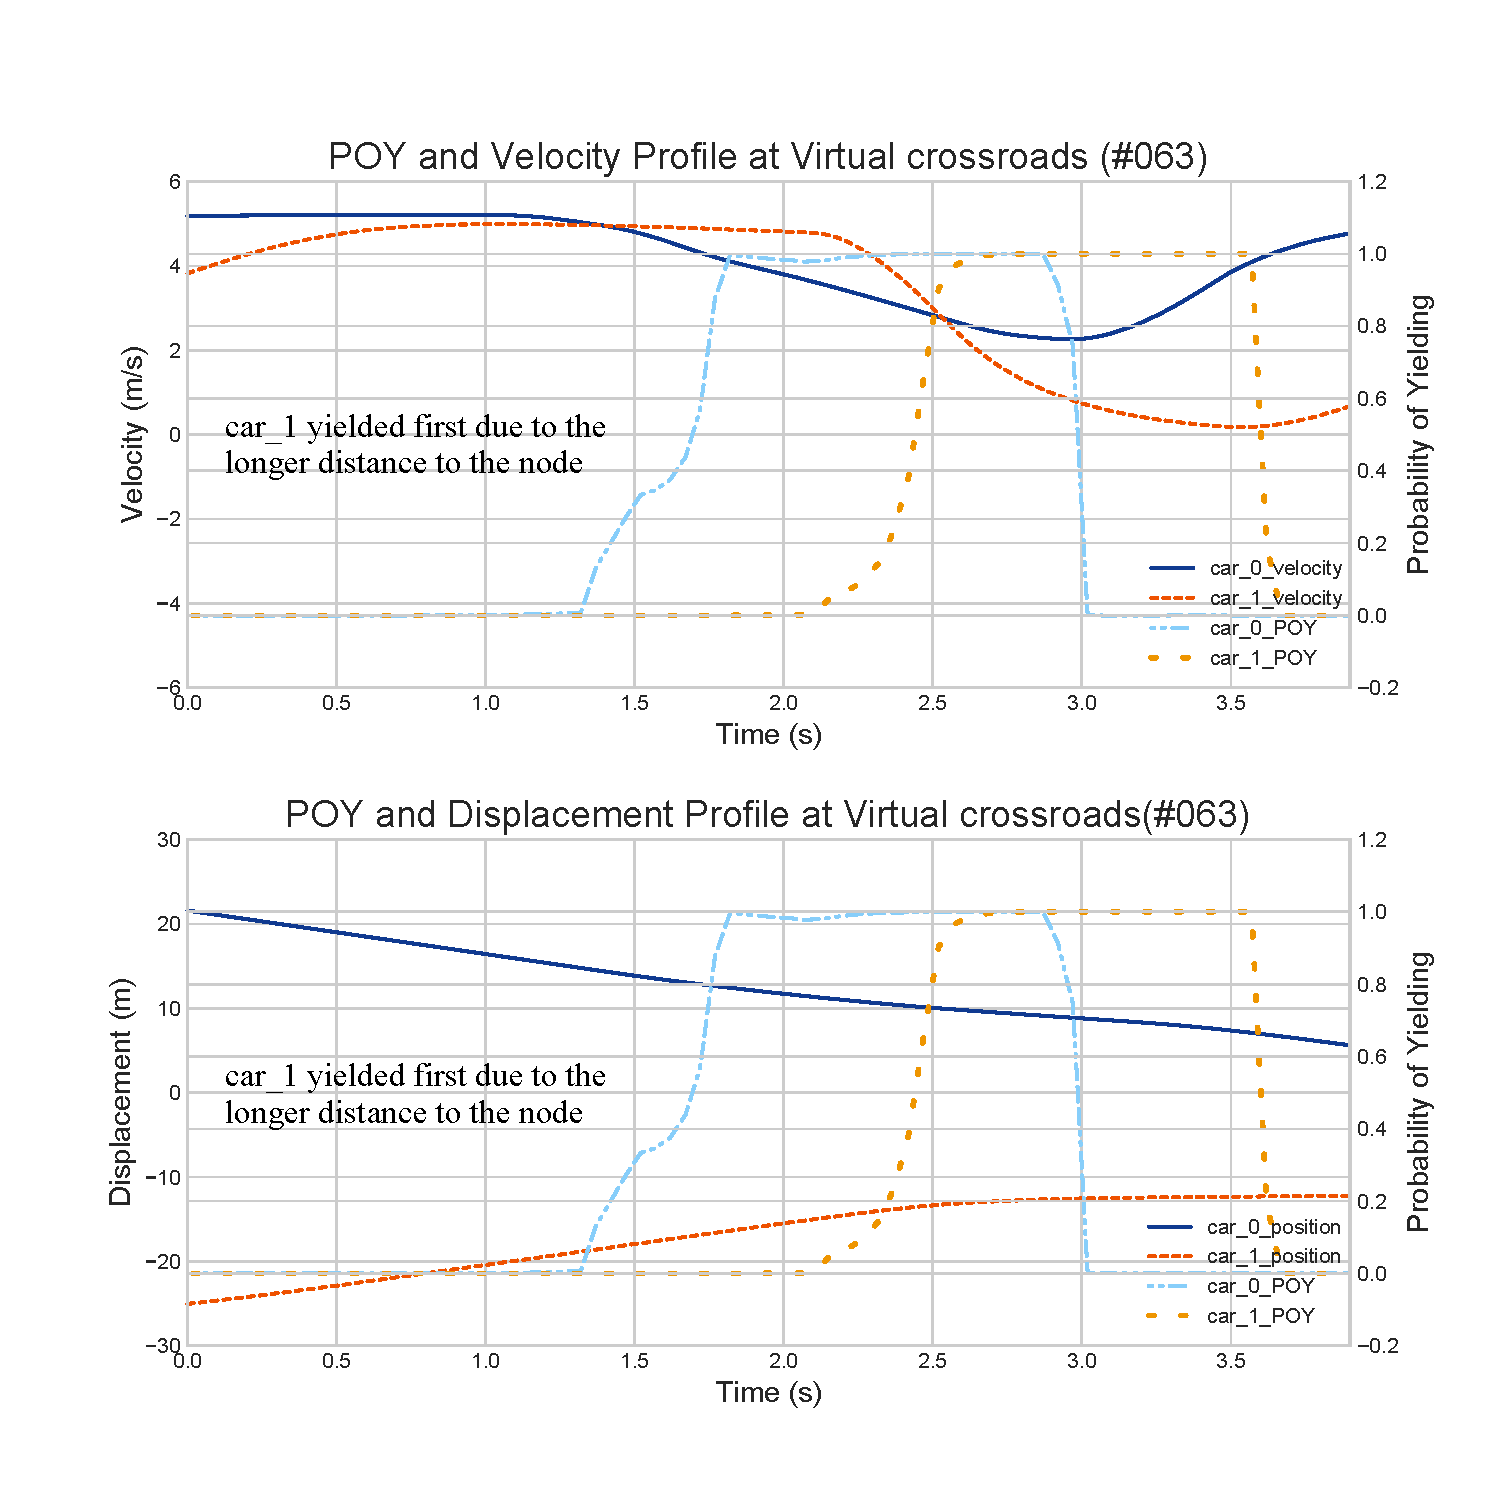
\includegraphics[width=0.65\paperwidth]{trial_063_bothyield.pdf}}
\end{center}
\caption{Trial \#063 where car\_0 yielded first but then passed due to the deceleration of car\_1 .}
\label{fig:trial063} 
\end{figure}

\newpage

%%%%%%%%------------------------------%%%%%%%%%
%%%%%%%%-----------SUBSECTION---------%%%%%%%%%
%%%%%%%%------------------------------%%%%%%%%%
\subsection{Validation for Experiments in Simulated Environment}
\label{sub:ValidationSim}


In Section \ref{sub:ResultSim}, the proposed model is proved to be comparable to human drivers' prediction and the decisions of human drivers are managed to turn into some probabilistic values, which can be perceived by autonomous vehicles. In this section, the accuracy of the proposed model will be examined.

\begin{equation}
    CARate = \frac{\text{number of correctly classified situations}}{\text{number of all situations}}
\label{eq:CARate}
\end{equation}

The \ac{CARate} is used to evaluate the calssification accuracy of the proposed model. Due to the fact that the time spans for all interaction trials are different, the time line is be reversed and denoted as $T_{minus}$, i.e., $T_{minus}=0$ denotes the time at the end of the process and $T_{minus}=1$ denotes the time 1 sec earlier than that, and so on. Note that the end of the process is defined as the moment which the node is reached by one of the participants. The calculation of CARate is rather straight forward as shown in Eqn.~\ref{eq:CARate}. In the total of 168 cases of driver behaviors at the crossroad, the denominator of the CARate at each $T_{minus}$ is then 168. The CARate results of the proposed model are shown in Fig.~\ref{fig:CARPOY}.

\begin{figure}[htbp!]
\begin{center}
\makebox[0pt]{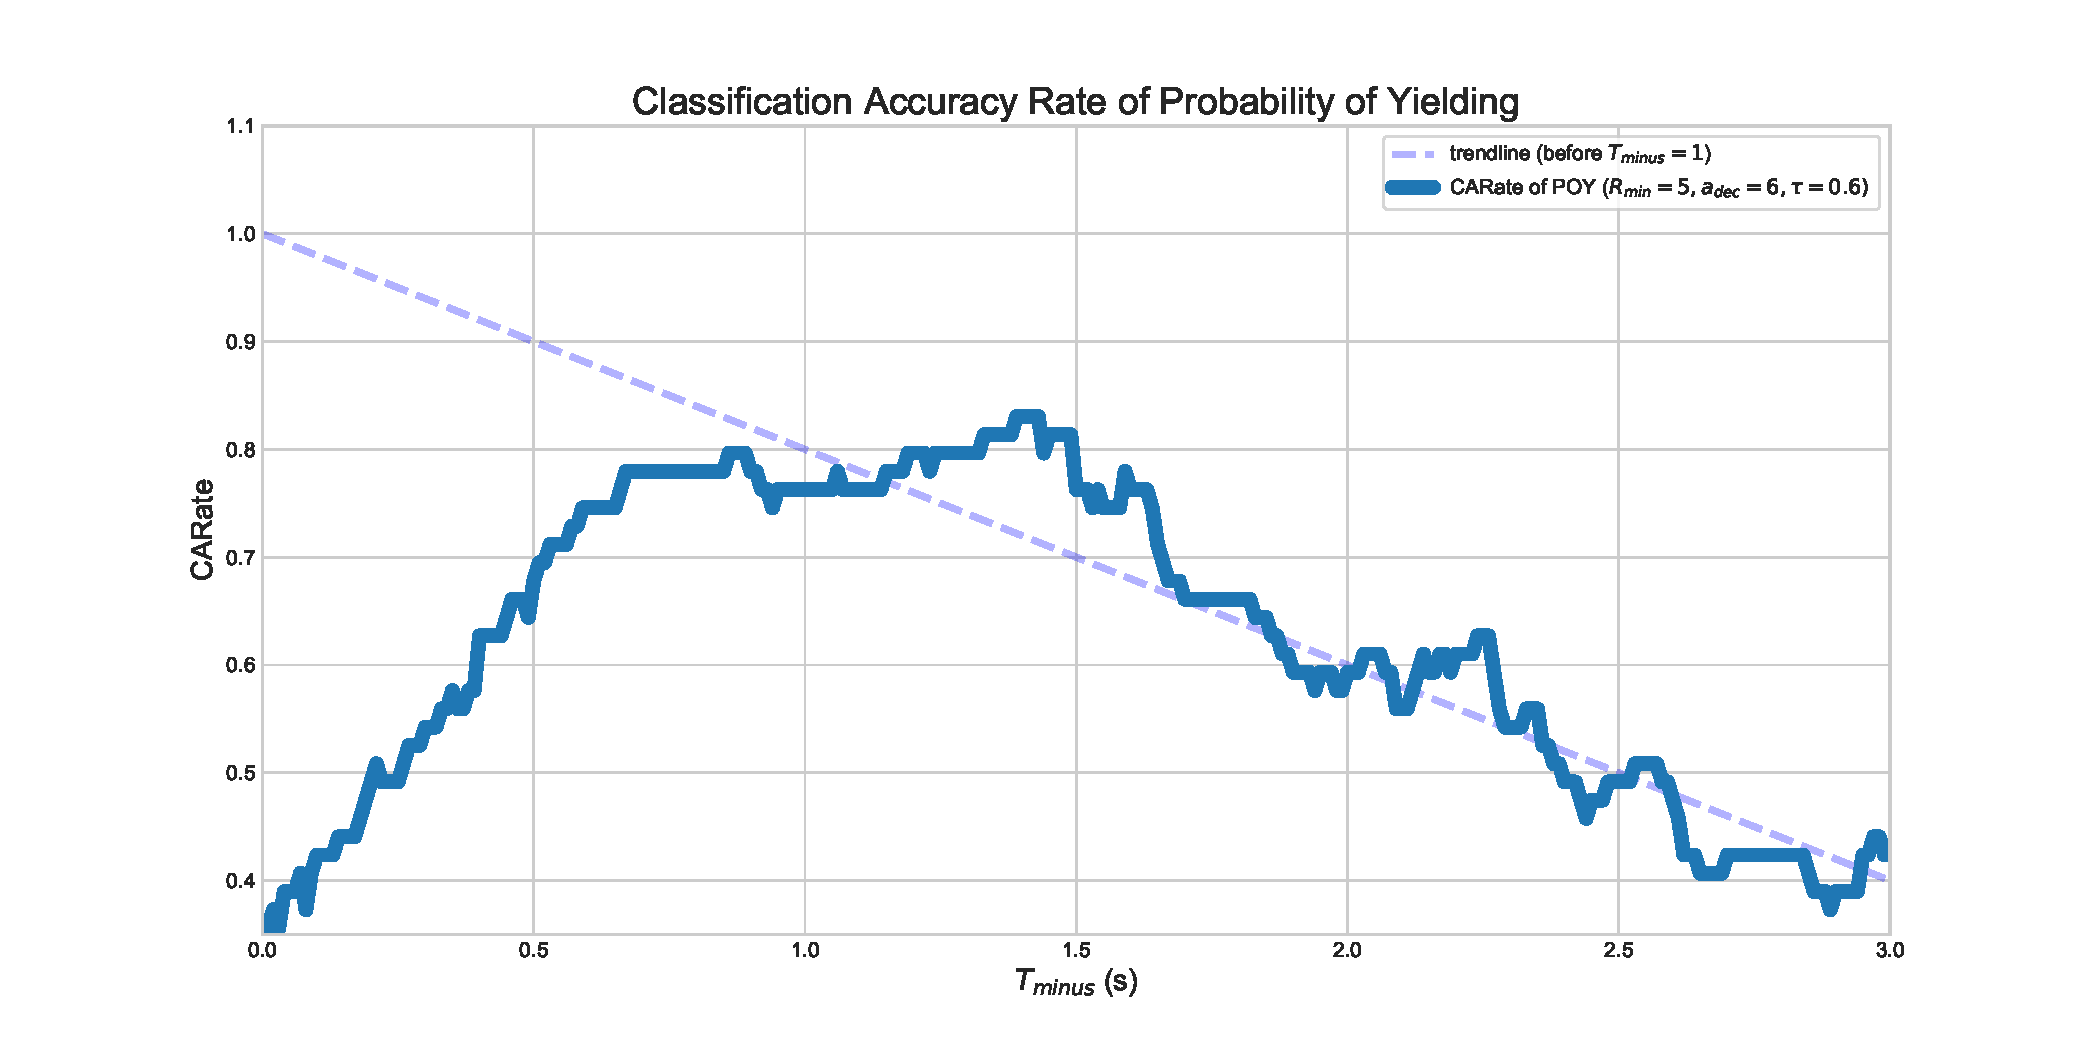
\includegraphics[width=0.72\paperwidth]{CARPOY.pdf}}
\end{center}
\caption{CARate of the POY using all data sets.}
\label{fig:CARPOY} 
\end{figure}

Results using the average parameters listed in Table.~\ref{table:parameters} are plotted in solid blue line while the trend line is plotted in dashed blue line. The reason for the drop from 0.0 to 1.5 $T_{minus}$ is that, people tend to behave more aggressive in our simulated environments. During the experiment, participants who yielded for the other driver accelerated before the end of the process which is the moment when the node is reached. The example is shown in Fig.~\ref{fig:trial039}.

\begin{figure}[htbp!]
\begin{center}
\makebox[0pt]{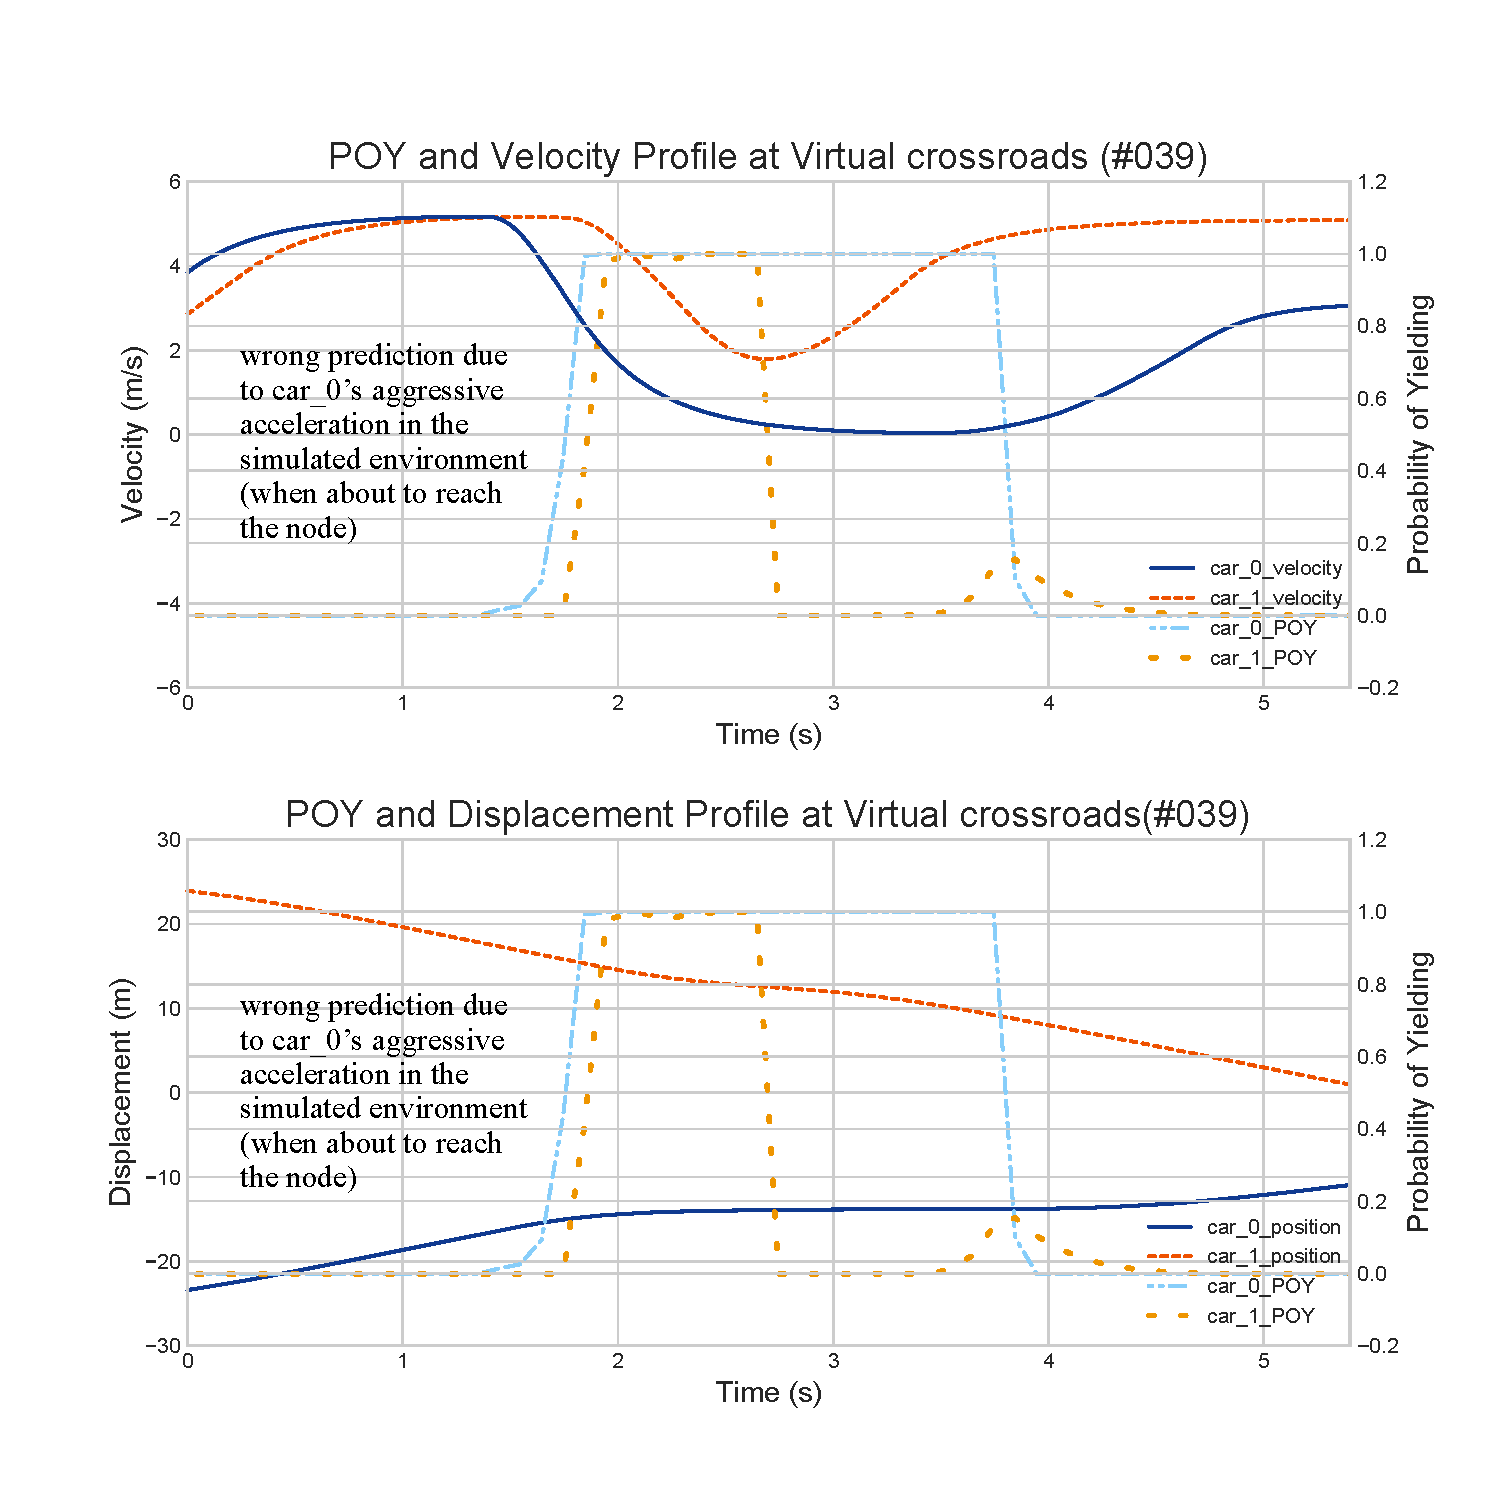
\includegraphics[width=0.65\paperwidth]{trial_039_toosoon.pdf}}
\end{center}
\caption{Trial \#039 where car\_1 begun to accelerate before car\_0 passed the node, causing the false prediction.}
\label{fig:trial039} 
\end{figure}

Comparing to other few behavior prediction model, the CARate of the proposed model is comparable to the state-of-the-art. In the work of Graf et al. \cite{Graf2014}, the CARate reached 0.81 at around $T_{minus} = 3$, while in the proposed model 0.81 is reached at $T_{minus} = 1.5$. This is owing to the relatively short interaction time span in the simulated environment, where participants are using joysticks sending out maximum command velocity. In the literature, interactions at real crossroads takes about 6 secs to cross a 12 to 18 meters long distance, yet at the simulated crossroad, it only takes about 3.5 secs to cross 20 meters. Furthermore, the method proposed in the literature requires pre-trained model for a specific where in POY no training steps are needed. The proposed POY also has the potential of generating better predictions if the parameters characterizing his or her driving pattern is known.


In this chapter, a novel driver behaviors model at crossroads was proposed. Driver intentions were predicted based on the parameter TTC, which is an important and well developed risk estimation method in traffic safety assessment. Derived form the concept, the TFA distribution was shown to be an innovative and effective driver intentions indicator that can be used to predict the driver behaviors. The normally distributed TFA distribution was then formulated and proven to be an unerring approximation. At last the driver behaviors model was finally proposed and validated at the simulated crossroad where prediction accuracy was comparable to the state-of-the-art driver behaviors prediction method. 